
\documentclass[10pt]{article} % For LaTeX2e
\usepackage{tmlr}
% If accepted, instead use the following line for the camera-ready submission:
%\usepackage[accepted]{tmlr}
% To de-anonymize and remove mentions to TMLR (for example for posting to preprint servers), instead use the following:
%\usepackage[preprint]{tmlr}

% Optional math commands from https://github.com/goodfeli/dlbook_notation.
%%%%% NEW MATH DEFINITIONS %%%%%

\usepackage{amsmath,amsfonts,bm}

% Mark sections of captions for referring to divisions of figures
\newcommand{\figleft}{{\em (Left)}}
\newcommand{\figcenter}{{\em (Center)}}
\newcommand{\figright}{{\em (Right)}}
\newcommand{\figtop}{{\em (Top)}}
\newcommand{\figbottom}{{\em (Bottom)}}
\newcommand{\captiona}{{\em (a)}}
\newcommand{\captionb}{{\em (b)}}
\newcommand{\captionc}{{\em (c)}}
\newcommand{\captiond}{{\em (d)}}

% Highlight a newly defined term
\newcommand{\newterm}[1]{{\bf #1}}


% Figure reference, lower-case.
\def\figref#1{figure~\ref{#1}}
% Figure reference, capital. For start of sentence
\def\Figref#1{Figure~\ref{#1}}
\def\twofigref#1#2{figures \ref{#1} and \ref{#2}}
\def\quadfigref#1#2#3#4{figures \ref{#1}, \ref{#2}, \ref{#3} and \ref{#4}}
% Section reference, lower-case.
\def\secref#1{section~\ref{#1}}
% Section reference, capital.
\def\Secref#1{Section~\ref{#1}}
% Reference to two sections.
\def\twosecrefs#1#2{sections \ref{#1} and \ref{#2}}
% Reference to three sections.
\def\secrefs#1#2#3{sections \ref{#1}, \ref{#2} and \ref{#3}}
% Reference to an equation, lower-case.
\def\eqref#1{equation~\ref{#1}}
% Reference to an equation, upper case
\def\Eqref#1{Equation~\ref{#1}}
% A raw reference to an equation---avoid using if possible
\def\plaineqref#1{\ref{#1}}
% Reference to a chapter, lower-case.
\def\chapref#1{chapter~\ref{#1}}
% Reference to an equation, upper case.
\def\Chapref#1{Chapter~\ref{#1}}
% Reference to a range of chapters
\def\rangechapref#1#2{chapters\ref{#1}--\ref{#2}}
% Reference to an algorithm, lower-case.
\def\algref#1{algorithm~\ref{#1}}
% Reference to an algorithm, upper case.
\def\Algref#1{Algorithm~\ref{#1}}
\def\twoalgref#1#2{algorithms \ref{#1} and \ref{#2}}
\def\Twoalgref#1#2{Algorithms \ref{#1} and \ref{#2}}
% Reference to a part, lower case
\def\partref#1{part~\ref{#1}}
% Reference to a part, upper case
\def\Partref#1{Part~\ref{#1}}
\def\twopartref#1#2{parts \ref{#1} and \ref{#2}}

\def\ceil#1{\lceil #1 \rceil}
\def\floor#1{\lfloor #1 \rfloor}
\def\1{\bm{1}}
\newcommand{\train}{\mathcal{D}}
\newcommand{\valid}{\mathcal{D_{\mathrm{valid}}}}
\newcommand{\test}{\mathcal{D_{\mathrm{test}}}}

\def\eps{{\epsilon}}


% Random variables
\def\reta{{\textnormal{$\eta$}}}
\def\ra{{\textnormal{a}}}
\def\rb{{\textnormal{b}}}
\def\rc{{\textnormal{c}}}
\def\rd{{\textnormal{d}}}
\def\re{{\textnormal{e}}}
\def\rf{{\textnormal{f}}}
\def\rg{{\textnormal{g}}}
\def\rh{{\textnormal{h}}}
\def\ri{{\textnormal{i}}}
\def\rj{{\textnormal{j}}}
\def\rk{{\textnormal{k}}}
\def\rl{{\textnormal{l}}}
% rm is already a command, just don't name any random variables m
\def\rn{{\textnormal{n}}}
\def\ro{{\textnormal{o}}}
\def\rp{{\textnormal{p}}}
\def\rq{{\textnormal{q}}}
\def\rr{{\textnormal{r}}}
\def\rs{{\textnormal{s}}}
\def\rt{{\textnormal{t}}}
\def\ru{{\textnormal{u}}}
\def\rv{{\textnormal{v}}}
\def\rw{{\textnormal{w}}}
\def\rx{{\textnormal{x}}}
\def\ry{{\textnormal{y}}}
\def\rz{{\textnormal{z}}}

% Random vectors
\def\rvepsilon{{\mathbf{\epsilon}}}
\def\rvtheta{{\mathbf{\theta}}}
\def\rva{{\mathbf{a}}}
\def\rvb{{\mathbf{b}}}
\def\rvc{{\mathbf{c}}}
\def\rvd{{\mathbf{d}}}
\def\rve{{\mathbf{e}}}
\def\rvf{{\mathbf{f}}}
\def\rvg{{\mathbf{g}}}
\def\rvh{{\mathbf{h}}}
\def\rvu{{\mathbf{i}}}
\def\rvj{{\mathbf{j}}}
\def\rvk{{\mathbf{k}}}
\def\rvl{{\mathbf{l}}}
\def\rvm{{\mathbf{m}}}
\def\rvn{{\mathbf{n}}}
\def\rvo{{\mathbf{o}}}
\def\rvp{{\mathbf{p}}}
\def\rvq{{\mathbf{q}}}
\def\rvr{{\mathbf{r}}}
\def\rvs{{\mathbf{s}}}
\def\rvt{{\mathbf{t}}}
\def\rvu{{\mathbf{u}}}
\def\rvv{{\mathbf{v}}}
\def\rvw{{\mathbf{w}}}
\def\rvx{{\mathbf{x}}}
\def\rvy{{\mathbf{y}}}
\def\rvz{{\mathbf{z}}}

% Elements of random vectors
\def\erva{{\textnormal{a}}}
\def\ervb{{\textnormal{b}}}
\def\ervc{{\textnormal{c}}}
\def\ervd{{\textnormal{d}}}
\def\erve{{\textnormal{e}}}
\def\ervf{{\textnormal{f}}}
\def\ervg{{\textnormal{g}}}
\def\ervh{{\textnormal{h}}}
\def\ervi{{\textnormal{i}}}
\def\ervj{{\textnormal{j}}}
\def\ervk{{\textnormal{k}}}
\def\ervl{{\textnormal{l}}}
\def\ervm{{\textnormal{m}}}
\def\ervn{{\textnormal{n}}}
\def\ervo{{\textnormal{o}}}
\def\ervp{{\textnormal{p}}}
\def\ervq{{\textnormal{q}}}
\def\ervr{{\textnormal{r}}}
\def\ervs{{\textnormal{s}}}
\def\ervt{{\textnormal{t}}}
\def\ervu{{\textnormal{u}}}
\def\ervv{{\textnormal{v}}}
\def\ervw{{\textnormal{w}}}
\def\ervx{{\textnormal{x}}}
\def\ervy{{\textnormal{y}}}
\def\ervz{{\textnormal{z}}}

% Random matrices
\def\rmA{{\mathbf{A}}}
\def\rmB{{\mathbf{B}}}
\def\rmC{{\mathbf{C}}}
\def\rmD{{\mathbf{D}}}
\def\rmE{{\mathbf{E}}}
\def\rmF{{\mathbf{F}}}
\def\rmG{{\mathbf{G}}}
\def\rmH{{\mathbf{H}}}
\def\rmI{{\mathbf{I}}}
\def\rmJ{{\mathbf{J}}}
\def\rmK{{\mathbf{K}}}
\def\rmL{{\mathbf{L}}}
\def\rmM{{\mathbf{M}}}
\def\rmN{{\mathbf{N}}}
\def\rmO{{\mathbf{O}}}
\def\rmP{{\mathbf{P}}}
\def\rmQ{{\mathbf{Q}}}
\def\rmR{{\mathbf{R}}}
\def\rmS{{\mathbf{S}}}
\def\rmT{{\mathbf{T}}}
\def\rmU{{\mathbf{U}}}
\def\rmV{{\mathbf{V}}}
\def\rmW{{\mathbf{W}}}
\def\rmX{{\mathbf{X}}}
\def\rmY{{\mathbf{Y}}}
\def\rmZ{{\mathbf{Z}}}

% Elements of random matrices
\def\ermA{{\textnormal{A}}}
\def\ermB{{\textnormal{B}}}
\def\ermC{{\textnormal{C}}}
\def\ermD{{\textnormal{D}}}
\def\ermE{{\textnormal{E}}}
\def\ermF{{\textnormal{F}}}
\def\ermG{{\textnormal{G}}}
\def\ermH{{\textnormal{H}}}
\def\ermI{{\textnormal{I}}}
\def\ermJ{{\textnormal{J}}}
\def\ermK{{\textnormal{K}}}
\def\ermL{{\textnormal{L}}}
\def\ermM{{\textnormal{M}}}
\def\ermN{{\textnormal{N}}}
\def\ermO{{\textnormal{O}}}
\def\ermP{{\textnormal{P}}}
\def\ermQ{{\textnormal{Q}}}
\def\ermR{{\textnormal{R}}}
\def\ermS{{\textnormal{S}}}
\def\ermT{{\textnormal{T}}}
\def\ermU{{\textnormal{U}}}
\def\ermV{{\textnormal{V}}}
\def\ermW{{\textnormal{W}}}
\def\ermX{{\textnormal{X}}}
\def\ermY{{\textnormal{Y}}}
\def\ermZ{{\textnormal{Z}}}

% Vectors
\def\vzero{{\bm{0}}}
\def\vone{{\bm{1}}}
\def\vmu{{\bm{\mu}}}
\def\vtheta{{\bm{\theta}}}
\def\va{{\bm{a}}}
\def\vb{{\bm{b}}}
\def\vc{{\bm{c}}}
\def\vd{{\bm{d}}}
\def\ve{{\bm{e}}}
\def\vf{{\bm{f}}}
\def\vg{{\bm{g}}}
\def\vh{{\bm{h}}}
\def\vi{{\bm{i}}}
\def\vj{{\bm{j}}}
\def\vk{{\bm{k}}}
\def\vl{{\bm{l}}}
\def\vm{{\bm{m}}}
\def\vn{{\bm{n}}}
\def\vo{{\bm{o}}}
\def\vp{{\bm{p}}}
\def\vq{{\bm{q}}}
\def\vr{{\bm{r}}}
\def\vs{{\bm{s}}}
\def\vt{{\bm{t}}}
\def\vu{{\bm{u}}}
\def\vv{{\bm{v}}}
\def\vw{{\bm{w}}}
\def\vx{{\bm{x}}}
\def\vy{{\bm{y}}}
\def\vz{{\bm{z}}}

% Elements of vectors
\def\evalpha{{\alpha}}
\def\evbeta{{\beta}}
\def\evepsilon{{\epsilon}}
\def\evlambda{{\lambda}}
\def\evomega{{\omega}}
\def\evmu{{\mu}}
\def\evpsi{{\psi}}
\def\evsigma{{\sigma}}
\def\evtheta{{\theta}}
\def\eva{{a}}
\def\evb{{b}}
\def\evc{{c}}
\def\evd{{d}}
\def\eve{{e}}
\def\evf{{f}}
\def\evg{{g}}
\def\evh{{h}}
\def\evi{{i}}
\def\evj{{j}}
\def\evk{{k}}
\def\evl{{l}}
\def\evm{{m}}
\def\evn{{n}}
\def\evo{{o}}
\def\evp{{p}}
\def\evq{{q}}
\def\evr{{r}}
\def\evs{{s}}
\def\evt{{t}}
\def\evu{{u}}
\def\evv{{v}}
\def\evw{{w}}
\def\evx{{x}}
\def\evy{{y}}
\def\evz{{z}}

% Matrix
\def\mA{{\bm{A}}}
\def\mB{{\bm{B}}}
\def\mC{{\bm{C}}}
\def\mD{{\bm{D}}}
\def\mE{{\bm{E}}}
\def\mF{{\bm{F}}}
\def\mG{{\bm{G}}}
\def\mH{{\bm{H}}}
\def\mI{{\bm{I}}}
\def\mJ{{\bm{J}}}
\def\mK{{\bm{K}}}
\def\mL{{\bm{L}}}
\def\mM{{\bm{M}}}
\def\mN{{\bm{N}}}
\def\mO{{\bm{O}}}
\def\mP{{\bm{P}}}
\def\mQ{{\bm{Q}}}
\def\mR{{\bm{R}}}
\def\mS{{\bm{S}}}
\def\mT{{\bm{T}}}
\def\mU{{\bm{U}}}
\def\mV{{\bm{V}}}
\def\mW{{\bm{W}}}
\def\mX{{\bm{X}}}
\def\mY{{\bm{Y}}}
\def\mZ{{\bm{Z}}}
\def\mBeta{{\bm{\beta}}}
\def\mPhi{{\bm{\Phi}}}
\def\mLambda{{\bm{\Lambda}}}
\def\mSigma{{\bm{\Sigma}}}

% Tensor
\DeclareMathAlphabet{\mathsfit}{\encodingdefault}{\sfdefault}{m}{sl}
\SetMathAlphabet{\mathsfit}{bold}{\encodingdefault}{\sfdefault}{bx}{n}
\newcommand{\tens}[1]{\bm{\mathsfit{#1}}}
\def\tA{{\tens{A}}}
\def\tB{{\tens{B}}}
\def\tC{{\tens{C}}}
\def\tD{{\tens{D}}}
\def\tE{{\tens{E}}}
\def\tF{{\tens{F}}}
\def\tG{{\tens{G}}}
\def\tH{{\tens{H}}}
\def\tI{{\tens{I}}}
\def\tJ{{\tens{J}}}
\def\tK{{\tens{K}}}
\def\tL{{\tens{L}}}
\def\tM{{\tens{M}}}
\def\tN{{\tens{N}}}
\def\tO{{\tens{O}}}
\def\tP{{\tens{P}}}
\def\tQ{{\tens{Q}}}
\def\tR{{\tens{R}}}
\def\tS{{\tens{S}}}
\def\tT{{\tens{T}}}
\def\tU{{\tens{U}}}
\def\tV{{\tens{V}}}
\def\tW{{\tens{W}}}
\def\tX{{\tens{X}}}
\def\tY{{\tens{Y}}}
\def\tZ{{\tens{Z}}}


% Graph
\def\gA{{\mathcal{A}}}
\def\gB{{\mathcal{B}}}
\def\gC{{\mathcal{C}}}
\def\gD{{\mathcal{D}}}
\def\gE{{\mathcal{E}}}
\def\gF{{\mathcal{F}}}
\def\gG{{\mathcal{G}}}
\def\gH{{\mathcal{H}}}
\def\gI{{\mathcal{I}}}
\def\gJ{{\mathcal{J}}}
\def\gK{{\mathcal{K}}}
\def\gL{{\mathcal{L}}}
\def\gM{{\mathcal{M}}}
\def\gN{{\mathcal{N}}}
\def\gO{{\mathcal{O}}}
\def\gP{{\mathcal{P}}}
\def\gQ{{\mathcal{Q}}}
\def\gR{{\mathcal{R}}}
\def\gS{{\mathcal{S}}}
\def\gT{{\mathcal{T}}}
\def\gU{{\mathcal{U}}}
\def\gV{{\mathcal{V}}}
\def\gW{{\mathcal{W}}}
\def\gX{{\mathcal{X}}}
\def\gY{{\mathcal{Y}}}
\def\gZ{{\mathcal{Z}}}

% Sets
\def\sA{{\mathbb{A}}}
\def\sB{{\mathbb{B}}}
\def\sC{{\mathbb{C}}}
\def\sD{{\mathbb{D}}}
% Don't use a set called E, because this would be the same as our symbol
% for expectation.
\def\sF{{\mathbb{F}}}
\def\sG{{\mathbb{G}}}
\def\sH{{\mathbb{H}}}
\def\sI{{\mathbb{I}}}
\def\sJ{{\mathbb{J}}}
\def\sK{{\mathbb{K}}}
\def\sL{{\mathbb{L}}}
\def\sM{{\mathbb{M}}}
\def\sN{{\mathbb{N}}}
\def\sO{{\mathbb{O}}}
\def\sP{{\mathbb{P}}}
\def\sQ{{\mathbb{Q}}}
\def\sR{{\mathbb{R}}}
\def\sS{{\mathbb{S}}}
\def\sT{{\mathbb{T}}}
\def\sU{{\mathbb{U}}}
\def\sV{{\mathbb{V}}}
\def\sW{{\mathbb{W}}}
\def\sX{{\mathbb{X}}}
\def\sY{{\mathbb{Y}}}
\def\sZ{{\mathbb{Z}}}

% Entries of a matrix
\def\emLambda{{\Lambda}}
\def\emA{{A}}
\def\emB{{B}}
\def\emC{{C}}
\def\emD{{D}}
\def\emE{{E}}
\def\emF{{F}}
\def\emG{{G}}
\def\emH{{H}}
\def\emI{{I}}
\def\emJ{{J}}
\def\emK{{K}}
\def\emL{{L}}
\def\emM{{M}}
\def\emN{{N}}
\def\emO{{O}}
\def\emP{{P}}
\def\emQ{{Q}}
\def\emR{{R}}
\def\emS{{S}}
\def\emT{{T}}
\def\emU{{U}}
\def\emV{{V}}
\def\emW{{W}}
\def\emX{{X}}
\def\emY{{Y}}
\def\emZ{{Z}}
\def\emSigma{{\Sigma}}

% entries of a tensor
% Same font as tensor, without \bm wrapper
\newcommand{\etens}[1]{\mathsfit{#1}}
\def\etLambda{{\etens{\Lambda}}}
\def\etA{{\etens{A}}}
\def\etB{{\etens{B}}}
\def\etC{{\etens{C}}}
\def\etD{{\etens{D}}}
\def\etE{{\etens{E}}}
\def\etF{{\etens{F}}}
\def\etG{{\etens{G}}}
\def\etH{{\etens{H}}}
\def\etI{{\etens{I}}}
\def\etJ{{\etens{J}}}
\def\etK{{\etens{K}}}
\def\etL{{\etens{L}}}
\def\etM{{\etens{M}}}
\def\etN{{\etens{N}}}
\def\etO{{\etens{O}}}
\def\etP{{\etens{P}}}
\def\etQ{{\etens{Q}}}
\def\etR{{\etens{R}}}
\def\etS{{\etens{S}}}
\def\etT{{\etens{T}}}
\def\etU{{\etens{U}}}
\def\etV{{\etens{V}}}
\def\etW{{\etens{W}}}
\def\etX{{\etens{X}}}
\def\etY{{\etens{Y}}}
\def\etZ{{\etens{Z}}}

% The true underlying data generating distribution
\newcommand{\pdata}{p_{\rm{data}}}
% The empirical distribution defined by the training set
\newcommand{\ptrain}{\hat{p}_{\rm{data}}}
\newcommand{\Ptrain}{\hat{P}_{\rm{data}}}
% The model distribution
\newcommand{\pmodel}{p_{\rm{model}}}
\newcommand{\Pmodel}{P_{\rm{model}}}
\newcommand{\ptildemodel}{\tilde{p}_{\rm{model}}}
% Stochastic autoencoder distributions
\newcommand{\pencode}{p_{\rm{encoder}}}
\newcommand{\pdecode}{p_{\rm{decoder}}}
\newcommand{\precons}{p_{\rm{reconstruct}}}

\newcommand{\laplace}{\mathrm{Laplace}} % Laplace distribution

\newcommand{\E}{\mathbb{E}}
\newcommand{\Ls}{\mathcal{L}}
\newcommand{\R}{\mathbb{R}}
\newcommand{\emp}{\tilde{p}}
\newcommand{\lr}{\alpha}
\newcommand{\reg}{\lambda}
\newcommand{\rect}{\mathrm{rectifier}}
\newcommand{\softmax}{\mathrm{softmax}}
\newcommand{\sigmoid}{\sigma}
\newcommand{\softplus}{\zeta}
\newcommand{\KL}{D_{\mathrm{KL}}}
\newcommand{\Var}{\mathrm{Var}}
\newcommand{\standarderror}{\mathrm{SE}}
\newcommand{\Cov}{\mathrm{Cov}}
% Wolfram Mathworld says $L^2$ is for function spaces and $\ell^2$ is for vectors
% But then they seem to use $L^2$ for vectors throughout the site, and so does
% wikipedia.
\newcommand{\normlzero}{L^0}
\newcommand{\normlone}{L^1}
\newcommand{\normltwo}{L^2}
\newcommand{\normlp}{L^p}
\newcommand{\normmax}{L^\infty}

\newcommand{\parents}{Pa} % See usage in notation.tex. Chosen to match Daphne's book.

\DeclareMathOperator*{\argmax}{arg\,max}
\DeclareMathOperator*{\argmin}{arg\,min}

\DeclareMathOperator{\sign}{sign}
\DeclareMathOperator{\Tr}{Tr}
\let\ab\allowbreak


\usepackage{hyperref}
\usepackage{url}

% My Packages
\usepackage{cleveref}
\usepackage{comment}
\usepackage{todonotes}
\newcommand{\todokdinline}[1]{\todo[color=red!20,inline]{{KD: \small #1}}}
\newcommand{\todokd}[1]{\todo[color=red!20]{{\small #1 -- Kasra}}}
% \newcommand{\todocainline}[1]{\todo[color=yellow!20,inline]{{CA: \small #1}}}
\newcommand{\todocm}[1]{\todo[color=green!40]{\small #1 -- Cynthia}}
\newcommand{\todocmi}[1]{\todo[inline,color=green!40]{\small #1 -- Cynthia}}
\newcommand{\todoff}[1]{\todo[color=blue!20]{\small #1 -- Frank}}
\newcommand{\todoffinline}[1]{\todo[inline,color=blue!20]{\small #1 -- Frank}}
\newcommand{\todoed}[1]{\todo[color=cyan!20]{\small #1 -- Ed}}

\newcommand{\CitationNeeded}[1]{{\textbf {\color{red}Cite #1}}}
\newcommand{\ProofRead}[1]{{\textbf {\color{red}Proofread please #1}}}
\newcommand{\Complete}[0]{{\textbf {\color{red}Complete it }}}
\newcommand{\Rephrase}[1]{{\textbf {\color{red}Rephrase please #1}}}
\newcommand{\TD}[1]{{\color{red}{\textbf{TODO}}} #1}
\newcommand{\OK}[1]{{\color{green}{\textbf{DONE}}} #1}
\newcommand{\ours}{\textsc{EMMA}}
% \newcommand{\ours}{\textsc{EMMA}}
\newcommand{\geom}{\textsc{Geometric Alignment}}
\newcommand{\supcon}{\textsc{SupCon}}

%%%%%%%%%%%%%%%%%%%%
% EDITING LINK: 
% https://www.overleaf.com/3575751412sjsdmszkxsyh
%%%%%%%%%%%%%%%%%%%%

\title{Multimodal Contrastive Learning for Object Retrieval in the Face of Modality Failures \\ Extended Multimodal Alignment \\ Combining Geometric and classification ... }

% Authors must not appear in the submitted version. They should be hidden
% as long as the tmlr package is used without the [accepted] or [preprint] options.
% Non-anonymous submissions will be rejected without review.

\author{\name Kyunghyun Cho \email kyunghyun.cho@nyu.edu \\
      \addr Department of Computer Science\\
      University of New York
      \AND
      \name Raia Hadsell \email raia@google.com \\
      \addr DeepMind
      \AND
      \name Hugo Larochelle \email hugolarochelle@google.com\\
      \addr Mila, Universit\'e de Montr\'eal \\
      Google Research\\
      CIFAR Fellow}

% The \author macro works with any number of authors. Use \AND 
% to separate the names and addresses of multiple authors.

\newcommand{\fix}{\marginpar{FIX}}
\newcommand{\new}{\marginpar{NEW}}

\def\month{MM}  % Insert correct month for camera-ready version
\def\year{YYYY} % Insert correct year for camera-ready version
\def\openreview{\url{https://openreview.net/forum?id=XXXX}} % Insert correct link to OpenReview for camera-ready version


\begin{document}


\maketitle



\begin{abstract}
    % Grounded language understanding, in which natural language is used as a query against objects in a physical environment, allows a real-world, intuitive mechanism by which users can instruct physical agents to engage in tasks such as object retrieval. Visuolinguistic approaches to such object inference tasks typically involve training on large pools of image/text pairs and then using language to subselect elements of the sensed environment. However, physical agents such as robots typically have access to sensory and interactive modalities beyond vision, and learning from multiple modalities can improve performance on downstream tasks. In order to fully leverage multimodal training data while being robust to missing information, we propose a generalized distance-based loss function that can be extended to learn retrieval models that incorporate an arbitrary number of modalities. We demonstrate the usability of our model on a grounded language object retrieval scenario, where an intelligent agent has to select an object given an unconstrained language command. We leverage four modalities including vision, depth sensing, text, and speech, and we show that our model can outperform state-of-the-art contrastive models when modalities are ablated.

    % shorter version
    
    We propose a generalized geometric combined with cross-entropy loss function that can be used to learn retrieval models that incorporate an arbitrary number of views of a particular piece of data, and compounded by the challenge of retrieval when a modality becomes unavailable. 
    \todoff{this red text can (should) be shortened}
    \todokd{I shortened it. Please remove both notes if it's resolved}
    {\color{red}Our study is motivated by needs in robotics and computer-human interaction, where an agent has many sensors and thus modalities in which a human may interact both to communicate a desired goal and for the agent to recognize a desired target object.
    Tying these various modalities together relates to the task of grounded language understanding. However, there has been little research on integrating more than two modalities.
    % \todokdinline{Duplicate, it's already mentioned in intro}in which natural language is used as a query against objects in a physical environment, allowing a real-world, intuitive mechanism by which users can instruct physical agents to engage in tasks such as object retrieval.
    % However, current work has neglected the real-world constraint that sensors fail. For practical applications,
    %  we need mechanisms for accurate object retrieval given that a modality may fail without notice.
    }
    % \todoff{There's very little in here about actual method or conclusions}
    There has been widely popular works on self-supervised contrastive learning based on cross-entropy, but there is an entire other approach based on explicit geometric alignment. However, there has been no work on combining the two approaches for multimodal learning to the best of our knowledge. We propose to combine the two approaches and argue that the two are complementary.
    We demonstrate the usability of our model on a grounded language object retrieval scenario, where an intelligent agent has to select an object given an unconstrained language command. 
    We leverage four modalities including vision, depth sensing, text, and speech, and we show that our model can outperform state-of-the-art contrastive learning models by $2\%$ while converging/learning/training $5$ times faster (takes $80\%$ less time or is $20\%$ of the baseline).
    %when modalities are ablated. 
    The code will be publicly available on GitHub and will be included for the camera-ready version (it is redacted for anonymity). 
\end{abstract}



\section{Introduction}
\label{intro}

\todoffinline{nix this first sentence and revise the start of the second. We're not doing any cogsci-y stuff, or even human studies tied to modality deprivation. You could take most of the red text in the abstract I mentioned should be compressed and rework it here}
\todokdinline{I took a shot at nixing it. Please remove both notes if it's resolved. I don't get the vibe of cogsci-y stuff or human studies from the first paragraph, would you please refer to those sentences?}
Humans successfully use multiple sensory inputs to understand, interact with, and retrieve information from the world around them. Inspired by the multimodal nature of human interactions with the world, it is intuitive that agents learning about the world, upon encountering new concepts and new objects, should form a model that incorporates information from all available sensors and data sources. Benefits of integrating multiple modalities is twofold; first, additional modalities can help in the cases when other modalities fail, and second, complementary information can be extracted from different modalities that can help with understanding the world.
% 
Grounded language understanding, in which natural language is used as a query against objects in a physical environment, allows a real-world, intuitive mechanism by which users can instruct physical agents to engage in tasks such as object retrieval. Visuolinguistic approaches to such object inference tasks typically involve training on large pools of image/text pairs and then using language to subselect elements of the sensed environment~\cite{hong2021gilbert,Zhuge_2021_CVPR_VLP}.
\todoffinline{Unless Hong et al is a review paper, add at least one more citation}
\todokdinline{I believe this sentence was added to cite some relevant work from SIGIR, so we can remove it. However, I added one more citation anyway.}
Although physical agents such as robots typically have access to sensory and interactive modalities beyond vision, and learning from multiple modalities can improve performance on downstream tasks, most approaches use at most two sensory inputs (e.g., visual data such as RGB plus depth images) with single labels, such as those provided by textual natural language. Simultaneously using additional inputs from different modalities is an underexplored area, in part due to the domain-specific nature of such \textit{n}-ary learning approaches. With the modern proliferation of audio and text based communication and home agents (e.g., Alexa/Google Home), there is a growing need to handle more modalities, and simultaneously their potential failures. 

One difficulty with working with complex multimodal data is the increased likelihood that one or more modalities may have missing information; hardware can become damaged or shipped with defects, sensors can get blocked or obstructed, and various adverse but not uncommon conditions that remove a modality from use.
Current multimodal approaches are typically not robust to the loss of one or more modalities at test time, as may happen if, for example, a physical agent fails to retrieve data from a particular sensor. In order to fully leverage multimodal training data while being robust to missing information, we propose a generalized distance-based loss function that can be extended to learn retrieval models that incorporate an arbitrary number of modalities.

We consider the domain of grounded language-based object retrieval~\cite{hu2016natural, triplet_loss_2021_CVPR}, in which objects in an environment must be identified based on linguistic instructions. This can be considered a special case of image retrieval~\cite{huang2017deep, ma2020large, novak2015large, vo2019composing} in which objects are identified using visual inputs in combination with other sensor modalities. Approaches to acquiring grounded language have explored various combinations of sensor inputs such as depth and RGB with labels provided by textual language or  speech~\cite{RichardsDarvishMatuszekCategoryFree20}. 
However, despite the multisensory nature of object retrieval, much of the existing work has not previously been extended to include an arbitrary number of modalities. 

\todoff{revise this goal. It sets up the reviewers to take the easy way out and say results are too incremental}
The high-level goal of this work is to take arbitrary input modalities about novel objects, including both spoken and written language, and build a model that allows a system to correctly retrieve that object given a subset of those input modalities. This is a generalization of approaches to grounded language learning in which specific input modalities are labeled with language to allow for future identification, but explicitly seeks to be agnostic about the nature of the individual sensory and linguistic inputs. Our contributions are as follows:
\begin{enumerate}
    \item Proposing a new approach to multimodal learning by combining geometric and cross-entropy based methods and showing that it outperforms and converges faster compared to each method separately.
    % \item Outperforming state-of-the-art models for grounded language learning by differentiating visual input modalities such as RGB and depth, rather than combining them into a single modality.
    
    \item Our method can be easily extended to an arbitrary number of modalities.\todoffinline{potential counter: isn't the method quadratic?}
    \todokdinline{Yes, but nonetheless it can be extended.}
    
    \item Outperforming state-of-the-art contrastive learning~\cite{chen2020simple} and supervised contrastive learning~\cite{NEURIPS2020_supervised_contrastive} models by $2\%$ when all modalities are available, and achieving the peak performance $5$ times faster than both methods. 
    % Ours takes 8 epochs, baselines take 40 epochs.
    \todokdinline{Should we break this contribution into two contributions, one for faster learning and the other for performance compared to both supcon and vanilla contrastive learning?}
    
    \item Demonstrating robustness in the face of missing information, when one or more modalities are ablated at test time.
    
    \item Demonstrating the separate utility of speech and text as sources of label information by treating them as sensory input modalities, rather than explicitly as labels.
    
    % \item Stable model that outperforms state-of-the-art contrastive learning models when batch size decreases.\todoff{add motivation in the intro about why robustness to a smaller batch size is important}
    
\end{enumerate}

% \todoffinline{Super pet peeve of mine: except for books or theses, don't take up space with this roadmap. Instead, in the above contributions, add pointers to the sections (or even subsections) where we provide evidence for each contribution}
% \todokdinline{I think Cynthia added this part for the last submission since we were short a few sentences to reach the page limit. We can remove this.}
% The remainder of this paper is organized as follows. In \cref{sec:Related-Work}, we describe existing work on visuolinguistic retrieval, contrastive learning, and multimodal learning. In \cref{sec:Problem-Description}, we formalize the object retrieval problem and give examples of the data under consideration. In \cref{sec:Method}, we describe our novel approach to learning models of linguistically-driven queries against a multimodal set of objects. Finally, in \cref{sec:Experiments}, we demonstrate the effectiveness of our approach against traditional contrastive learning and supervised contrastive learning baselines, both for the general learning problem and in the case of missing information at test time.

% \todocmi{NOTES: Some things are probably less informative or more ambiguous (e.g., depth for differentiating round things). So instead of predicting a single vector output, predict a vector and a covariance that captures uncertainty; could potentially use that to do more accurate search, or to handle really uncertain modalities (e.g., just drop speech when it's uninformative).} 

%===================================================================

\section{Related Work}
\label{sec:Related-Work}

\todoffinline{use paragraphs to add some light structure to this block-o-text}

\todoffinline{I'm not convinced this section shouldn't appear toward the end of the paper. Maybe adding that narrative structure will help?}

There is extensive work on the task of image retrieval, of which physical object retrieval can be considered a special case. In this task, language is used to formulate queries against datasets of images, for example in text-and-image matching tasks for fashion data~\cite{gao2020fashionbert, wen2021comprehensive}, sketch retrieval~\cite{huang2017deep}, and general photographs of objects~\cite{ma2020large, novak2015large, hong2021gilbert}. Prior work has focused solely on language and visual modalities, using text or a combination of language and vision to perform visual retrieval~\cite{vo2019composing}. While recent works have focused on grounding with respect to a knowledge set \cite{10.1145/3357384.3357889,10.1145/3397271.3401097}, our work focuses on robust multimodal learning to perform grounding over an arbitrary number of input modalities. 

The growing number of datasets that contain modalities beyond images and text demonstrates the importance and the challenge of this task. \citet{bagher-zadeh-etal-2018-multimodal} introduce a large dataset of multimodal opinion sentiment and emotion intensity (CMU-MOSEI) for sentiment analysis and emotion recognition. They also introduce a novel multimodal fusion technique called the Dynamic Fusion Graph (DFG).~\citet{GoLD_UMBC} present a multimodal dataset of household objects containing RGB images, depth images, written language, and spoken language, which has been used to support learning grounded language directly from speech given small datasets~\cite{KebeAAAI2022}. 
\citet{baltrusaitisMultimodalMachineLearning2019} propose a new taxonomy of multimodal machine learning by introducing five technical challenges in addition to typical early and late fusion categorization. They cover different approaches to multimodal machine learning such as \textit{representation}, \textit{translation}, \textit{alignment}, \textit{fusion}, and \textit{co-learning}. In this work, we focus on alignment, the process of identifying the direct relationship between elements across modalities.

We highlight a key difference with recent work like \citet{10.1145/3397271.3401232} and \citet{10.1145/3331184.3331213} who develop multi-modal retrieval models. These retrieval models are class based, where the model is trained to recognize any object of the same retrieval class as being ``same''. Our method and data is instance based, where different objects are not considered ``same'' even if they have the same class, due to the grounding goals of our work (i.e., the agent should identify the specified object, not equivalent objects). These works also do not consider the failure of a modality that is our target of interest. 

A number of different approaches have been proposed for linguistic-based alignment learning. \citet{alayrac2020self} use a self-supervised contrastive learning method to learn and combine representations from three modalities of visual, audio, and language. Audio and visual domains are mapped to the same space because they are fine-grained, containing dense information for each frame of video. These embeddings are then mapped to a coarse space where text is also mapped. Their network respects specificity and comparability of different modalities. The loss function they define consists of two distance-based terms for the corresponding spaces, differing from ours in that they do not handle arbitrarily many modalities and do not focus on robustness in the face of modality drop-outs. \citet{Nguyen-RSS-20} take a similar approach and perform pairwise cosine similarity to align images and natural language text descriptions to perform object retrieval tasks. \citet{triplet_loss_2021_CVPR} take a cross-modal manifold alignment approach to grounded language learning using triplet loss \cite{Chechik:2010:LSO:1756006.1756042}, and perform object retrieval by connecting text descriptions of objects to their corresponding RGB-D images.

In general there are two different family of approaches to multimodal learning in the literature. One family is based on classification and cross-entropy losses such as~\citet{NEURIPS2020_supervised_contrastive, chen2020simple} and the other family is geometric based such as~\citet{ICML22GeometricMultimodal,Carvalho-cooking-triplet,salvador2017cooking,triplet_loss_2021_CVPR}.
In this paper we propose to marry the two families and show that combining geometric approach with cross-entropy method is superior. \todokdinline{Pun intended :-)}
\todokdinline{Should we move the following two paragraphs to the Approach section?}
For the classification part of our loss function we employ the supervised contrastive loss proposed by~\citet{NEURIPS2020_supervised_contrastive}. The way we formulate our geometric part of the loss function is similar to lifted structured loss~\cite{songCVPR16LiftedStructured}, where they take a geometric approach in a unimodal scenario and consider pairwise distances among all items in a batch, but in this paper we apply our idea to four modalities, and our formulation can be extended to any number of modalities.
This extended geometric formulation results in a loss function that is similar to \citet{ICML22GeometricMultimodal} where they propose a geometric contrastive learning approach in which they %use the same instance of an MLP network (same weights) after extracting embeddings from each modality, while we use different instances of the same MLP network (different weights). They also 
fuse all embeddings as a central embedding and then minimize the distance between each embedding and that central embedding. However, their method does not take into account any notion of classification.

The geometric approach is also known as contrastive learning~\cite{qin2021world}, which is based on the idea of similarity and distance of elements of training data~\cite{Carvalho-cooking-triplet,triplet_loss_2021_CVPR,salvador2017cooking}. Triplet loss is also a special case of contrastive loss~\cite{NEURIPS2020_supervised_contrastive}. Contrastive loss is mostly used in self-supervised learning~\cite{bui2021self, alayrac2020self,chen2020simple}, with some exceptions such as \citet{NEURIPS2020_supervised_contrastive}, who use contrastive loss for a supervised problem. Most of these methods are implemented for a non-multimodal dataset (e.g., RGB images only). Our work is a specialization of contrastive loss that is focused on the multimodal input and- language problem.

We note in particular that standard triplet learning approaches often require an expensive \textit{mining} step to find harder negative samples to enable effective learning \cite{Hoffer2015,Schroff2015,DBLP:conf/eccv/2018-9,DBLP:conf/eccv/ZhaoJQLH18,Zhai2018}. This is problematic from throughput and scalability, as run time becomes quadratic in batch size. Our approach does not require mining to obtain good performance, alleviating these issues along with their complicated history in reproducibility and parameter tuning \cite{Musgrave2020,Raff2020c,Raff2019_quantify_repro}. 

Some of the most closely related work focuses on learning based on more than two input modalities. \citet{Veit_2018_CVPR} train a joint model of images, hashtags, and users to perform image retrieval. Their task is similar to ours---given a description, we want to find the image/object in the scene that best matches the description. They tackle this problem by forming a three-way tensor product model. They use a ranking loss to train the model where the score of an observed triplet is higher than an unobserved triplet. They sample six negative triplets per positive sample triplet, and use each of them as a negative in the loss. The downstream retrieval task is then simply done by taking the argmax of the tensor product for a given user. This work differs from ours in that it becomes computationally complex as more and higher-dimensional modalities are added.
Our proposed geometric loss function resembles work on quadruplet loss~\cite{chen2017beyond,tursun2021efficient} but is intended to scale to an arbitrary number of modalities.

\citet{semihet_three_way_Lei_2020} use inputs from three modalities of image, sketch, and edgemap to perform image retrieval given the sketch. They use co-attention mechanism, and their loss function contains alignment loss, cross-entropy loss, and sketch-edgemap contrastive loss. \citet{Mittal2020M3ER} use Canonical Correlational Analysis (CCA) to differentiate between ineffective and effective modalities for the emotion recognition task from multiple input modalities including face, speech, and text. Multimodal learning has been used for different applications including but not limited to object retrieval. \citet{Deception_ICMI_2014} use language, physiological response, and thermal sensing to detect deceit. \citet{het_data_fusion_liu_IEEE_2017} take two modalities as input and output predictions in a third modality. \citet{tursun2021efficient} uses quadruplet loss for two modalities only; image and sketch. A quadruplet is composed of a sketch picture as an anchor, a negative example from sketch domain, a negative example from picture domain,  and a positive example from picture domain. \citet{chen2017beyond} also uses quadruplet loss, but does not support multiple domains. In contrast, our method is not restricted to two modalities.
% \todo[inline]{talk about CLIP and DALL-E here}
To the best of our knowledge, there has been limited work on incorporating more than three modalities into a general learning approach. 


%===================================================================

\section{Problem Description}
\label{sec:Problem-Description}

Given a language command, for example either text or speech, that describes an object, we want our model to retrieve the correct object from a set of objects. This problem is an exemplar of tasks found in the area of grounded language learning in the fields of robotics and natural  language processing. Intuitively, the goal is to take unconstrained natural language queries and select the appropriate object based on the complete set of sensor inputs available to the agent. We demonstrate on a domain containing four modalities, all of which refer to objects in the environment: spoken language, written text, RGB (image) inputs, and depth camera inputs. \Cref{fig:experimental-setup} illustrates a small visualization of our object retrieval task: the spoken query ``A white textbook titled algorithms'' is provided to our contrastive model, which identifies the item (outlined in red, and represented by up to four different modalities) as the most likely item the query is referring to.

\begin{figure}[tb]
\centering
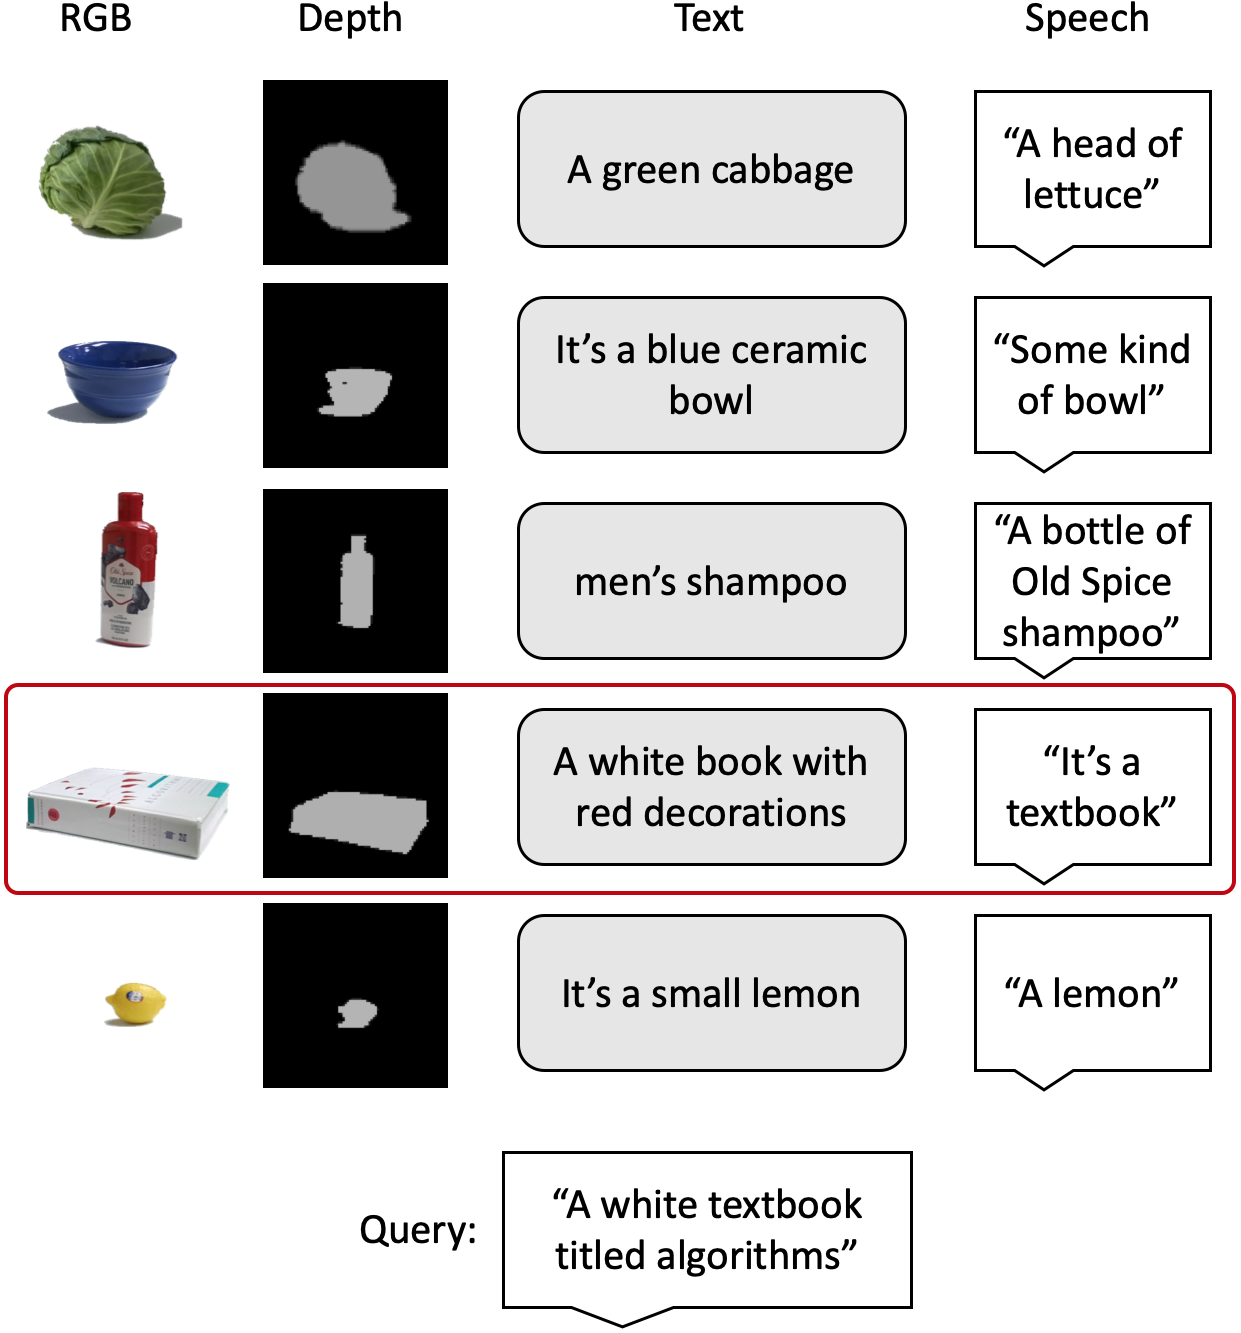
\includegraphics[width=.5\columnwidth]{Figures/experiment-setup.png}
\caption{
The experimental object retrieval setup, in which objects are represented by four modalities: an RGB image, a depth image, spoken descriptions, and textual descriptions. Given a query in some modality, our approach seeks to select the object that is the best fit, per a trained model. This approach, detailed in \cref{sec:Method}, is able to rank objects as to appropriateness even when one or more modalities is ablated at test time (e.g., depth inputs are missing), and outperforms state-of-the-art contrastive learning approaches on this task.
}
\label{fig:experimental-setup}
\end{figure}

More formally, we consider a spoken language command $x_s$, a textual language command $x_t$, a set of RGB images $X_r = \{x_r^{(1..n)}\}$, and a set of depth images $X_d = \{x_d^{(1..n)}\}$, the task is to retrieve the correct object by choosing the index that has the minimum distance from either of the language commands across all modalities.
Depending on which modalities are or are not ablated, we consider up-to four distances: ``sr,'' a vector of distances between $x_s$ and all RGB images in $X_r$; ``sd,'' a vector of distances between $x_s$ and all depth images in $X_d$; ``tr,'' a vector of distances between $x_t$ and all RGB images in $X_r$; and ``td,'' a vector of distances between $x_t$ and all depth images in $X_d$. In order to select the correct object, we first perform a component-wise average of the relevant modality pair distances for the available modalities. Then, we select the object which had the minimum distance, i.e., we perform an argmin on this average vector of multiple-modality distances. Depending on the missing/available sensors during test time, we might have any combination of these four distances. For example, if no written instructions are available at test time,\footnote{This setting is particularly salient. While large bodies of text are frequently available at training time, a person interacting directly with a physical agent may well prefer to use spoken instructions.} we compute the component-wise average of $sr$ and $sd$, and then select the object whose coordinate resulted in the lowest average distance. This method allows us to extend our model to support arbitrary modalities while remaining robust to test cases in which some modalities are missing or incomplete. 


%===================================================================

\section{Approach}
\label{sec:Method}

In keeping with previous work on the closely related problem of image retrieval, we focus on contrastive loss approaches, in which the goal is to learn an embedding of data where similar samples---in our case, samples belonging to the same class of object---are embedded `close' to one another, while dissimilar samples are farther apart. We develop a novel geometric loss function that simultaneously minimizes intra-class distances and maximizes inter-class distances across each pair of modalities yielding a model that is both effective at the retrieval task defined above and robust to modality dropouts at test time. We take an additional step and combine this geometric loss with a classification-based (cross-entropy) loss function which results in a superior model compared to either of geometric or cross-entropy losses alone.

\subsection{Geometric Alignment Loss}
\label{ssec:distanceloss}

% For $M$ modalities, we 
We define a distance-based loss function which can be used for arbitrary number of modalities. Our proposed method is inspired by the well-known similarity-based triplet loss~\cite{Carvalho-cooking-triplet,triplet_loss_2021_CVPR}, and is similar to contrastive loss~\cite{chen2020simple,NEURIPS2020_supervised_contrastive} under some settings.
Triplet loss-based learning works by forcing similar concepts from different domains `together' in some shared embedding space, while forcing dissimilar concepts `apart.' It is so named because it relies on three data points from the training set: a positive, a negative, and an anchor point. 
However, standard triplet loss cannot be used for more than two modalities. Therefore, we modify this concept as follows. During training, we sample two different instances and their corresponding representations from all modalities into two sets---one positive set (referring to a specific object) and one negative set (referring to some different object) as shown in \cref{fig:emma-loss}.
Unlike some prior triplet loss methods~\cite{GoLD_UMBC,triplet_loss_2021_CVPR}, the anchor is not randomly chosen from different modalities in each batch. Instead, in our setting, every item in the positive set becomes anchor once, and we minimize the distance between that item and other items in the positive set, while minimizing the distance between that item and all items in the negative set. It can be seen as an one-to-many relationship instead of an one-to-two relationship in the triplet loss formulation.
% the anchor and positive items are from the same object class, but in different modalities and each of the positives modalities becomes anchor once. 
We consider the following terminology:
% \todokdinline{I feel like using the terminology of triplet loss especially \textbf{anchor} is confusing here or maybe it needs to be rephrased. We can alternatively say that we consider all pairwise distances.}
% \todoffinline{I don't see the problem with anchor, but if you'd rather use a different term, what about query? As a note, while you do consider all pairwise distances but you treat some differently than others.}
\begin{itemize}
    % \item data point: a row in the csv/tsv file.
    \item Positive (Instance): A set of embeddings of one data point (e.g., an RGB image of an apple, corresponding depth image, text description, and speech description of the same apple)
    \item Negative (Instance): A set of embeddings of another data point of a different object (e.g., an RGB image of a book, corresponding depth image, text description, and speech description of the same book)
    \item Anchor (Modality): Every modality of the positive set is chosen as the learning anchor once. In our formulation, anchor is a ``concept'' referring to the points in the positive sets rather than a single instance in itself.
    %For our experiments, text is used. 
    The anchor is used as the basis for learning distances between positive and negative samples.
    % variance of text is lower and clusters of different objects are more distinct compared to other modalities, therefore, it can train a better model.
    % where we don't minimize the distance between the pair of embeddings from all modalities of the same data point, and we don't maximize the distance between positive and negative datapoints of the same modality.
    % \todo{explain this better}
    % \todokd{I rephrased it. Good?}
\end{itemize}

The objective is then to first minimize the distance between each pair of positive points from heterogeneous modalities, and second, maximize the distance between each positive and negative points from all modalities.
%and finally minimize the distance between each pair of negative points from heterogeneous modalities.
% The objective is then to first minimize the distance between the anchor and each of the other positive points from heterogeneous modalities, and second, maximize the distance between the anchor and each of the negative points from all modalities.
%and finally, maximize the distance between positive and negative anchor points from the same modality. 
% When we minimize the distance between each pair of positives, and maximize the distance between each pair of modalities one from the positive set and one from the negative set, the model converges faster than \supcon{} while maintaining the same performance when we have all modalities and a little bit less than Supcon when we drop text. 
We refer to this approach as \geom{}, for extended multimodal alignment which is formulated in \cref{eq:full-emma}. An illustration of this loss function is provided in \cref{fig:emma-loss}.

% \begin{equation}\label{eq:full-emma}
%     L = \sum_{m_1=1}^{M} \left[ \sum_{m_2=1}^{M} \left[ \max (\cos(z_{m_1}^{+}, z_{m_2}^{-}),0) \right] + \sum_{m_3=m_1+1}^{M} \left[ 1 - \max(\cos(z_{m_1}^{+},z_{m_3}^{+}),0) \right] \right]
% \end{equation}
\begin{equation}\label{eq:full-emma}
    L = \sum_{m_1=1}^{M} \left[ \sum_{m_2=1}^{M} \left[ \max (\cos(z_{m_1}^{+}, z_{m_2}^{-}) -1 + \alpha,0) \right] + \sum_{m_3=m_1+1}^{M} \left[ \max(1 - \cos(z_{m_1}^{+},z_{m_3}^{+}),0) \right] \right]
\end{equation}

In \cref{eq:full-emma}, $M$ is the number of modalities, the superscripts $+$ and $-$ represent positive and negative objects, $\alpha$ represents enforced margin between each positive and negative points which we set to 0.4 for all modalities without tuning, and $z$ is the embedding we get by applying a mapping function $f$, which in our case is a neural network on our input data.
In other words, $z_m = f_m(x_m)$, where each modality $m$ has a specific model $f_m$ that is different from the models for other modalities. These models do not share their weights. The $\cos(\cdot)$ function is a measure of similarity, not distance, and that is why the signs are reversed. 

To measure distance in embedded space, we use cosine similarity between pairs of embeddings, i.e. we measure the cosine of the angle between embeddings. Cosine similarity is a good choice for high-dimensional data as it is bounded between -1 and 1. Other distance metrics, such as Euclidean distance, grow in value with respect to their dimensionality, resulting in a very large distances for data points. Cosine similarity is the opposite of distance, and we need to reverse the logic for maximization and minimization.

Altogether, our proposed \geom{} function contains 
$3M^2-M/2$ terms: 
$M(M-1)/2$ anchor-to-positive distance minimizations and $M^2$ anchor-to-negative distance maximizations.
%, and $M(M-1)/2$ \textcolor{red}{optional} negative-to-negative distance minimizations.
%1 positive-to-negative anchor distance maximization.
It is noteworthy that our training procedure does not perform any stochastic dropout of modalities to obtain test-time robustness to missing modalities. Moreover, our approach does not need to compute the distance between all items in the batch as opposed to \supcon{}~\cite{NEURIPS2020_supervised_contrastive}.

\begin{figure*}[tb]
\centering
% 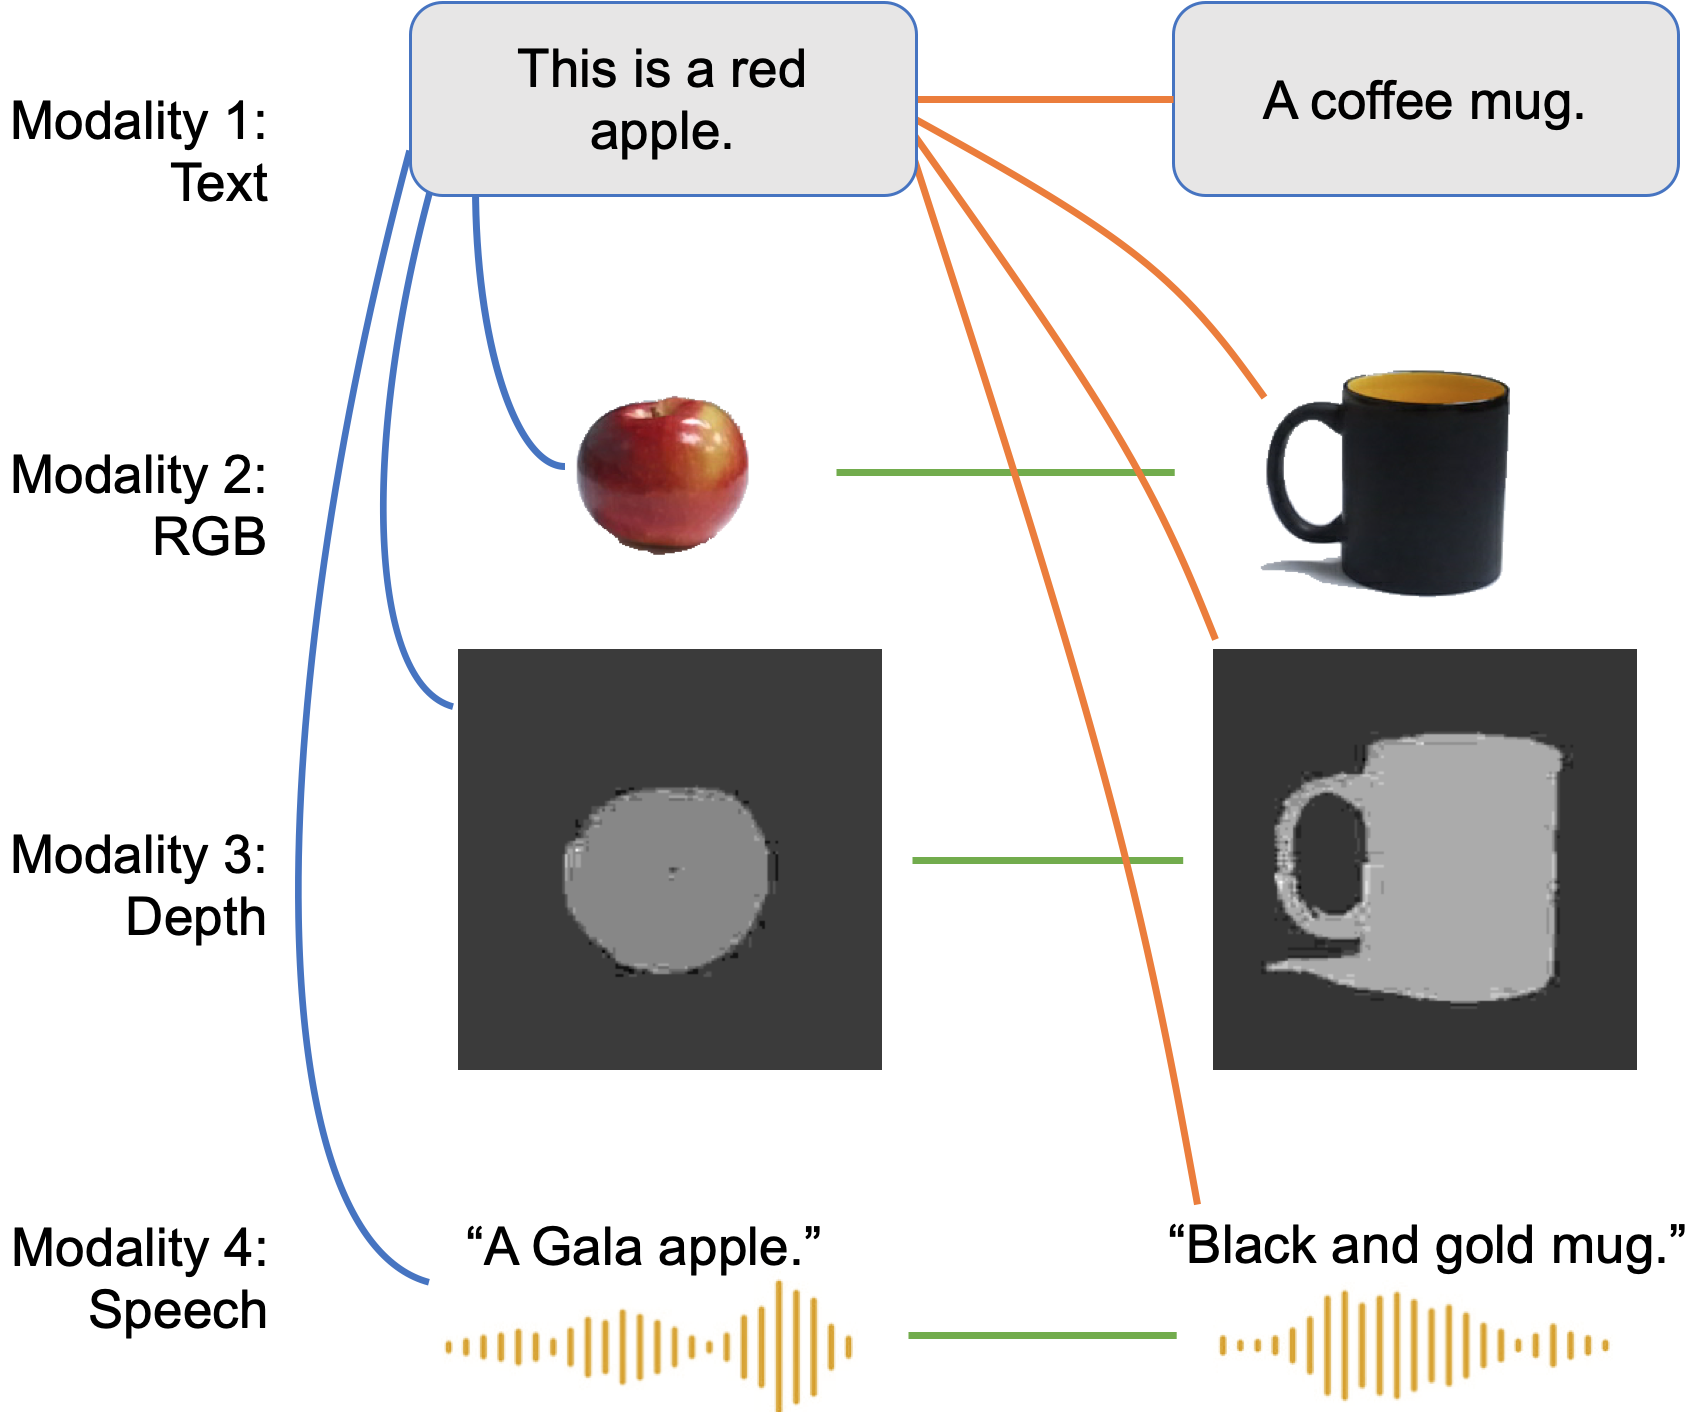
\includegraphics[width=.9\columnwidth]{Figures/4way-MMA.png}
% 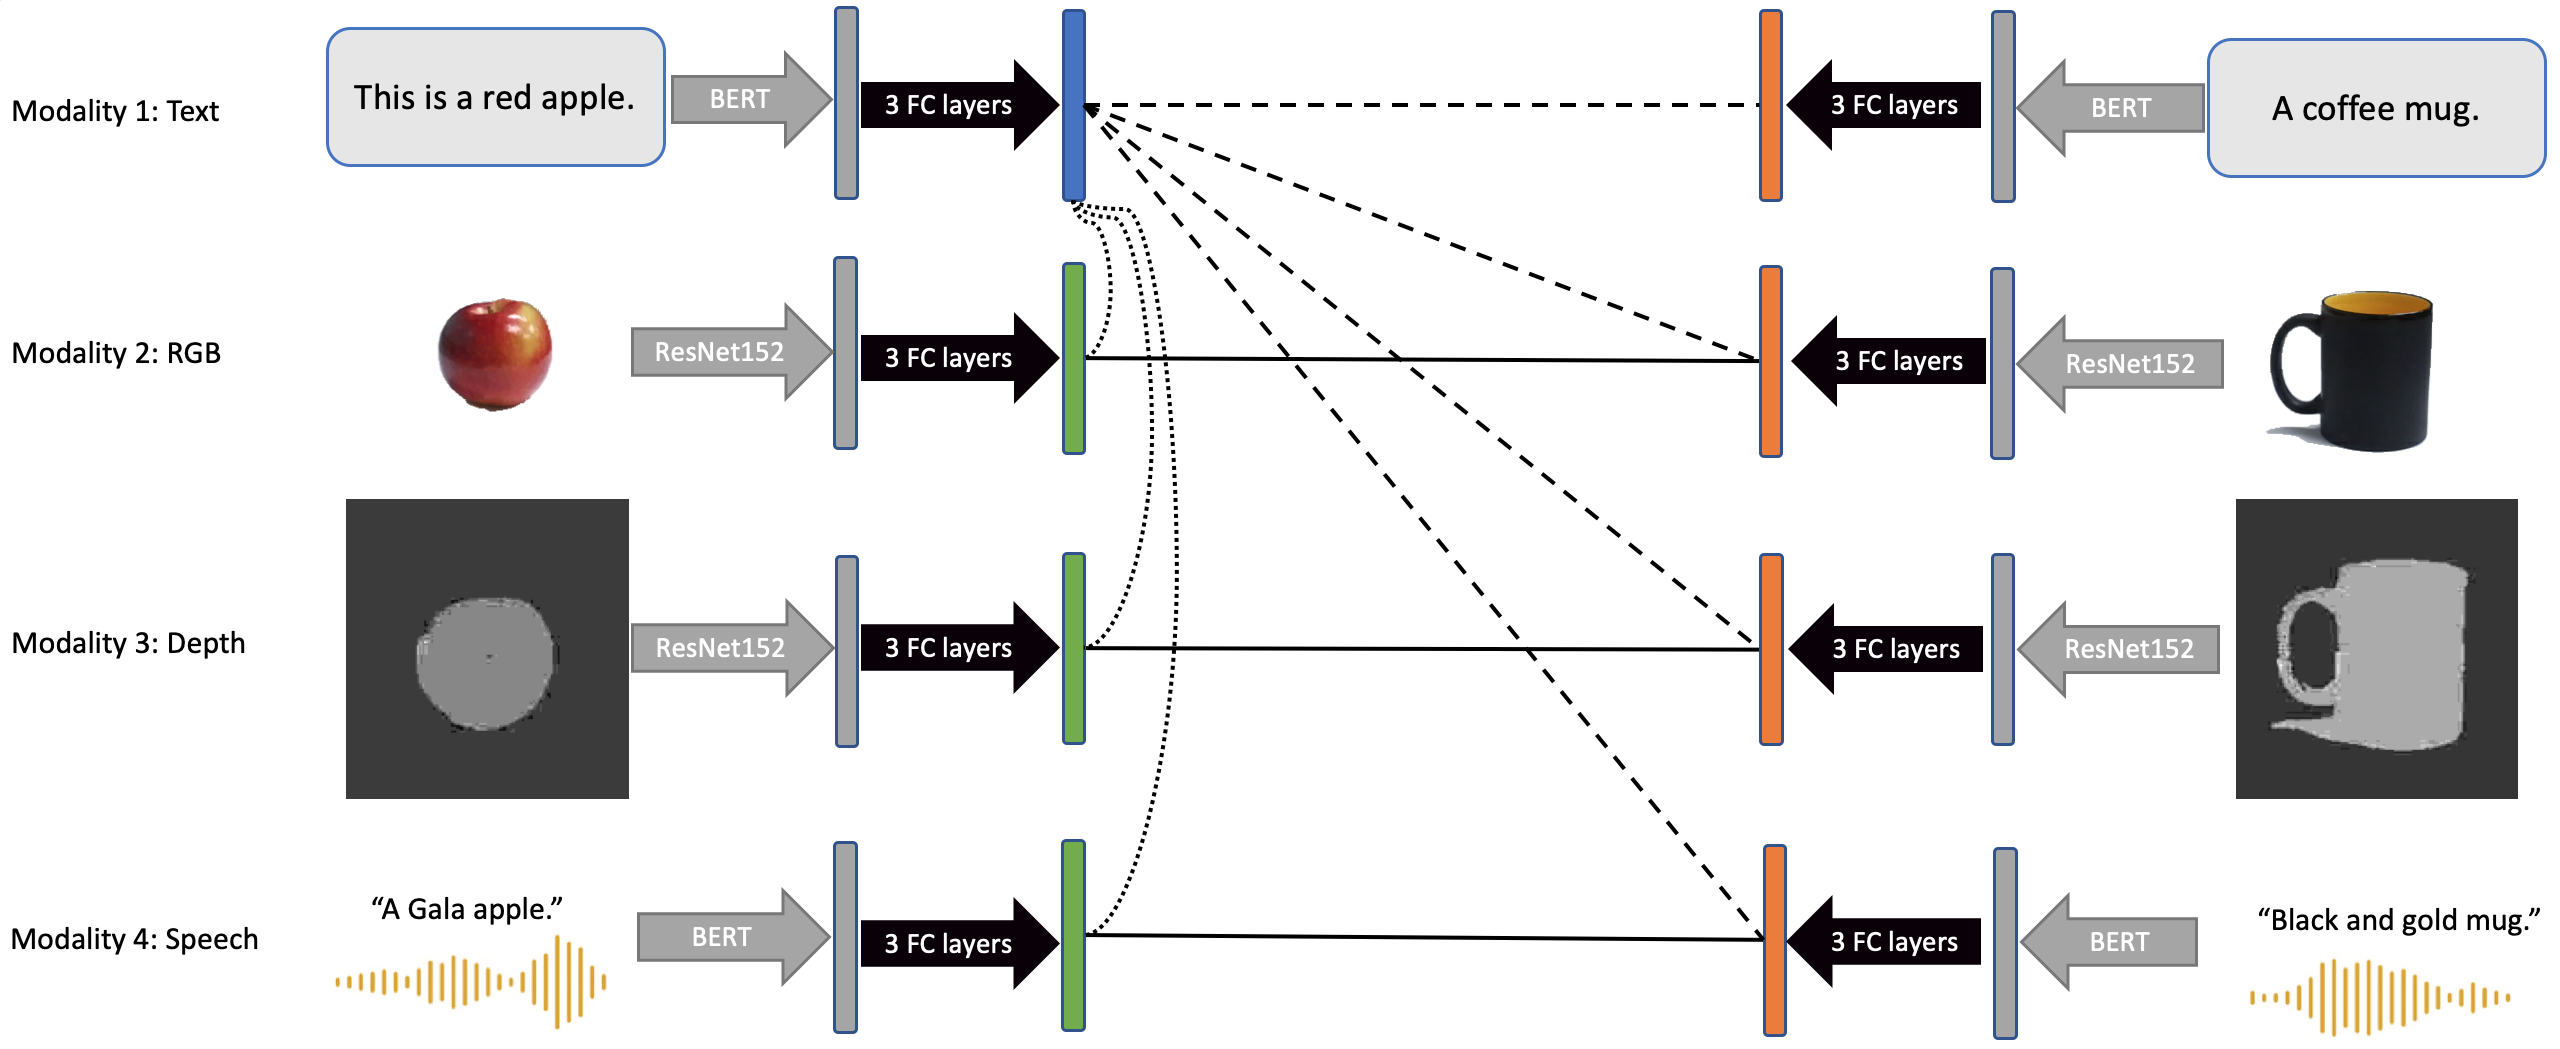
\includegraphics[width=2.1\columnwidth]{Figures/e-MMA.png}
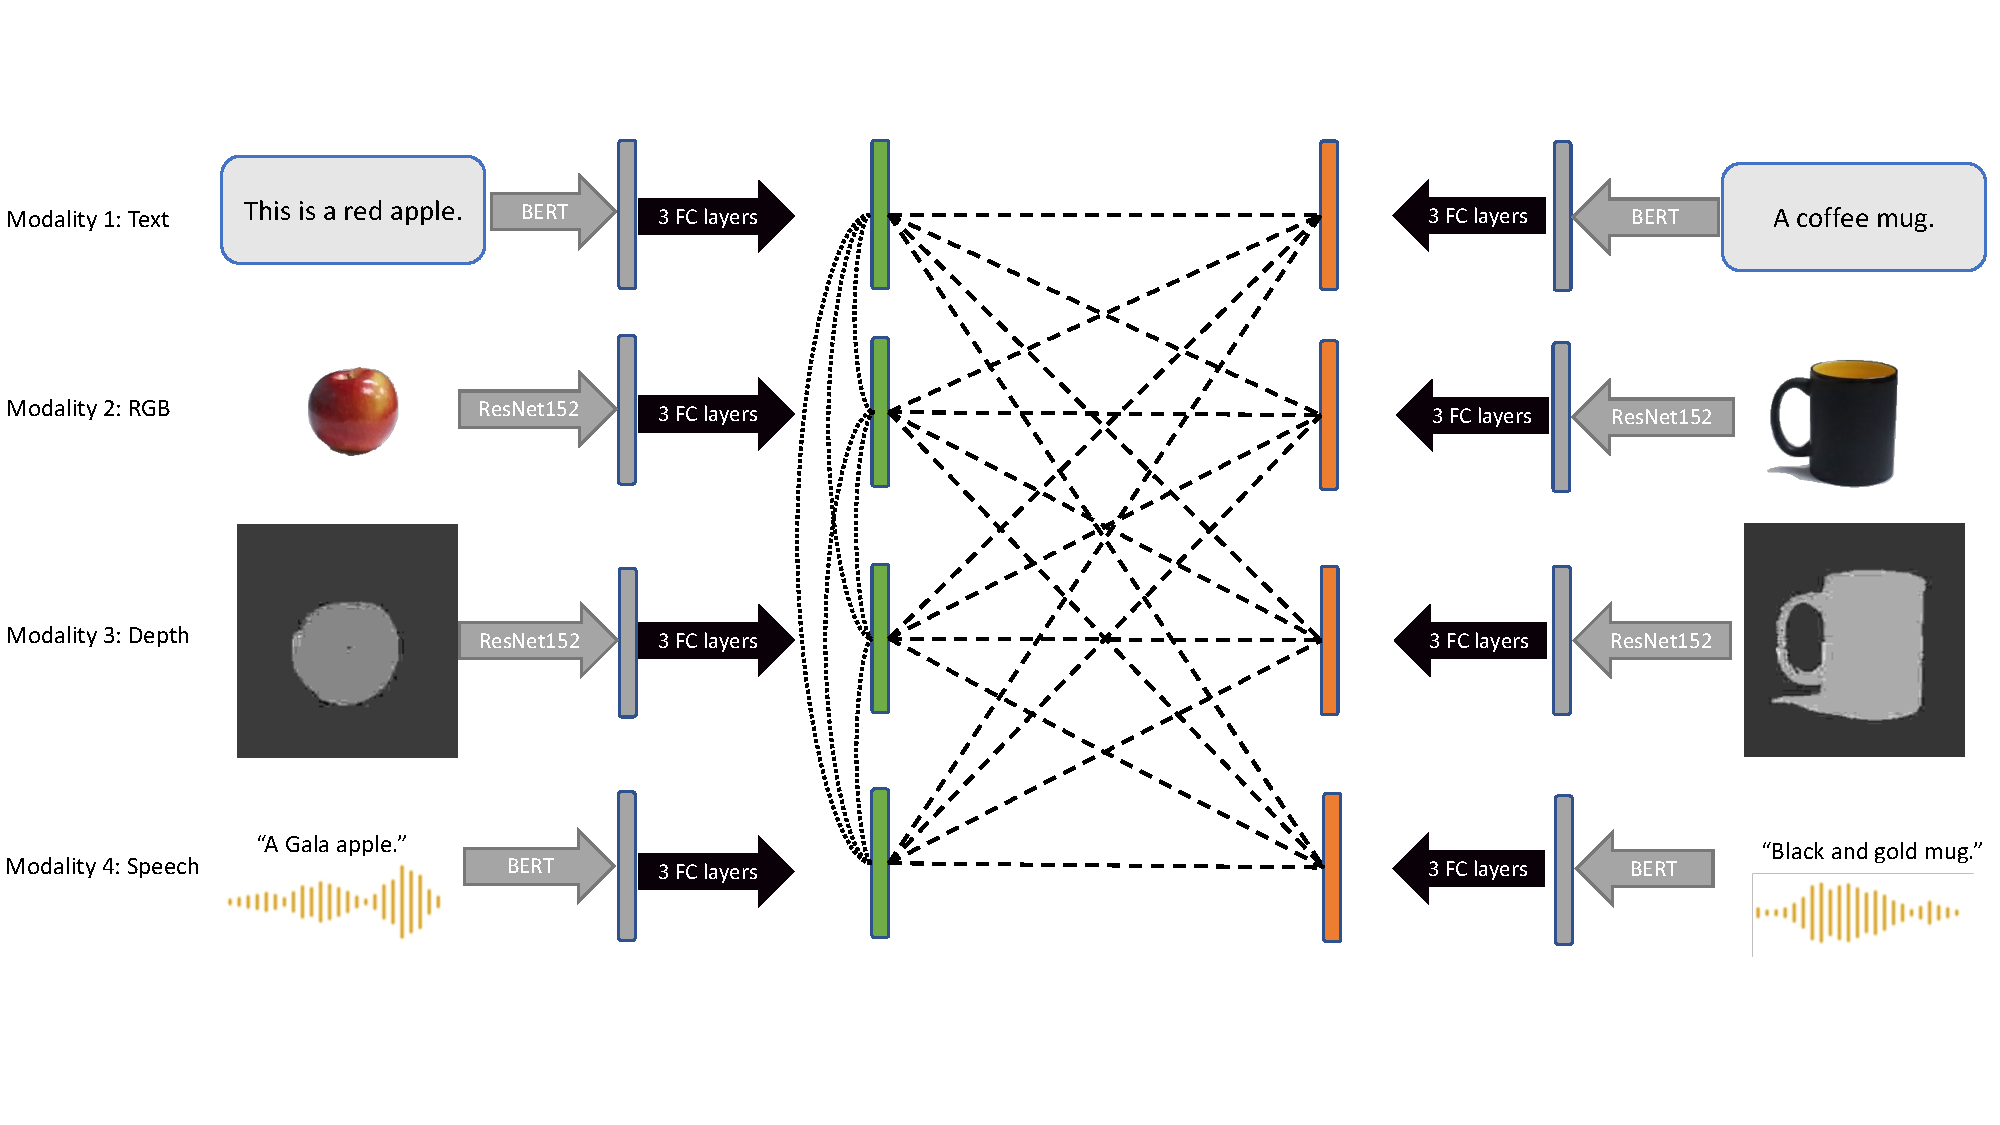
\includegraphics[width=1\columnwidth]{Figures/emma-loss.pdf}
\caption{A high-level prototype of our approach and the distances used in the \geom{} loss with four modalities. Gray arrows indicate pre-trained models that are frozen (i.e. the parameters are fixed and are not trained). The black arrows show 3 fully connected layers with a ReLU activitation function~\cite{relu2010} after the first two layers. These networks are trained.
Orange rectangles are negative embeddings and green rectangles are positive embeddings.
Dashed lines indicate distances to be maximized while dotted lines indicate distances to be minimized.%, and solid lines show the enforced margin.
}
\label{fig:emma-loss}
\end{figure*}




\subsection{Loss Development Story}
\todokdinline{Should I move this whole section to supplementary or should I talk about the high-level takeaways in the main paper?}

Our proposed loss function is a modification of the triplet loss function idea where we fix one modality as anchor and do not sample a positive instance from the same modality. 
Na\"ively, to extend triplet loss to work with arbitrary number of modalities, we can use two anchors (e.g., text and speech), which results in $2(M-2)$ triplet losses as formulated in~\cref{eq:objective-two-anchors}. 
\todoffinline{in this equation block, you're writing things like $|| z_{t}^{+} - z_{m}^{+} ||$. Do you actually mean norm, or would any old scoring function work?}
\todokdinline{This whole section will be moved to supplementary, but anyway, would it be better if I just get rid of the $||.||$ and use $\cos(x)$ instead?}

\begin{equation}
\label{eq:objective-two-anchors}
\begin{split}
    \mathcal{L}  &= \sum_{m=1}^{M-2} || z_{t}^{+} - z_{m}^{+} || - || z_{t}^{+} - z_{m}^{-} || + || z_{s}^{+} - z_{m}^{+} || - || z_{s}^{+} - z_{m}^{-} || \\
    &= \sum_{m=1}^{M-2} \cos(z_{t}^{+} ,z_{m}^{-}) - \cos(z_{t}^{+}, z_{m}^{+}) + \cos(z_{s}^{+} ,z_{m}^{-}) - \cos(z_{s}^{+}, z_{m}^{+})
\end{split}
\end{equation}

However, this approach performs poorly when one of the anchor modalities is ablated; since there is no explicit minimization between anchors, they do not necessarily map closely to each other, such that only one of the two anchors is actually learned. 


An alternative is to apply triplet loss $M-1$ times with a single anchor and $M-1$ `target' modalities.  In this case, the negative anchor point is disregarded. The positive anchor is used as an anchor for all $M-1$ triplet losses, and for each of those triplet losses the positive and negative points are simply selected from the corresponding modalities. \Cref{eq:objective-simple-mma} formulates this idea.

\begin{equation}
\label{eq:objective-simple-mma}
\begin{split}
    \mathcal{L}  &= \sum_{m=1}^{M-1} || z_{a}^{+} - z_{m}^{+} || - || z_{a}^{+} - z_{m}^{-} || \\
    &= \sum_{m=1}^{M-1} \cos(z_{a}^{+} ,z_{m}^{-}) - \cos(z_{a}^{+}, z_{m}^{+})
\end{split}
\end{equation}

However, this approach fails to take into account the dissimilarity of the positive and negative anchor points. This is an important piece of information that \cref{eq:objective-simple-mma} ignores. Although this information is implicitly captured when we maximize the distance between positive anchor and other negative modalities, when the negative data point becomes a positive example itself, the anchor and those points are forced to be closer to each other which can happen in three ways: either moving anchor closer to those points, moving those points closer to anchor, or move both somewhere in between. Therefore, in the last two cases we do not have explicit direct control over the distance between these points and previous positive points. Our experimental results confirm this hypothesis.

Therefore, we add an extra term which is responsible for maximizing the distance between positive and negative instances of the anchor modality, because a margin between positive and negative points from other modalities (excluding anchor) is enforced. 
% The first dashed line from the top in \cref{fig:emma-loss} is this extra term that captures the dissimilarity between positive and negative text datapoints.
We formulate this method in \cref{eq:objective-explicit-fixed-anchor}, which is generalized to an arbitrary number of modalities.

\begin{equation}
\label{eq:objective-explicit-fixed-anchor}
\begin{split}
    \mathcal{L}  %&= %\sum_{m=1}^{M-1} || z_{a}^{+} - z_{m}^{+} || - || z_{a}^{+} - z_{m}^{-} ||  - || z_{a}^{+} - z_{a}^{-} || \\
    &= \max(\cos(z_{a}^{+}, z_{a}^{-}) + \alpha_a, 0) + \sum_{m=1}^{M-1} \max \left(\cos(z_{a}^{+} ,z_{m}^{-}) - \cos(z_{a}^{+}, z_{m}^{+}) + \alpha_m, 0 \right) 
\end{split}
\end{equation}


In \cref{eq:objective-explicit-fixed-anchor}, $a$ represents the \textit{anchor} modality, $M$ is the number of modalities, the superscripts $+$ and $-$ represent positive and negative objects, $\alpha_m$ represents enforced margin for each modality which we set to 0.4 for all modalities without tuning, and $z$ is the embedding we get by applying a mapping function $f$, which in our case is a neural network on our input data.
In other words, $z_m = f_m(x_m)$, where each modality $m$ has a specific model $f_m$ that is different from the models for other modalities. These models do not share their weights. The $\cos(\cdot)$ function is a measure of similarity, not distance, and that is why the signs are reversed. 

Since the downstream task we are considering in the grounded language learning domain is to predict/retrieve a desired object among multiple objects given a natural language description, it makes sense to train the model using language as an anchor, and in fact anchoring learning around language outperforms anchoring on RGB. However, if use all modalities as anchor once (looping over modalities and compute distances between each pair), it results in a better performance.


% Triplet loss cannot be used for more than 2 modalities. Some previous work has concatenated RGB and depth embeddings to create a single ``vision'' embedding for learning~\cite{triplet_loss_2021_CVPR}, but they cannot handle RGB or depth sensor ablation during test. Since our method can handle any number of modalities, we can handle such a case by treating depth as a separate modality.
% Moreover, when using triplet loss with different anchors per batch, the batch size has to be 1 which makes training very slow.

% This approach is most similar to that of supervised contrastive learning~\cite{NEURIPS2020_supervised_contrastive}, but outperforms both that and regular contrastive learning~\cite{chen2020simple} methods when modalities are ablated, most notably written language.

% We find that the use of instance level losses grounded to one key modality (text) is sufficient to encourage a representation that satisfies our goals. 





\begin{comment}
\subsubsection{Extended Triplet}
Using an extended version of triplet loss to add all connections, which is formulated in \cref{eq:extended-triplet}, results in a worse performance.

\begin{equation}\label{eq:extended-triplet}
    L = \sum_{m_1=1}^{M} \left[ \sum_{m_2=m_1+1}^{M} \left[ \text{triplet}(z_{m_1}^{+}, z_{m_2}^{+}, z_{m_2}^{-}) + \text{triplet}(z_{m_1}^{-}, z_{m_2}^{-}, z_{m_2}^{+}) \right] + \cos(z_{m_1}^{+}, z_{m_1}^{-}) -1 + margin \right]
\end{equation}
Didn't change much when we drop text: Full eMMA when we have similar objects 

Did not work: Run the version with all connections (including among negatives) without triplet and just by using cosine distance between pair of embeddings
\end{comment}

\begin{comment}
\subsubsection{Smaller Batch Sizes}

Reducing the batch size from 64 to 16 (for both eMMA and supcon) increases the gap between our model and the baseline in cases where our model beats the baseline (all modalities, dropping speech), but baseline is still better than ours when we drop the text modality.

Batch size of 8 (for both eMMA and supcon) had a similar effect.

In batch size of 2 the trend is still the same, but when we drop the text modality, the MRR graph is flat on 0.4 which is still better than worse case and random case, but it seems model doesn't learn anything with regards to speech.
To remedy this, we add pulling connections among the modalities of the negative instance as formulated in \cref{eq:full-emma-pull-negatives} and as shown in \cref{fig:full-emma-pull-negatives}, and that solves the flatline problem when we drop the text modality, however, when we have all modalities it performs worse than formulation in \cref{eq:full-emma}.

\begin{equation}\label{eq:full-emma-pull-negatives}
\begin{split}
    L = & \sum_{m_1=1}^{M} \left[ \sum_{m_2=1}^{M} \left[ \max (\cos(z_{m_1}^{+}, z_{m_2}^{-}) -1 + margin,0) \right] + \sum_{m_3=m_1+1}^{M} \left[ \max(1 - \cos(z_{m_1}^{+},z_{m_3}^{+}),0) \right] \right. \\
    & \left. + \sum_{m_3=m_1+1}^{M} \left[ \max(1 - \cos(z_{m_1}^{-},z_{m_3}^{-}),0) \right] \right]
\end{split}
\end{equation}

\begin{figure*}[tb]
\centering
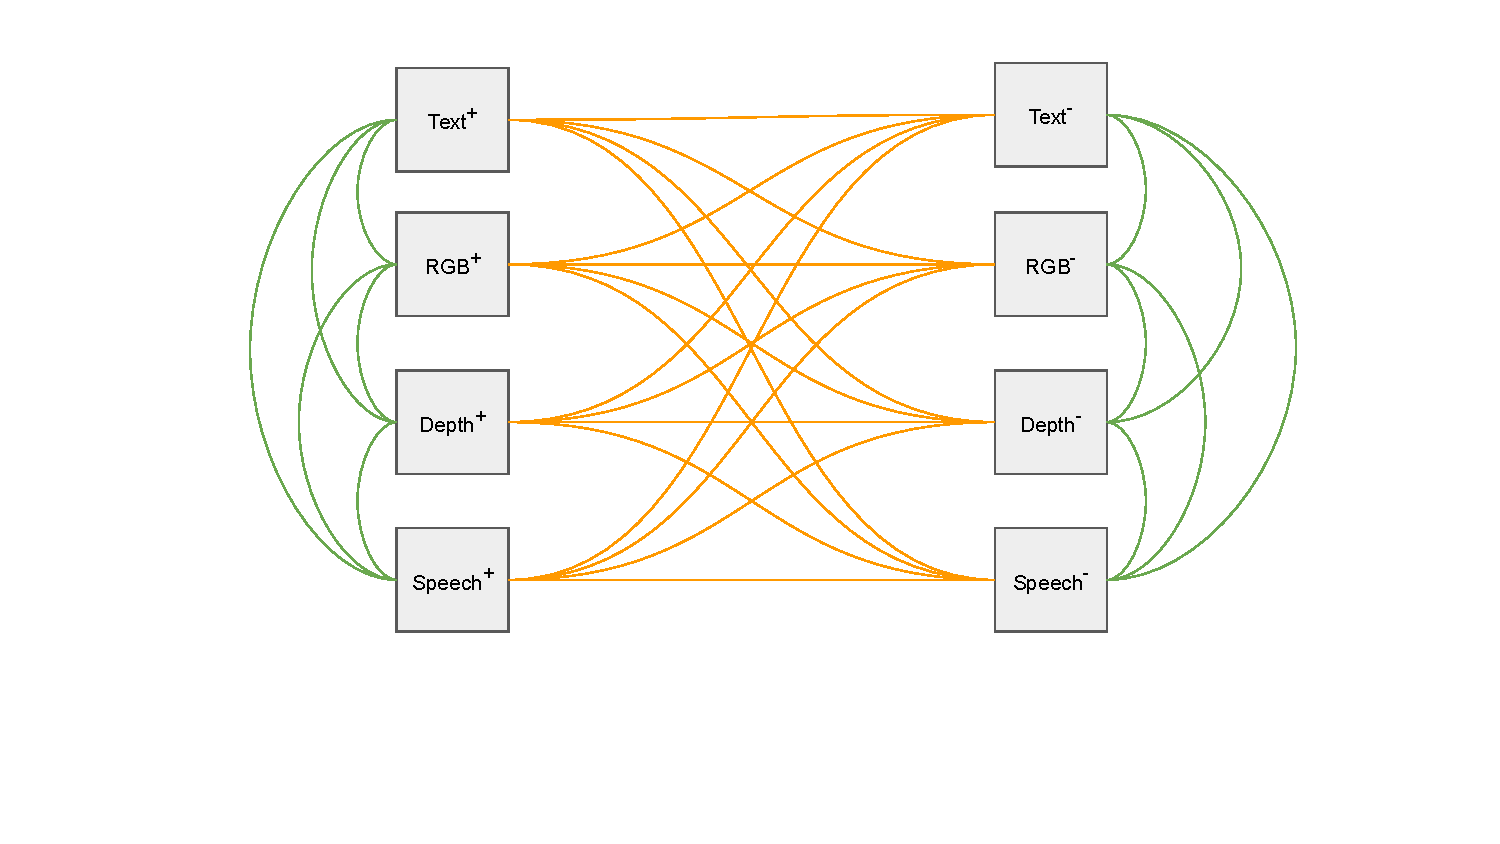
\includegraphics[width=1\columnwidth]{Figures/full-emma-pull-negatives.pdf}
\caption{A high-level prototype of our approach and the distances used when we have full EMMA and pulling among negatives}
\label{fig:full-emma-pull-negatives}
\end{figure*}
\end{comment}

\begin{comment}
\subsubsection{Margin}
% \todokdinline{Try different margins of 0.6, 1.0, and if it improved the results we can try to learn it as a parameter}
\todokdinline{Should we remove this section?}
I also tried two different margins so far. A margin of 0.6 and a margin of 1.0. Margin of 0.6 does not change the performance much. However, it converges even faster.
Margin of 1.0 (this is essentially just cosine similarity because we have: cos -1 +margin) results in a worse performance when we have all modalities. The MRR is 0.8995 when margin is 1, while with a margin of 0.6 the MRR is 0.9176, and with a margin of 0.4 the MRR is 0.9198.
If we drop the text modality, the MRR is 0.7923, 0.7913, and 0.6918 for margins of 0.4, 0.6, and 1.0 respectively.
\end{comment}


\subsection{EMMA: Extended Multimodal Alignment}
\label{sub:emma}

\todokdinline{We introduce \supcon{} in Baselines section which is after this section while we use SupCon as a part of our loss function here. Should we move the introduction of SupCon to here? Or maybe we can discuss the baselines first, and then Approach section follows it?}
\todocmi{I suggest a section 4.3, Baseline Approach: Supervised Contrastive Learning (pushing EMMA down)}

The main difference between \geom{} and \supcon{} is that in \geom{} we focus on the geometric interpretation of similarity using cosine distances, while in \supcon{}, cosine distances are used to compute a classification-based loss function similar to cross-entropy.
Both methods are valid and have some advantages that the other method does not offer. In \geom{}, the advantages are intuitive learning objective in terms of distance, interpretability of the learned embedding space, and faster convergence. 
The advantage of \supcon{} is that it uses classification objective which is aligned with the downstream task.

We propose to combine the \geom{} and \supcon{} and we refer to this approach as \ours{}, for extended multimodal alignment. \ours{} loss function is formulated in \cref{eq:emma}.

\begin{equation}\label{eq:emma}
    % \mathcal{L} = \geom{} + \supcon{}
    \ours{} = \geom{} + \supcon{}
\end{equation}

Combining these two losses results in faster convergence and better performance when we have all modalities available, and maintaining a good performance when modalities are missing.

\subsection{High-Level Findings/Observations}
We find that using each modality as anchor results in a better performance compared to when we fix one modality as anchor. This difference is more significant when we test with all modalities.

While the performance of SupCon deteriorates as the batch size is reduced, our \geom{} stays the same when we have all modalities or when we drop speech. However, when we drop text, EMMA deteriorate when we decrease batch size, and with a batch size of 2 without pulling negatives, it flatlines. In this case (when batch size is 2 and text is dropped), pulling among negatives is important and results in a better MRR.


We discuss the geometric interpretation of our method versus the classification interpretation of SupCon method and advantages of each.
Finally, we show that combining \geom{} with \supcon{} is superior to either the \geom{} approach or \supcon{} alone.


\begin{comment}
\subsubsection{EMMA + Binary Classification}
\todokdinline{Should we remove this section?}

When batch size is 64, it performs worse than baseline (SupCon) and EMMA itself. The experiment for the batch size of 2 also performs worse than other versions of EMMA, except for when we drop text.

There is a slight chance that I have made a mistake in my implementation of binary cross-entropy loss. My guesses (in decreasing order of likelihood) are:

1. The inputs to the BCE loss are $sigmoid(\cos_{sim}(z_i,z_j))$ for all $i \neq j$ where i is over the positive modalities only, while j is over both positive and negative modalities. Maybe I should've used $1-\cos(pos_i, pos_j)$ for similar embeddings and $cos(pos_i, neg_j) -1$ for dissimilar embeddings instead; similar to how EMMA's geometric loss is structured.

2. Let's assume $\text{predicts} = \text{sigmoid}(\cos_{sim}(z_i,z_j))$. Their corresponding labels/targets are 1 if i and j are from positive modalities, and 0 if j is from the negative modalities. The way I used PyTorch's BCE is that I passed the predicts whose targets are 1 to BCE first, passed the predicts whose targets are 0 to BCE in the next step, and finally added the two together. In other words:


\begin{equation}
\begin{aligned}    
loss &= 0.0 \\
loss &= loss + BCE(\text{similar predicts, targets}=1) \\
loss &= loss + BCE(\text{dissimilar predicts, targets}=0)
\end{aligned}
\end{equation}

Adding temperature gives mixed results; when we have all the modalities during the test, adding temperature improves performance over not having a temperature, but is still slightly worse than other methods. When we drop the text modality, however, the performance goes down.
\end{comment}

\subsection{Network Architecture}
\label{sec:Model}

Transformers are de facto architectures in natural language processing community and have shown great success across different tasks. Similar to~\citet{GoLD_UMBC}, we use BERT~\cite{devlin-etal-2019-bert} embeddings contained in the FLAIR library ~\cite{akbik2019flair,akbik-etal-2019-pooled} to featurize the textual input, and wav2vec2~\cite{wav2vec2} to extract audio embeddings from speech. Both of these encoders output a 3072-dimensional embedding vector which is generated by concatenating the last four hidden layers of their corresponding networks. Both BERT~\cite{devlin-etal-2019-bert} and wav2vec2~\cite{wav2vec2} are self-supervised language models using transformers~\cite{vaswani2017attention}.
% \todo[inline]{A couple of sentences about FLAIR and wav2vec2 and what they do}

To process images, we use ResNet152~\cite{He_resnet_2016} for both RGB and depth images which gives us a 2048-dimensional embedding vector. Depth images are colorized before passing to the ResNet152.

We then use different instantiations of the same multi-layer perceptron (MLP) consisting of 3 fully connected layers with ReLU activation~\cite{relu2010} to map each of these embeddings to a shared 1024-dimensional space where we can compute the distances between all embeddings. We note that these MLP networks are different and do not share any weights.




%===================================================================


\section{Experiments}
\label{sec:Experiments}

In this section we evaluate the quality of object retrieval models learned using the EMMA loss function. We first describe the dataset we use, give the metrics by which we evaluate the performance, the setup of the experiments, the baselines we compare against, and we end the section by a presenting results and analyzing them.

\subsection{Data}
\label{sec:Data}

We demonstrate the effectiveness of our approach on a recent publicly available multimodal dataset called GoLD~\cite{GoLD_UMBC}, which contains RGB image, depth image, written text descriptions, speech descriptions, and transcribed speech descriptions for 207 object instances across 47 object classes (see \cref{fig:emma-loss}). There are a total of 16,500 speech and 16,500 textual descriptions. The original GoLD paper uses raw RGB and raw depth images in which other objects are present in the background. We use a masked version of the images where the background is deleted (we observe that a masked version converges faster, however, they both converge to the same performance). Speech is converted to 16 Hz to match the wav2vec2 speech model~\cite{wav2vec2}.


\subsection{Setup and Metrics}
\label{sec:setupmetrics}
To evaluate our model we measure different performance metrics on a retrieval task where the model has to select an object among 5 objects given a language description. Only one of the objects corresponds to the description and the rest are from different object classes (e.g., one apple among a set including a fork, a mug, a lemon, and a bell pepper).


\subsubsection{Setup}
\label{sec:setup}
Similar to~\citet{NEURIPS2020_supervised_contrastive}, we use a stochastic gradient descent (SGD) optimizer with momentum~\cite{ruder2016overviewSGD} with a flexible learning rate starting at 0.05. 
% For the triplet loss experiments we use the Adam~\cite{kingma_adam_2015} optimizer with scheduling learning rate as suggested by the papers.
All models are trained for 200 epochs with a batch size of 64 on a Quadro RTX 8000 GPU.


To evaluate the performance, we compute the distance between the given natural language description and 5 randomly selected images (1 of which corresponds to the description, with the others from different object classes). We compute the distance between one language embedding and all candidate RGB embeddings, and we compute the distance between the same language embedding and all candidate depth embeddings corresponding to the RGB embeddings. We then take average of these two distance matrices. Instead of choosing an empirical threshold beyond which objects are considered to be `referred to,' we choose the closest image embedding (average distance of RGB and/or depth from language) as the prediction.
In order to use cosine \textit{distance}, we have to subtract the cosine of the \textit{angle} between two embeddings (which represents similarity) from 1: that is, we compute $1 - \cos(e_1, e_2)$.

\subsubsection{Metrics}
\label{sec:metrics}
The best metric to capture the performance in such a scenario is mean reciprocal rank (MRR, \cref{eq:mrr} for $Q$ queries). For each query we predict the rank of all objects based on their distance from the language command, and then the inverse rank of the desired objects in all queries are averaged. For example, if the model predicts the desired object as the first rank, then MRR = $\frac{1}{1} = 1$ which means a perfect score, and if it predicts the correct object as the last rank among five objects, then MRR = $\frac{1}{5}=0.2$. 

\begin{equation} \label{eq:mrr}
    \mathrm{MRR}=\frac{1}{|Q|} \sum_{i=1}^{|Q|} \frac{1}{\operatorname{rank}_{i}}
\end{equation}

Accuracy and micro F1 score
% (sklearn), flattened binary f1 score (sklearn), and F1 score 
are the same in this task, since for each prediction we either have a true positive and no false positives and no false negatives, or we have no true positives, one false positive and one false negative. MRR is a more informative metric because it captures the idea that having the correct object as the second choice should be considered better than having it as a last choice, while in accuracy the score is ``all or nothing''---either 0 or 1. Because our approach is designed to be robust to missing information across modalities, we also report MRR for different combinations of modality dropouts. 


\subsection{Baselines}
We compare both \ours{} and \geom{} against contrastive learning~\cite{chen2020simple} and supervised contrastive learning~\cite{NEURIPS2020_supervised_contrastive} which we refer to as \supcon{}.
We consider \supcon{} as the main baseline since it is a general version of multiple contrastive loss functions including triplet loss, the traditional version of contrastive loss usually used in self-supervised settings~\cite{chen2020simple}, and N-pair loss~\cite{NIPS2016N-PairLoss}.
% and do not include N-pair and triplet loss in our comparisons.
%contrastive learning methods including triplet loss, the traditional version of contrastive loss usually used in self-supervised settings~\cite{chen2020simple}, and supervised contrastive learning~\cite{NEURIPS2020_supervised_contrastive}. 



\begin{table*}[]
\centering
\resizebox{.97\textwidth}{!}{
\begin{tabular}{lc|ll|lll}
\multicolumn{1}{c}{} &  & \multicolumn{2}{c|}{\textbf{Accuracy}} & \multicolumn{3}{c}{\textbf{Mean Reciprocal Rank}} \\ \hline
\multicolumn{1}{c|}{\textbf{Method}} & \textbf{Modalities} & \multicolumn{1}{c|}{\textbf{\begin{tabular}[c]{@{}c@{}}Speech/RGB/\\ Depth\end{tabular}}} & \multicolumn{1}{c|}{\textbf{\begin{tabular}[c]{@{}c@{}}Text/RGB/\\ Depth\end{tabular}}} & \multicolumn{1}{c|}{\textbf{\begin{tabular}[c]{@{}c@{}}Speech/RGB/\\ Depth\end{tabular}}} & \multicolumn{1}{c|}{\textbf{\begin{tabular}[c]{@{}c@{}}Text/RGB/\\ Depth\end{tabular}}} & \multicolumn{1}{c}{\textbf{\begin{tabular}[c]{@{}c@{}}Text/Speech/\\ RGB/Depth\end{tabular}}} \\ \hline
\multicolumn{1}{l|}{EMMA} & TSRD & \multicolumn{1}{l|}{\textbf{0.65}$\pm$0.01} & 0.83$\pm$0.006 & \multicolumn{1}{l|}{\textbf{0.79}$\pm$0.002} & \multicolumn{1}{l|}{0.90$\pm$0.003} & 0.90$\pm$0.004 \\
\multicolumn{1}{l|}{EMMA} & 3 & \multicolumn{1}{l|}{--} & 0.84$\pm$0.008 & \multicolumn{1}{l|}{--} & \multicolumn{1}{l|}{0.90$\pm$0.004} & -- \\
\multicolumn{1}{l|}{\supcon{}} & TSRD & \multicolumn{1}{l|}{0.59$\pm$0.007} & 0.84$\pm$0.008 & \multicolumn{1}{l|}{0.75$\pm$0.004} & \multicolumn{1}{l|}{0.91$\pm$0.006} & 0.90$\pm$0.006 \\
\multicolumn{1}{l|}{\supcon{}} & 3 & \multicolumn{1}{l|}{--} & 0.84$\pm$0.006 & \multicolumn{1}{l|}{--} & \multicolumn{1}{l|}{0.91$\pm$0.004} & -- \\
\multicolumn{1}{l|}{Contrastive Cosine} & TSRD & \multicolumn{1}{l|}{0.40$\pm$0.153} & 0.83$\pm$0.006 & \multicolumn{1}{l|}{0.62$\pm$0.034} & \multicolumn{1}{l|}{0.90$\pm$0.004} & 0.89$\pm$0.005 \\
\multicolumn{1}{l|}{Contrastive Cosine} & 3 & \multicolumn{1}{l|}{--} & 0.84$\pm$0.005 & \multicolumn{1}{l|}{--} & \multicolumn{1}{l|}{0.91$\pm$0.003} & -- \\
\multicolumn{1}{l|}{\ours{}} & TSRD & \multicolumn{1}{l|}{--} & 0.83$\pm$0.008 & \multicolumn{1}{l|}{--} & \multicolumn{1}{l|}{0.90$\pm$0.005} & -- \\ \hline
\end{tabular}
}
\caption{Average and standard deviation of accuracy and MRR over 3 runs with 3 different random seeds on a held-out test set. These results represent performance when no modalities are ablated, in which case supervised contrastive loss, contrastive loss, and EMMA perform similarly (``--'' is an ablated modality and can't be evaluated). All metrics are from 0 to 1, and higher is better. For 5 objects, a random guess would have MRR of 0.33, and the worst case performance would be always ranking the correct item last which gives us 0.2. All models are trained using text as anchor. The batch size is 64 and optimizer is SGD for all experiments except the triplet loss, where batch size is 1 and optimizer is Adam. 
%In the Triplet experiment, RGB and Depth embeddings are concatenated to form a single vision embedding since triplet loss cannot be used for more than two modalities.
\todokdinline{Should we keep Acc or is MRR enough since table is out of bounds? Also, should we include other training modalities in the table? I inserted the results in a file called results-table.tex for now so that we can decide later.}
}
\todocmi{Let's include everything, and play tricks to shrink the table horizontally. If necessary it can be split into two tables with the same y headers and different x headers.}
\todoffinline{I've added a resizebox in order to get this to fit. This is not the desired solution (though currently the text isn't that small, so it could be okay) but I needed to see the entire table easily.}
\label{table:quantitative}
\end{table*}
% %Edward moved table above where refernced b/c LaTeX plays games with double-wide objects
% \begin{table*}[bth]
% \centering
% \begin{tabular}{c|c|c|c|c|c|c}
% \toprule
% \textbf{Method} & \textbf{Modalities} & \textbf{acc.srd} & \textbf{acc.trd} & \textbf{MRR.srd} & \textbf{MRR.trd} & \textbf{MRR.tsrd} \\ %\hline
% \midrule
% EMMA (Text) & 4 & \textbf{0.65}$\pm$0.01 & 0.83$\pm$0.006 & \textbf{0.79}$\pm$0.002 & 0.90$\pm$0.003 & 0.90$\pm$0.004 \\
% EMMA (Text) & 3 & - & 0.84$\pm$0.008 & - & 0.90$\pm$0.004 & - \\
% % Simple MMA (Text)  & 3 & ?$\pm$? & ?$\pm$? & ? & ? \\
% % Simple MMA (Text) & 4 & ?$\pm$? & ?$\pm$? & ? & ? \\
% % Simple MMA (Speech) & 3 & ?$\pm$? & ?$\pm$? & ? & ?  \\
% DONE Supervised Contrastive (Text)& 4 & 0.59$\pm$0.007 & 0.84$\pm$0.008 & 0.75$\pm$0.004 & 0.91$\pm$0.006 & 0.90$\pm$0.006  \\
% TODO Supervised Contrastive (Text)& 3 & - & 0.84$\pm$0.006 & - & 0.91$\pm$0.004 & -\\
% DONE Contrastive Cosine (Text) & 4 & 0.40$\pm$0.153 & 0.83$\pm$0.006 & 0.62$\pm$0.034  & 0.90$\pm$0.004 & 0.89$\pm$0.005\\
% TODO Contrastive Cosine (Text) & 3 & - & 0.84$\pm$0.005 & -  & 0.91$\pm$0.003 & -\\
% PROJ Triplet (Text) & 3 & - & 0.83$\pm$0.008 & - & 0.90$\pm$0.005 & -  \\
% % DONE EMMA (Speech) & 3 & ?$\pm$? & ?$\pm$? & - & - \\
% % DONE EMMA (Speech) & 4 & ?$\pm$? & ?$\pm$? & ? & ? \\
% % DONE Supervised Contrastive (Speech)& 3 & ?$\pm$? & ?$\pm$? & - & -\\
% % DONE Supervised Contrastive (Speech)& 4 & ?$\pm$? & ?$\pm$? & ? & ? \\
% % TODO Contrastive Cosine (Speech) & 3 & ?$\pm$? & ?$\pm$?  & - & -\\
% % TODO Contrastive Cosine (Speech) & 4 & ?$\pm$? & ?$\pm$?  & ? & ?\\
% % DONE Triplet (Speech) & 3 & ?$\pm$? & ?$\pm$? & - & -  \\

% % Full MMA (Text) w/ neg & 3 & ?$\pm$? & ?$\pm$? \\
% % Simple MMA (Text) w/ neg Adam & 3  & 0.7949$\pm$? & 0.8778$\pm$? \\
% % Simple MMA (Text) w/ neg SGD & 3 & 0.7905$\pm$? & 0.8821$\pm$? \\
% % Triplet (Text) w/ neg & 3 & 0.7497$\pm$? & 0.8522$\pm$? \\
% % Full MMA (Speech) w/ neg & 3 & ?$\pm$? & ?$\pm$? \\
% % Simple MMA (Speech) w/ neg & 3 & 0.7949$\pm$? & 0.8778$\pm$? \\
% % Contrastive Cosine (Text) w/ neg & 3 & 0.7894$\pm$? & 0.8788$\pm$?  & ? & ?\\
% % Contrastive (Speech) w/ neg & 3 & ?$\pm$? & ?$\pm$? \\
% % Triplet (Speech) w/ neg & 3 & 0.7497$\pm$? & 0.8522$\pm$? \\
% \bottomrule
% \end{tabular}
% \caption{\label{table:quantitative}Average and standard deviation of accuracy and MRR over 3 runs with 3 different random seeds on a held-out test set. These results represent performance when no modalities are ablated, in which case supervised contrastive loss, contrastive loss, and EMMA perform similarly. All metrics are from 0 to 1, and higher is better. For 5 objects, a random guess would have MRR of 0.33, and the worst case performance would be always ranking the correct item last which gives us 0.2. All models are trained using text as anchor. The batch size is 64 and optimizer is SGD for all experiments except the triplet loss, where batch size is 1 and optimizer is Adam.
% % \todokdinline{maybe adding results on cropped and raw dataset as well. Also results using object class instead of negative sampling}
% }
% \end{table*}


\subsubsection{Triplet Loss}
\label{sub:baseline-triplet}
\todokdinline{Since we do not include triplet in our analysis, it might make more sense to move this section into the introduction of Approach to motivate why we came up with EMMA, thoughts?}

The triplet loss function consists of three data points including anchor, positive, and negative from two modalities. The anchor, positive, and negative can be chosen from different modalities in each batch.
The major disadvantage of the triplet loss method is that it cannot be used for more than two modalities. 
%Second, a batch size of greater than 1 is hard to implement if the anchor, positive, and negative come from different modalities for each batch.
% To address these issues in EMMA, we sample more than one positive and negative data points.
\todokd{If moved to approach section, build on this to introduce our geometric loss function.}
To address this issue, in \geom{} we use pairwise distance optimization for all data points. 
%Intuitively, we sample one positive data point and one negative data point, each of which includes $M$ modalities, resulting in 2M data points. Each of the $M$ positives modalities become an anchor once. 
% \Cref{table:quantitative} shows that our MMA method perform as good as this baseline while our model can be trained 10x faster since we can use batch sizes larger than 1. Also, 
Our method can be used for any number of modalities, while previous works that use triplet loss~\cite{GoLD_UMBC,triplet_loss_2021_CVPR} concatenate RGB and depth to form a single ``vision'' vector to handle three modalities, but they cannot handle RGB or depth sensor ablation during test. Since our method can handle any number of modalities, we can handle such a case by treating depth as a separate modality.
Moreover, our method has the advantage that does not require triplet mining or providing hard negative examples.
% When we used a fixed anchor modality, a batch size of 64, and applied semantic negative sampling~\cite{Pillai_Matuszek_2018}, our method outperformed this baseline. However, 
Since this method cannot be applied to four modalities, we do not include it in the main analysis. 

\subsubsection{Contrastive Loss}
\label{sub:baseline-contrastive}


We compare our model against contrastive learning method presented by~\citet{chen2020simple} where they use the normalized
temperature-scaled cross entropy loss (NT-Xent). In order to implement this loss function, we use cosine similarity as suggested in the SimCLR paper~\cite{chen2020simple}. Another possibility is to use an inner dot product~\cite{NEURIPS2020_supervised_contrastive}; if not normalized, this can lead to numerical instabilities and overflow/underflow since the dot product is not bounded, but the result is the same whether we use normalized inner dot product or cosine similarity. Contrastive loss function is formulated in \cref{eq:contrastive-loss}:
% \todokdinline{try contrastive loss with cross-entropy, dot product, and the supervised contrastive method itself (without triplets).}

% Original Formula
\begin{equation}\label{eq:contrastive-loss}
    -\sum_{i \in I} \log \frac{\exp (sim(z_i , z_{j(i)}) / \tau) }{\sum_{a \in A(i)} \exp (sim(z_i, z_a) / \tau)}
\end{equation}
% \begin{equation}\label{eq:contrastive-loss}
%     -\sum_{i \in I} \log \frac{\exp (sim(f(x_i) , z_{j(i)}) / \tau) }{\sum_{a \in A(i)} \exp (sim(f(x_i), f(x_a)) / \tau)}
% \end{equation}
where $i$ is anchor, $j(i)$ is the set of positives excluding anchor, $a$ is the set of all positives and negatives excluding anchor, and $z = f(x)$.

We can treat different modalities of the same instance as ``augmentations'' of that instance, and consider them as the positive points for the anchor.
\Cref{eq:contrastive-loss} can be rewritten with the sum over positives explicitly shown as formulated in \cref{eq:explicit-contrastive}.

%, which is equivalent to ``augmented views'' in the contrastive loss terminology.

\todokdinline{Notation for M - i, it should be something like other modalities of the anchor but it shouldn't be over number of modalities.}
\begin{equation}\label{eq:explicit-contrastive}
    - \sum_{i \in I} \sum_{p=1}^{M \setminus \{i\} } \log \frac{\exp (sim(z_i , z_{p})/ \tau) }{
    \sum_{a \in A(i)} \exp (sim(z_i, z_a) / \tau)}
    %{ \exp (sim(z_i^+ , z_{m}^{+}) / \tau) + \exp (sim(z_i^+, z_{m}^{-}) / \tau)}
\end{equation}
where $M$ is the number of modalities (e.g. RGB image, depth image, speech, text) and $z = f(x)$.


\subsubsection{Supervised Contrastive Learning}
\label{sub:baseline-supcon}

\citet{NEURIPS2020_supervised_contrastive} extend the contrastive learning method (NT-Xent) and propose a supervised way of performing contrastive learning to treat not only augmentations of the anchor, but also every item that shares the same label with anchor as positives. This loss function is shown in \cref{eq:supervised-contrastive}.

\begin{equation}\label{eq:supervised-contrastive}
    \sum_{i \in I} \frac{-1}{|P(i)|} \sum_{p \in P(i)} \log \frac{\exp (z_i \cdot z_p / \tau) }{\sum_{a \in A(i)} \exp (z_i \cdot z_a / \tau)}
\end{equation}

% \begin{equation}\label{eq:supervised-contrastive-my-notation}
%     \sum_{i \in I} \frac{-1}{|P(i)|} \sum_{p \in P(i)} \log \frac{\exp (f_i(x_i) \cdot f_p(x_p) / \tau) }{\sum_{a \in A(i)} \exp (f_i(x_i) \cdot f_a(x_a) / \tau)}
% \end{equation}

Although, this loss function do not use cosine similarity, they normalize the embeddings before performing dot product which is equivalent to cosine similarity.

The main difference between the contrastive loss baseline in \cref{sub:baseline-contrastive} and \supcon{} is that there is no notion of meaningful negative points in contrastive loss, and everything in the batch that is not the anchor or one of the positive views is considered to be negative. In \supcon{}, however, all elements in the batch that have same label as the anchor, are also considered positives in addition to different views of the same instance. While the denominators of \cref{eq:explicit-contrastive,eq:supervised-contrastive} stay the same, this subtle difference affects the numerator and includes more positive examples.

While this model is a strong baseline, the authors applied it to a unimodal dataset. In this paper we extend this baseline to work with a multimodal dataset and show that it is slower than \ours{} to learn and its performance is also lower when all modalities are available during test time.
% if modalities are ablated, this method does not perform as well as our proposed model (we show and discuss this later, in \cref{fig:epochs-mrr.srd}). This is especially true when the text modality is dropped, as is likely in physical agent scenarios, where speech is a natural interaction mechanism.


\subsection{Modality Ablation}
% \todokdinline{Should I remove this section altogether or should I just mention that our method is equal or better in all cases except when we drop text? Or should I spend more time to come up with something so that we can perform better than baseline even in this case?}
We consider an experiment in which we incorporate RGB, depth, speech, and written language to train the model. The loss function requires no changes beyond adjusting the value of $M$ in \cref{eq:full-emma} according to the number of modalities available during training. Our goal is the non-trivial downstream prediction task: determining what objects are being referred to by arbitrary language from a small number of examples. When we consider only text, RGB, and depth, written language is used as the query modality, and we compute the distance of RGB and depth modalities from it and then average them. However, when speech is incorporated as an additional fourth sensory modality, we have three possible choices. \textit{First}, we can compute the distance of RGB and depth from text and from speech which gives us 4 distance matrices, and then take average of these four. \textit{Second}, we can treat speech in a similar way to RGB and depth: compute the distance of RGB, depth, and speech from text, and then take an average of three of them. \textit{Third}, similar to the first method, but adding the distance between language and speech as well and then take the average of 5 distance matrices.

Of these, the first method is the most appropriate choice for a robust multimodal alignment approach. The second and third options are possible during training, but in real-world object retrieval scenarios, having only one form of language instructions is a reasonable scenario---people are not likely to \textit{both} speak about \textit{and} type in instructions for an agent. At test time, depending on which modalities are available to the model, we can use speech, text, or both to compute the distance of RGB and depth embeddings from the linguistic query, and then take the average.
\Cref{eq:distance-matrix} shows all possible cases of modality dropout and the corresponding distance computations, where ``t'' represents \textit{text}, ``s'' represents \textit{speech}, ``r'' represents \textit{RGB}, ``d'' represents \textit{depth}, $K_{ij}$ for each pair of modalities is the distance of one instance in modality $i$ from all candidate instances in modality $j$, and $K$ is the final distance---a matrix if there are multiple queries and a vector if there is one query.
\begin{equation}
\label{eq:distance-matrix}
K = 
    \begin{cases} 
        K_{tr} & \text{speech and depth are missing} \\
        K_{sr} & \text{text and depth are missing} \\
        K_{td} & \text{speech and RGB are missing} \\
        K_{sd} & \text{text and RGB are missing} \\
        K_{trd} = \frac{K_{tr} + K_{td} }{2} & \text{speech is missing} \\
        K_{srd} = \frac{K_{sr} + K_{sd} }{2} & \text{text is missing} \\
        K_{tsr} = \frac{K_{tr} + K_{sr} }{2} & \text{depth is missing} \\
        K_{tsd} = \frac{K_{td} + K_{sd} }{2} & \text{RGB is missing} \\
        K_{tsrd} = \frac{K_{tr} + K_{td} + K_{sr} + K_{sd} }{4} & \text{o.w.} \\
    \end{cases}
\end{equation}


\Cref{fig:epochs-mrr.lard,fig:epochs-mrr.srd,fig:epochs-mrr.ld,fig:epochs-mrr.lr} show the relative performance of \ours{} and \geom{} against baselines when different modalities are ablated.


\subsection{Results}
\label{sec:results}

In this section we provide quantitative and qualitative results by comparing our method against supervised contrastive learning~\cite{NEURIPS2020_supervised_contrastive} and na\"ive contrastive loss~\cite{chen2020simple}.
% We evaluate our EMMA loss function against the na\"ive triplet loss method. Our model significantly outperforms the triplet method across all epochs while it converges faster as shown in \cref{fig:epochs-mrr.srd}.
\Cref{table:quantitative} summarizes the performance of all models with different ablation metrics.
% \todo[inline]{Why do we call out triplet loss specifically? We evaluate against several baselines? I don't understand this section particularly}
To provide a better sense of the performance measure, we can think of a model that always ranks the correct object in the second place which is not very bad. Such a model would have MRR of $1/2 = 0.5$.

\Cref{fig:epochs-mrr.lard} Shows that \ours{} learns faster and results in a better performance compared to both \supcon{} and contrastive learning~\cite{chen2020simple} when trained using all modalities and all modalities are available during test. We observe that not only does contrastive loss learn more slowly, but that it is prone to overfitting; while this can be addressed with careful tuning of the learning process, it is better not to have to.

\begin{figure}[tbh]
\centering
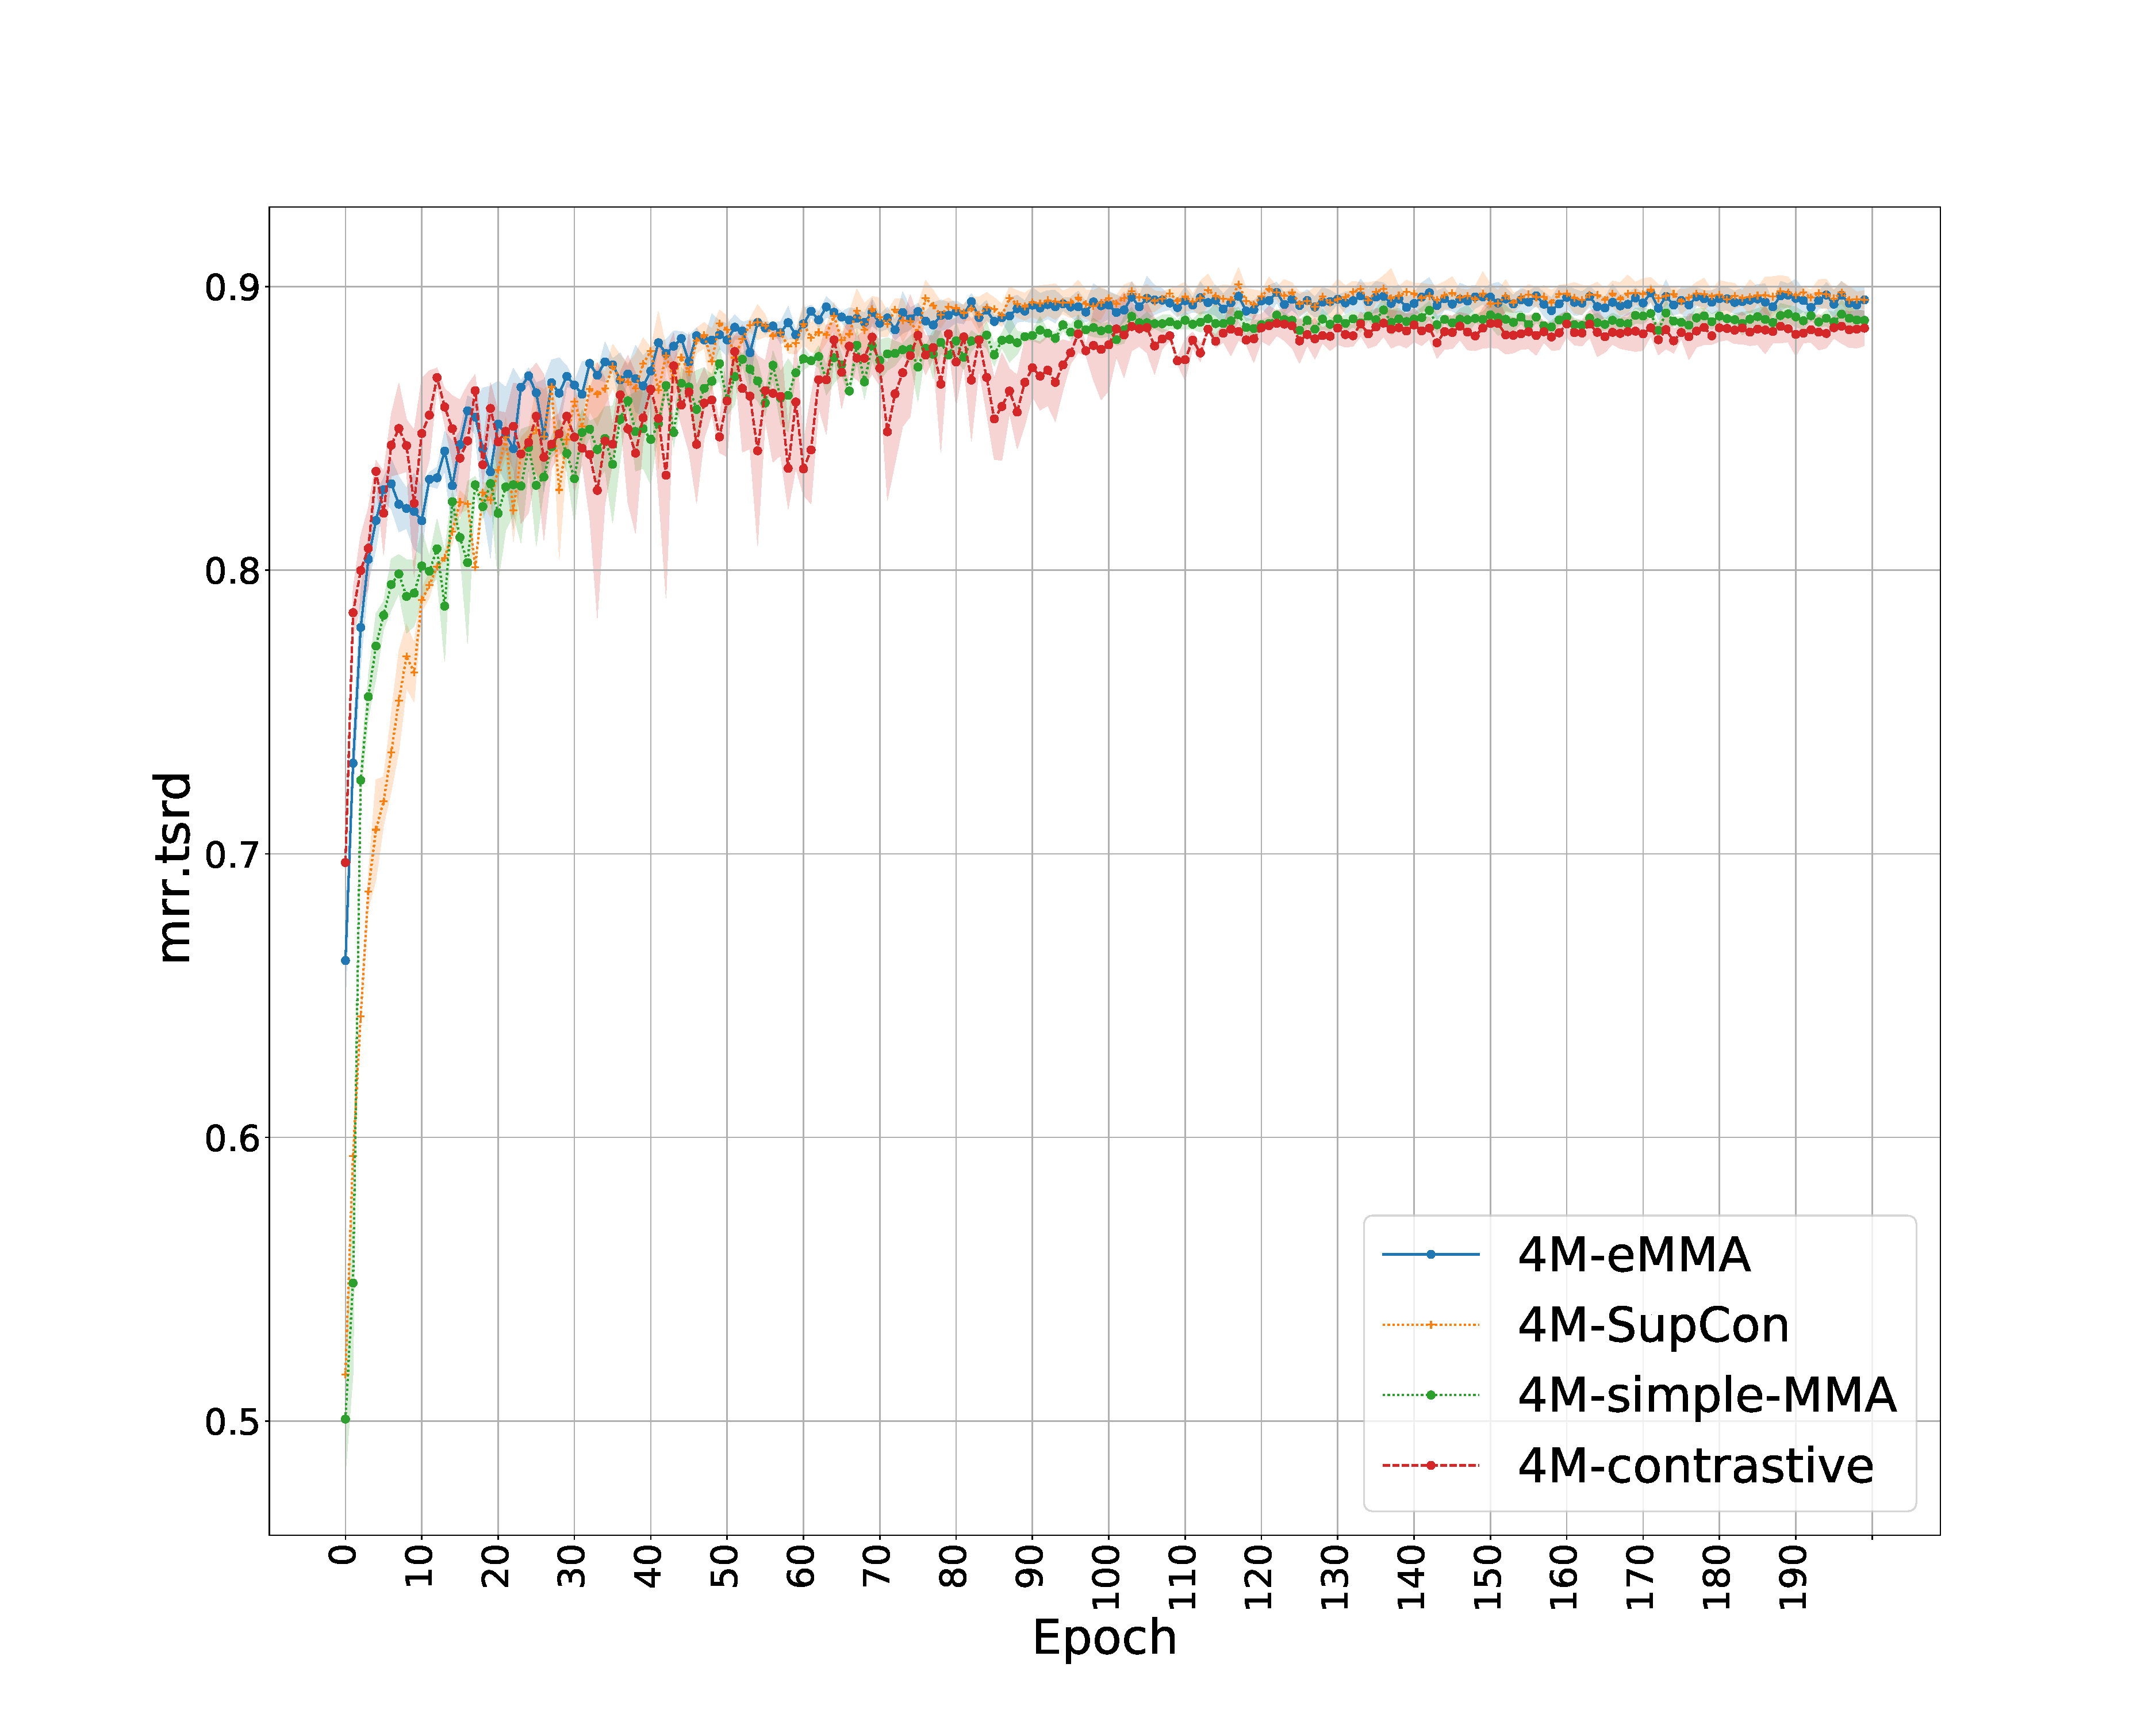
\includegraphics[width=.99\columnwidth]{Figures/average-seeds-epochs-mrr_lard}
\caption{Mean Reciprocal Rank (MRR) on the held-out test set when all modalities are available, averaged over 5 runs. Green is \ours{}, orange is \supcon{}, blue represents our \geom{} loss function, and red is the contrastive loss baseline. Higher is better.
}
\label{fig:epochs-mrr.lard}
\end{figure}


% Comparing \cref{fig:epochs-mrr.trd} and 
When we drop the text modality in \cref{fig:epochs-mrr.srd}, we can see that the performance decreases from about 0.93 to about 0.82, showing that speech cannot completely replace the text. \Cref{fig:3d-tsne} depicts that speech modality is not aligned as good as the text modality and that is why when we drop text and use speech as the main query, the performance decreases. This supports our hypothesis that a geometric alignment of the latent space is crucial to a good performance for object retrieval and multimodal understanding.
In \cref{fig:epochs-mrr.srd}, we observe that when speech is used as the query and text modality is ablated, \supcon{} baseline works slightly better than \ours{}, although \ours{} still learns faster. The reason is that \supcon{} optimizes for the classification task, and since the speech modality is not well aligned based on \cref{fig:3d-tsne}, using \geom{} makes the downstream task more difficult by trying to pull and push similar and dissimilar data points, respectively. More research needs to be done to come up with strategies to align more chaotic modalities.
% We also observe that speech has a higher variance compared to text, and a na\"ive contrastive learning method cannot take advantage of text modality to reduce this variance. While the other two methods leverage text modality to align speech better.

There is very little gap in performance when depth or RGB are dropped in \cref{fig:epochs-mrr.lr,fig:epochs-mrr.ld} compared to when we have all modalities in \cref{fig:epochs-mrr.lard} which shows that our model is robust enough when rgb or depth sensors fail in real-world deployment. Also, when depth is dropped in \cref{fig:epochs-mrr.lr} performance decreases less compared to when rgb is dropped in \cref{fig:epochs-mrr.ld} which suggests that depth is harder to work with compared to RGB. 



\begin{figure}[tbh]
\centering
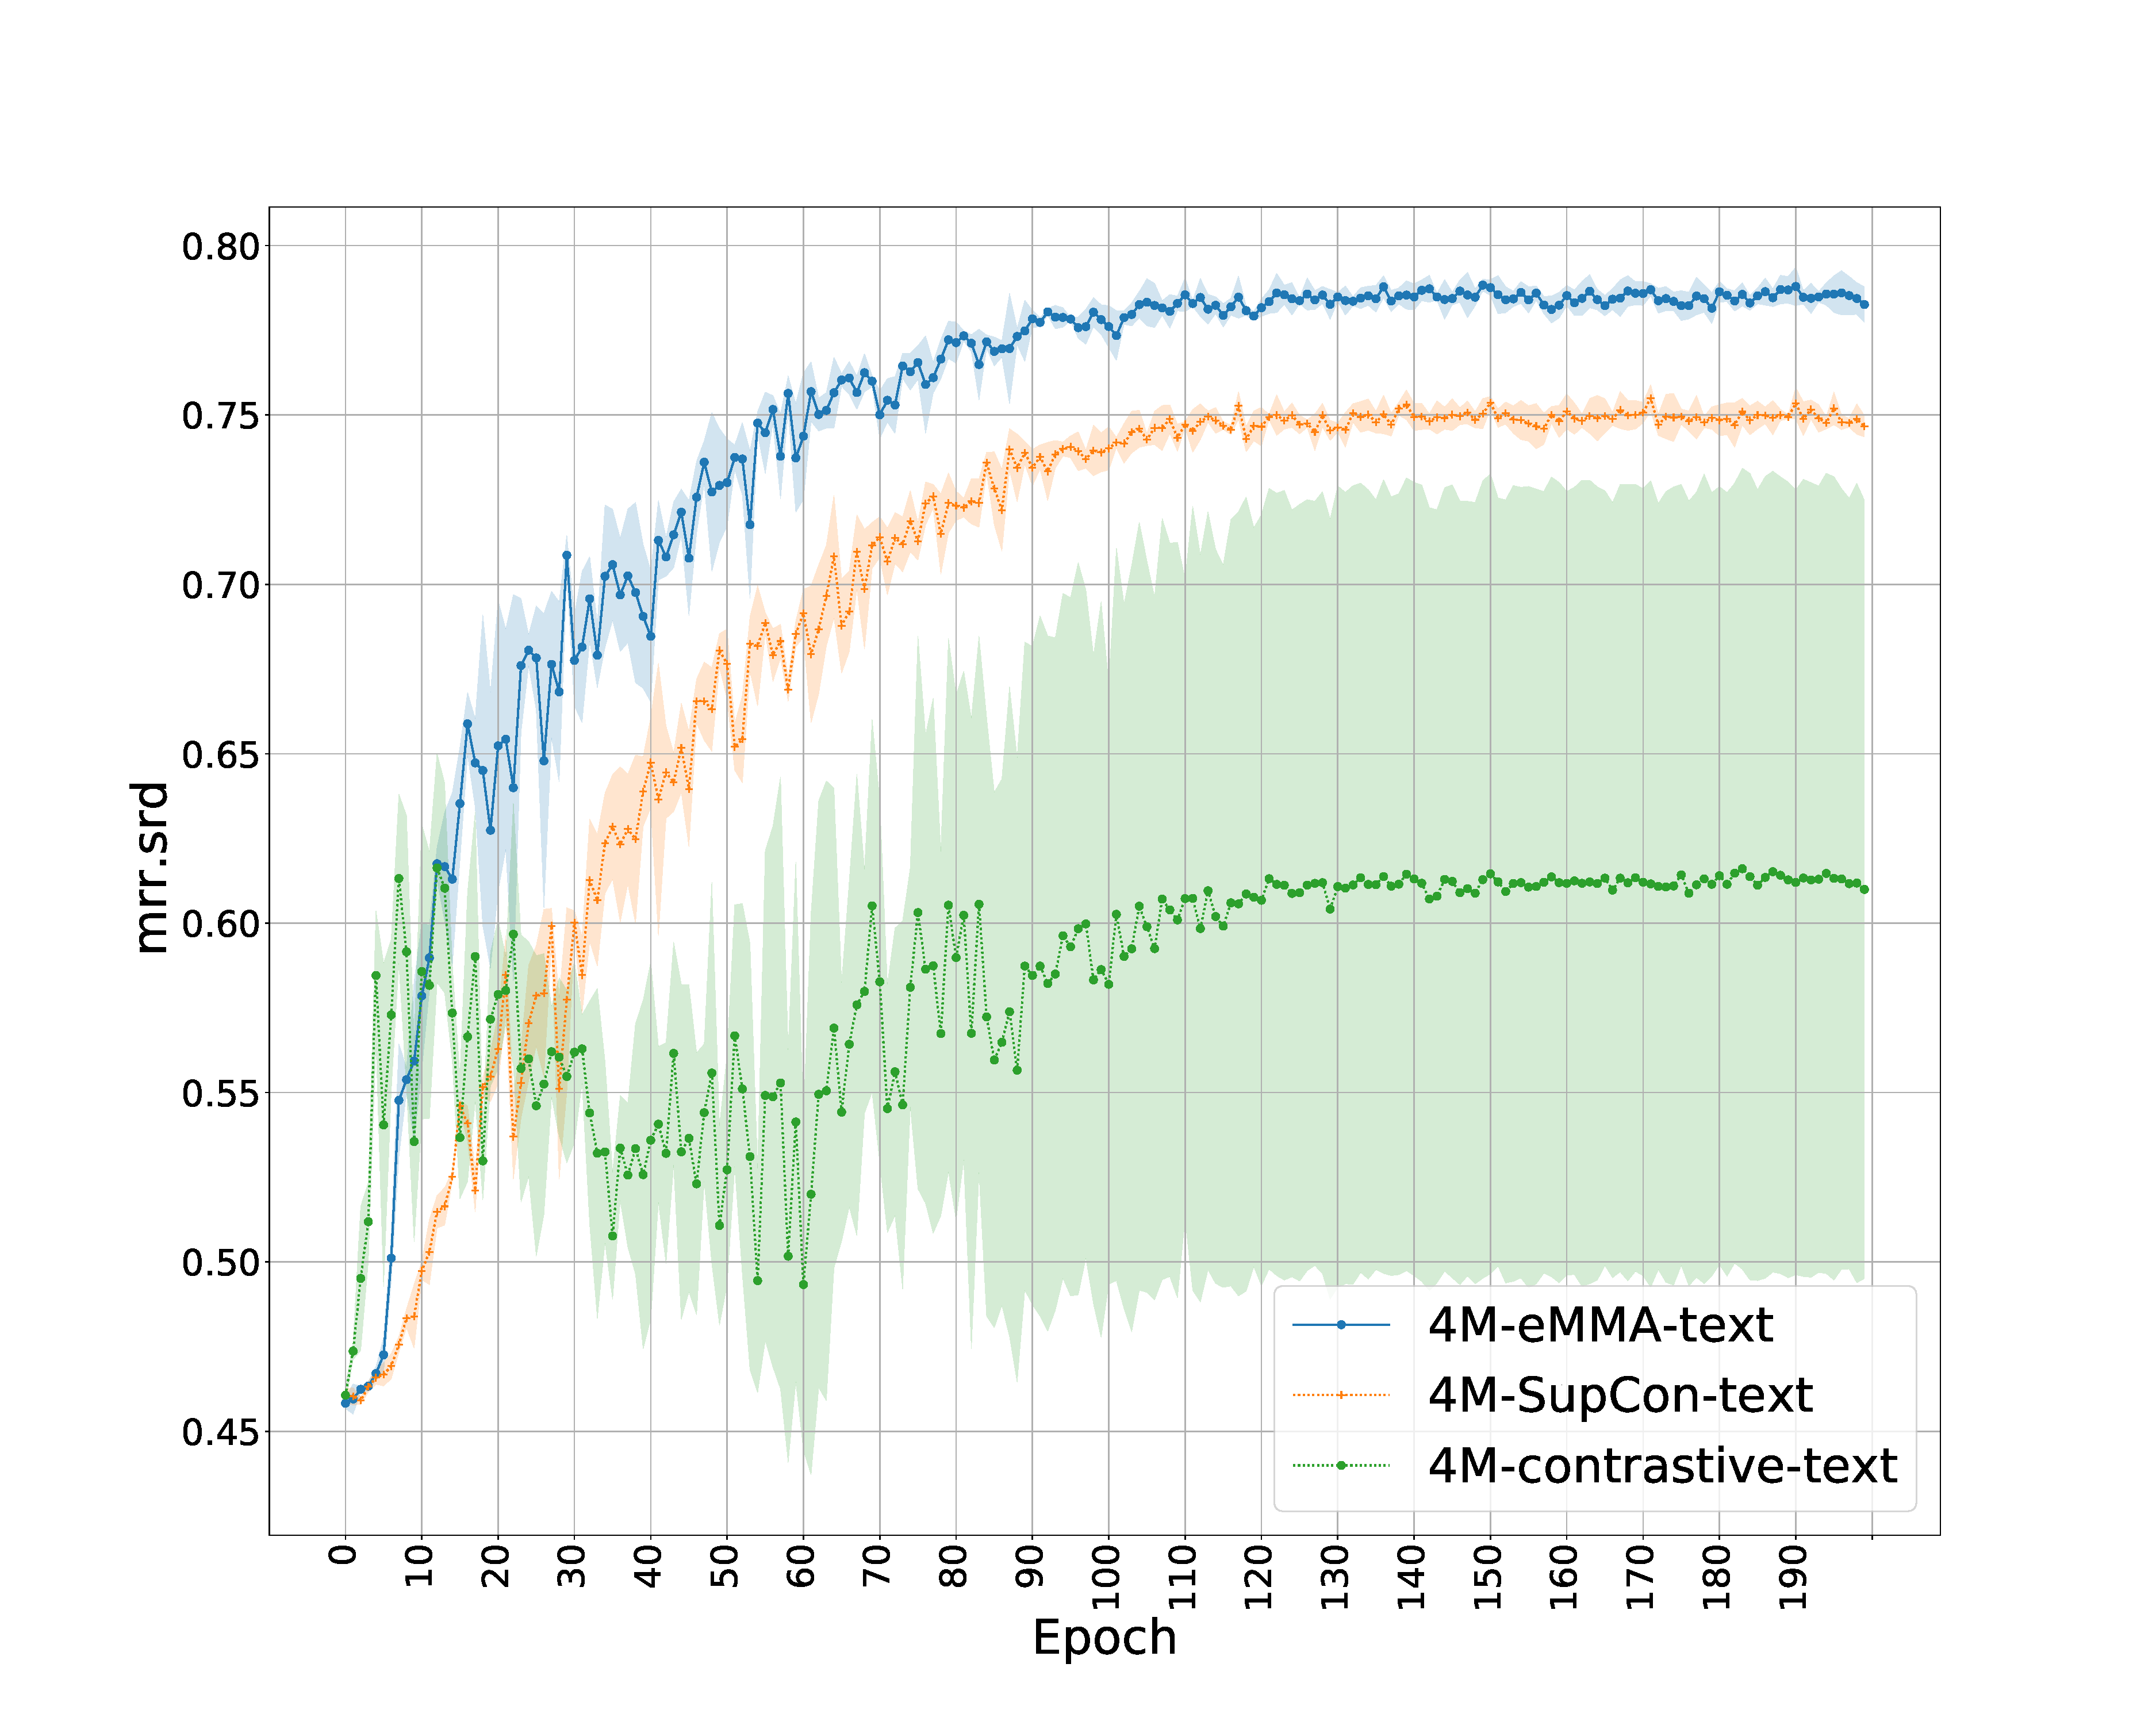
\includegraphics[width=.99\columnwidth]{Figures/average-seeds-epochs-mrr_ard.pdf}
\caption{Mean Reciprocal Rank (MRR) on the held-out test set when the text modality is ablated, averaged over 5 runs. Green is self-supervised contrastive learning, orange is supervised contrastive learning, and blue represents our proposed EMMA loss function. Higher is better.
}
\label{fig:epochs-mrr.srd}
\end{figure}

\begin{comment}
\begin{figure}[tbh]
\centering
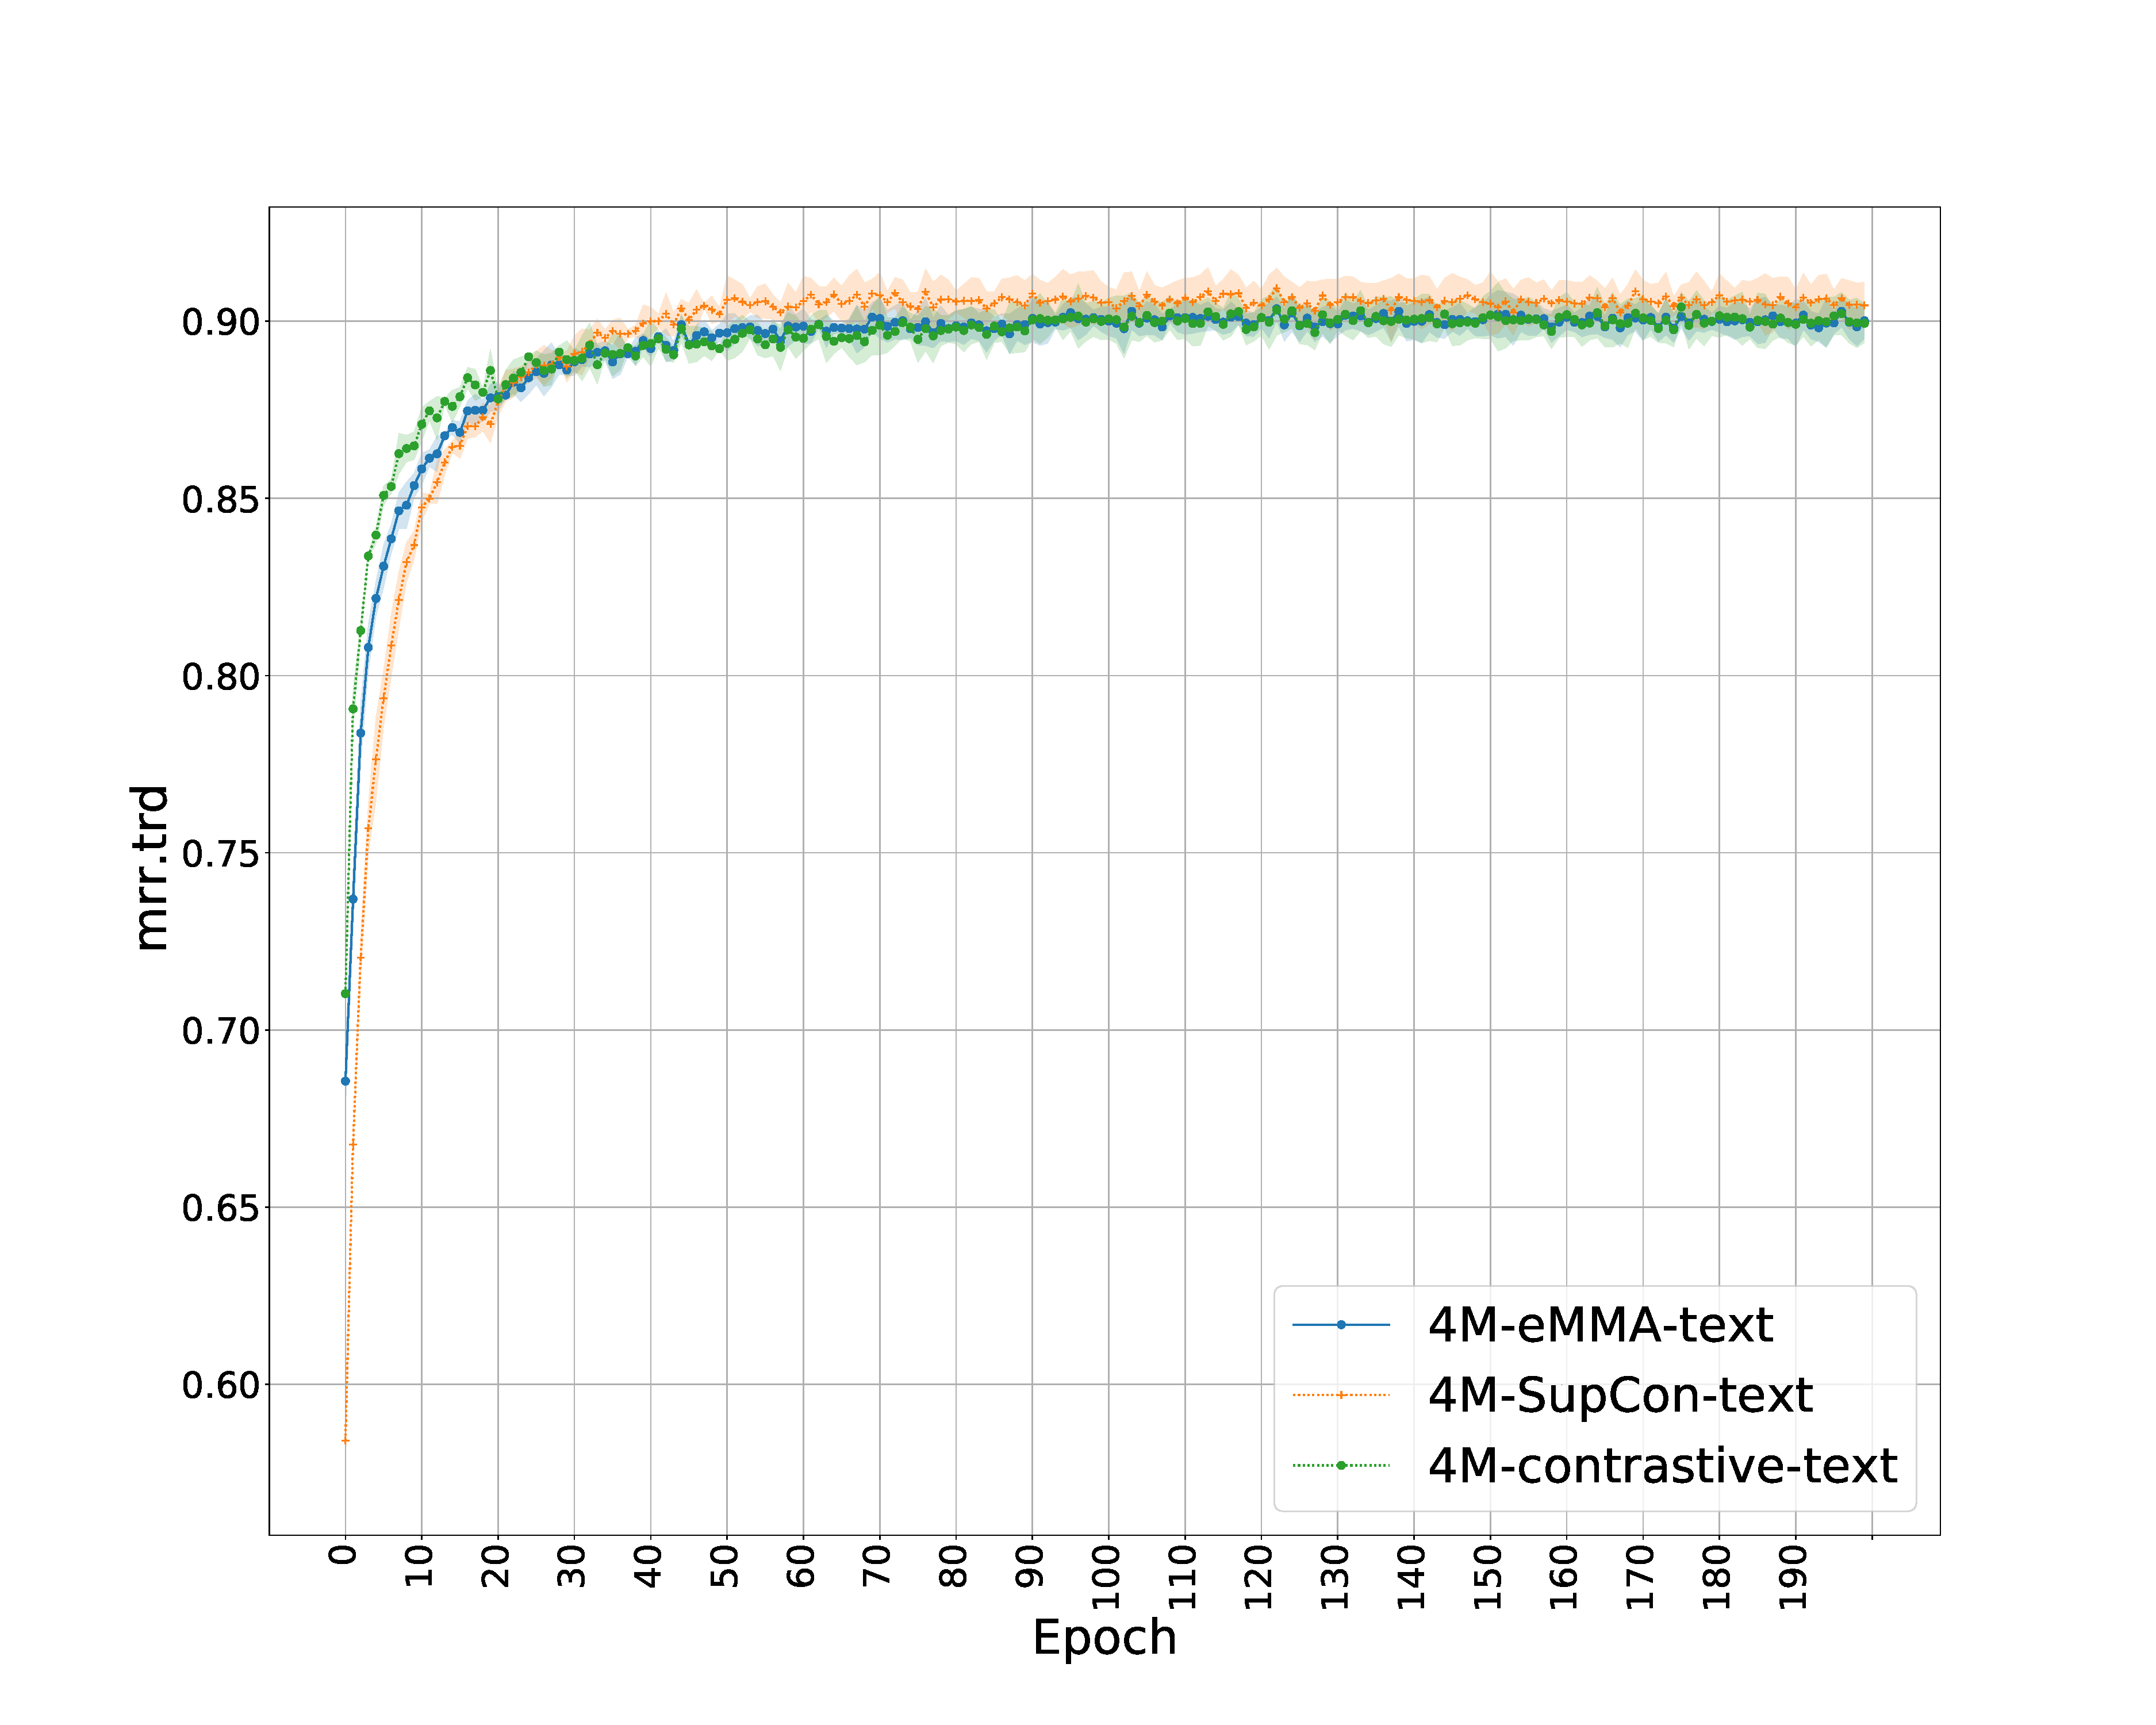
\includegraphics[width=.99\columnwidth]{Figures/average-seeds-epochs-mrr_lrd.pdf}
\caption{Mean Reciprocal Rank (MRR) on the held-out test set when the speech modality is ablated, averaged over 5 runs, for the downstream task of object retrieval when all objects are unique. Green is self-supervised contrastive learning, orange is supervised contrastive learning, and blue represents our proposed EMMA loss function. Higher is better. When speech as a modality is ablated, all tested methods perform similarly.
}
\label{fig:epochs-mrr.trd}
\end{figure}
\end{comment}

\begin{figure}[tbh]
\centering
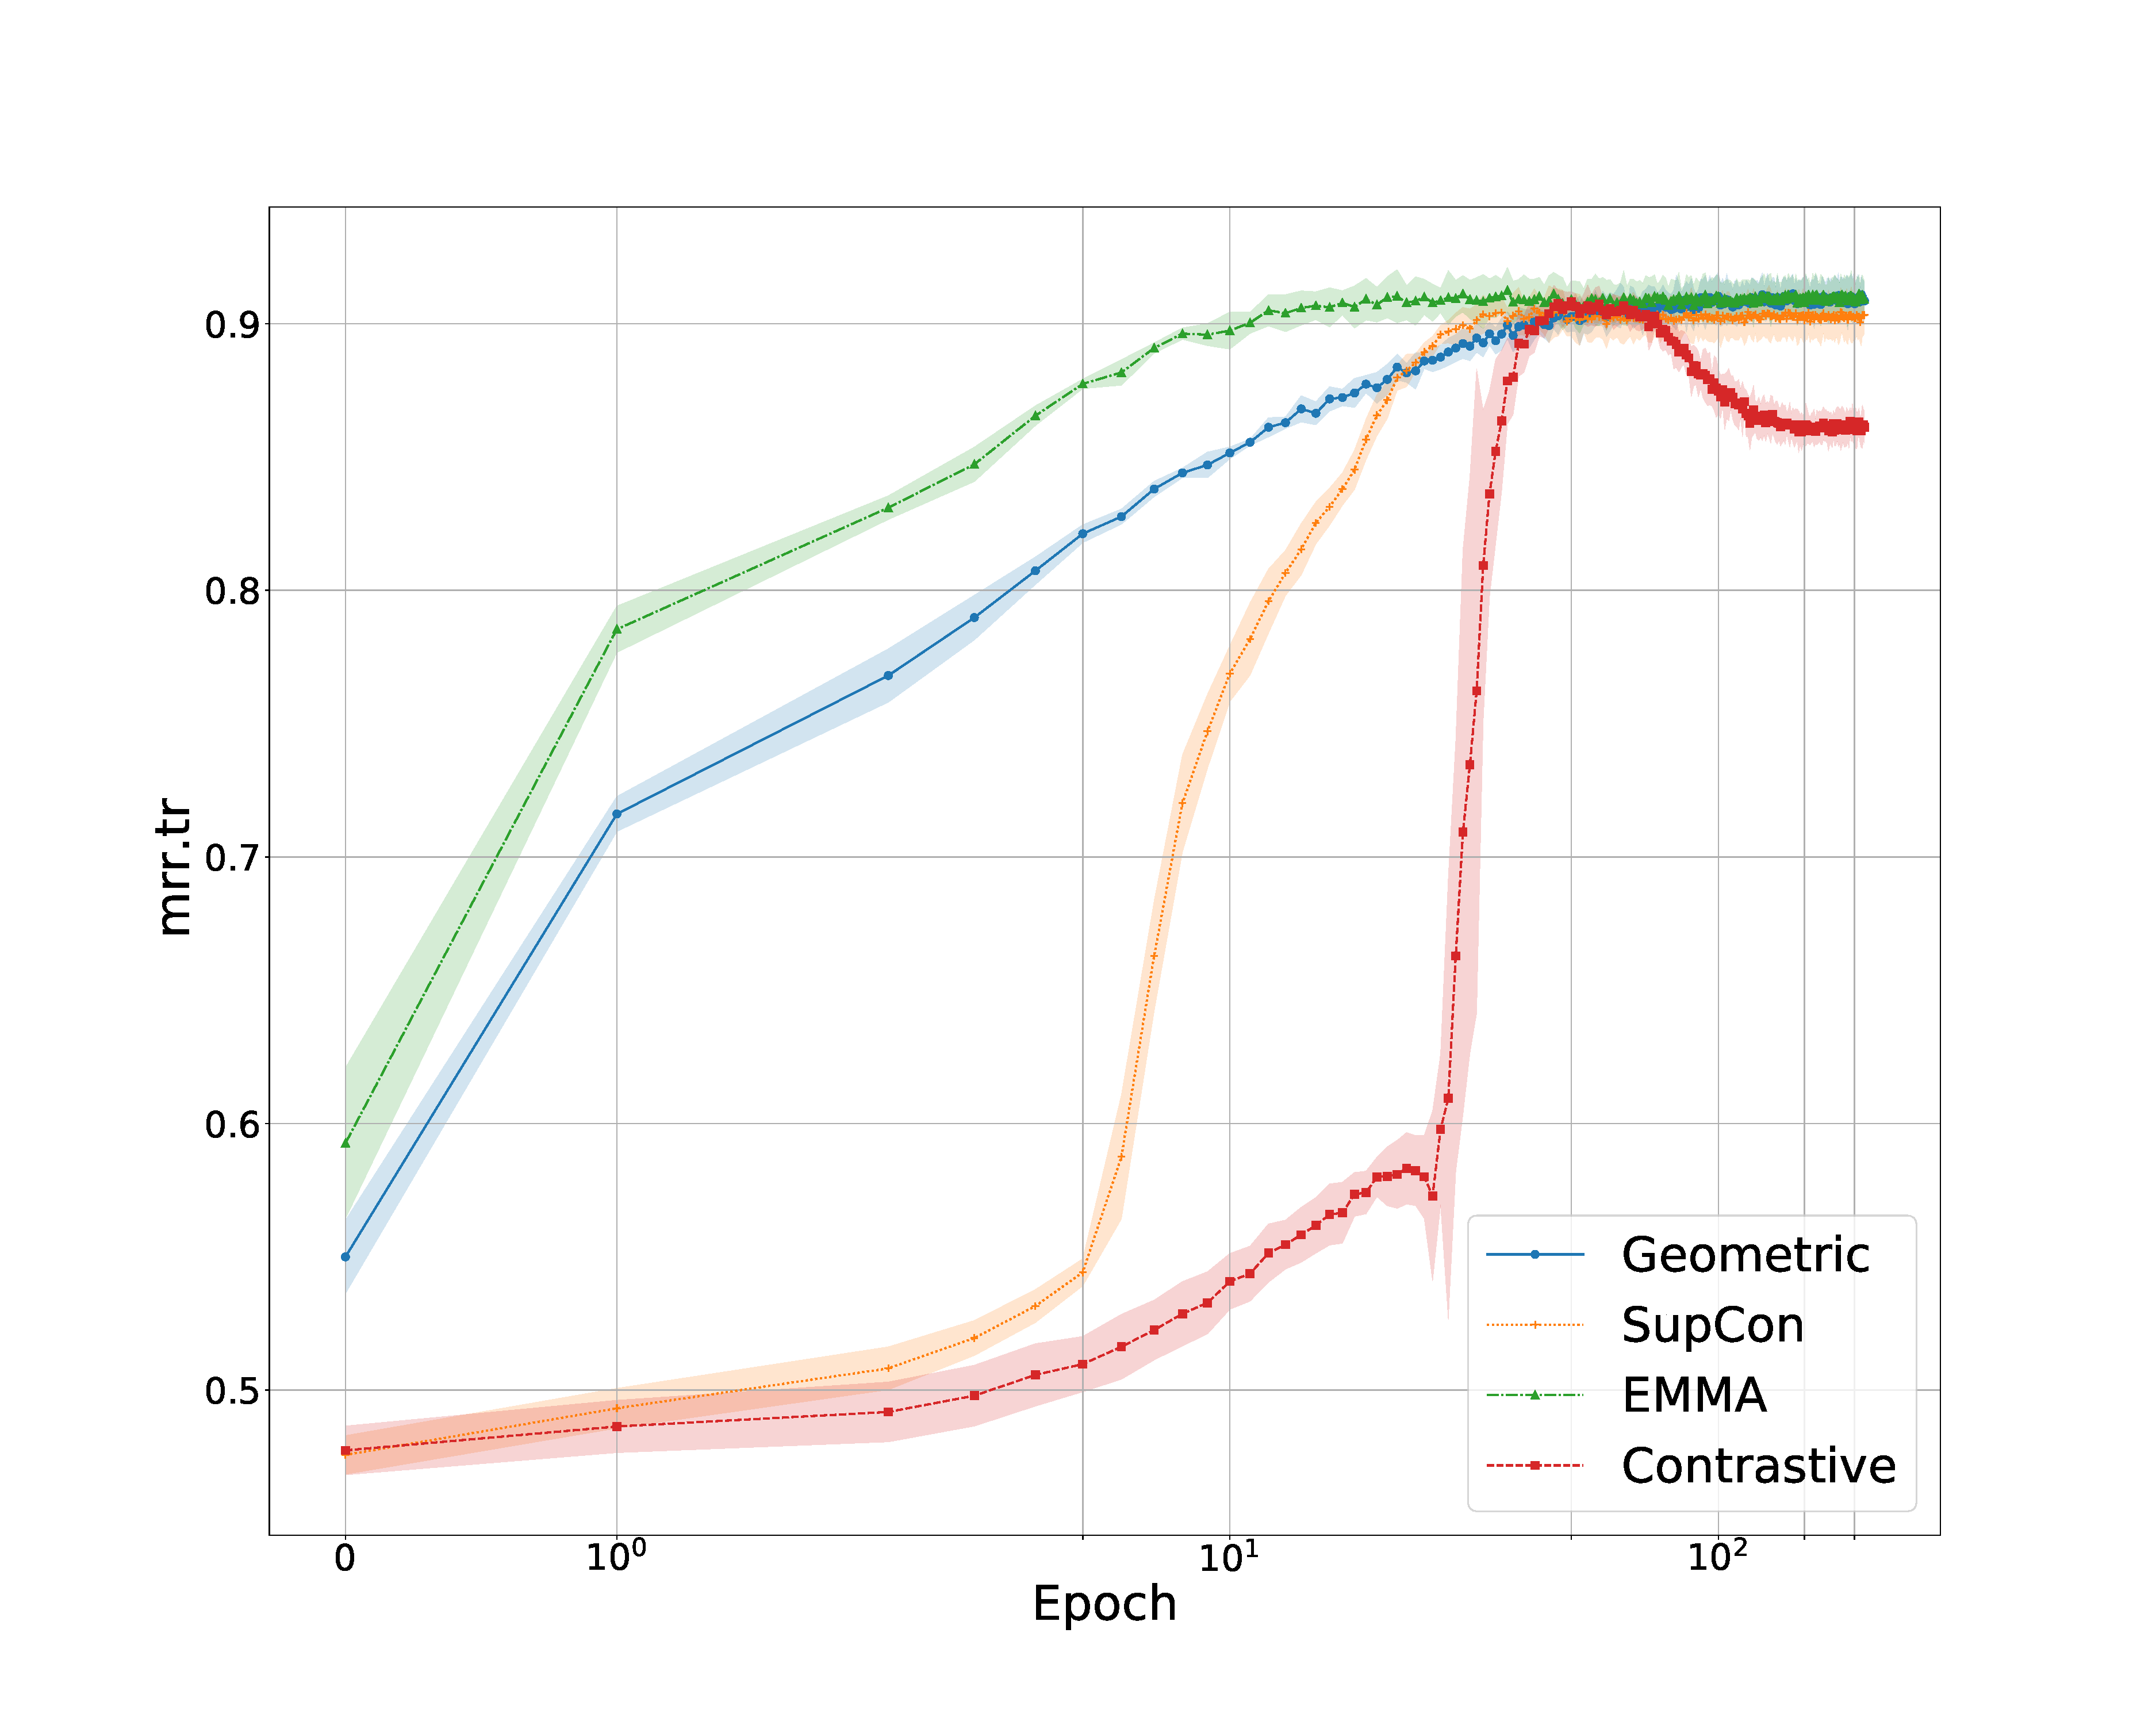
\includegraphics[width=.99\columnwidth]{Figures/average-seeds-epochs-mrr_lr.pdf}
\caption{Mean Reciprocal Rank (MRR) on the held-out test set when speech and depth modalities are ablated, averaged over 5 runs for the downstream task of object retrieval when all objects are unique.  Green is \ours{}, orange is \supcon{}, and blue represents our proposed \geom{} loss function. Higher is better.
}
% \todocmi{Maybe MRR is wrong and we should be looking at top-ranked result?}
\label{fig:epochs-mrr.lr}
\end{figure}



\begin{figure}[tbh]
\centering
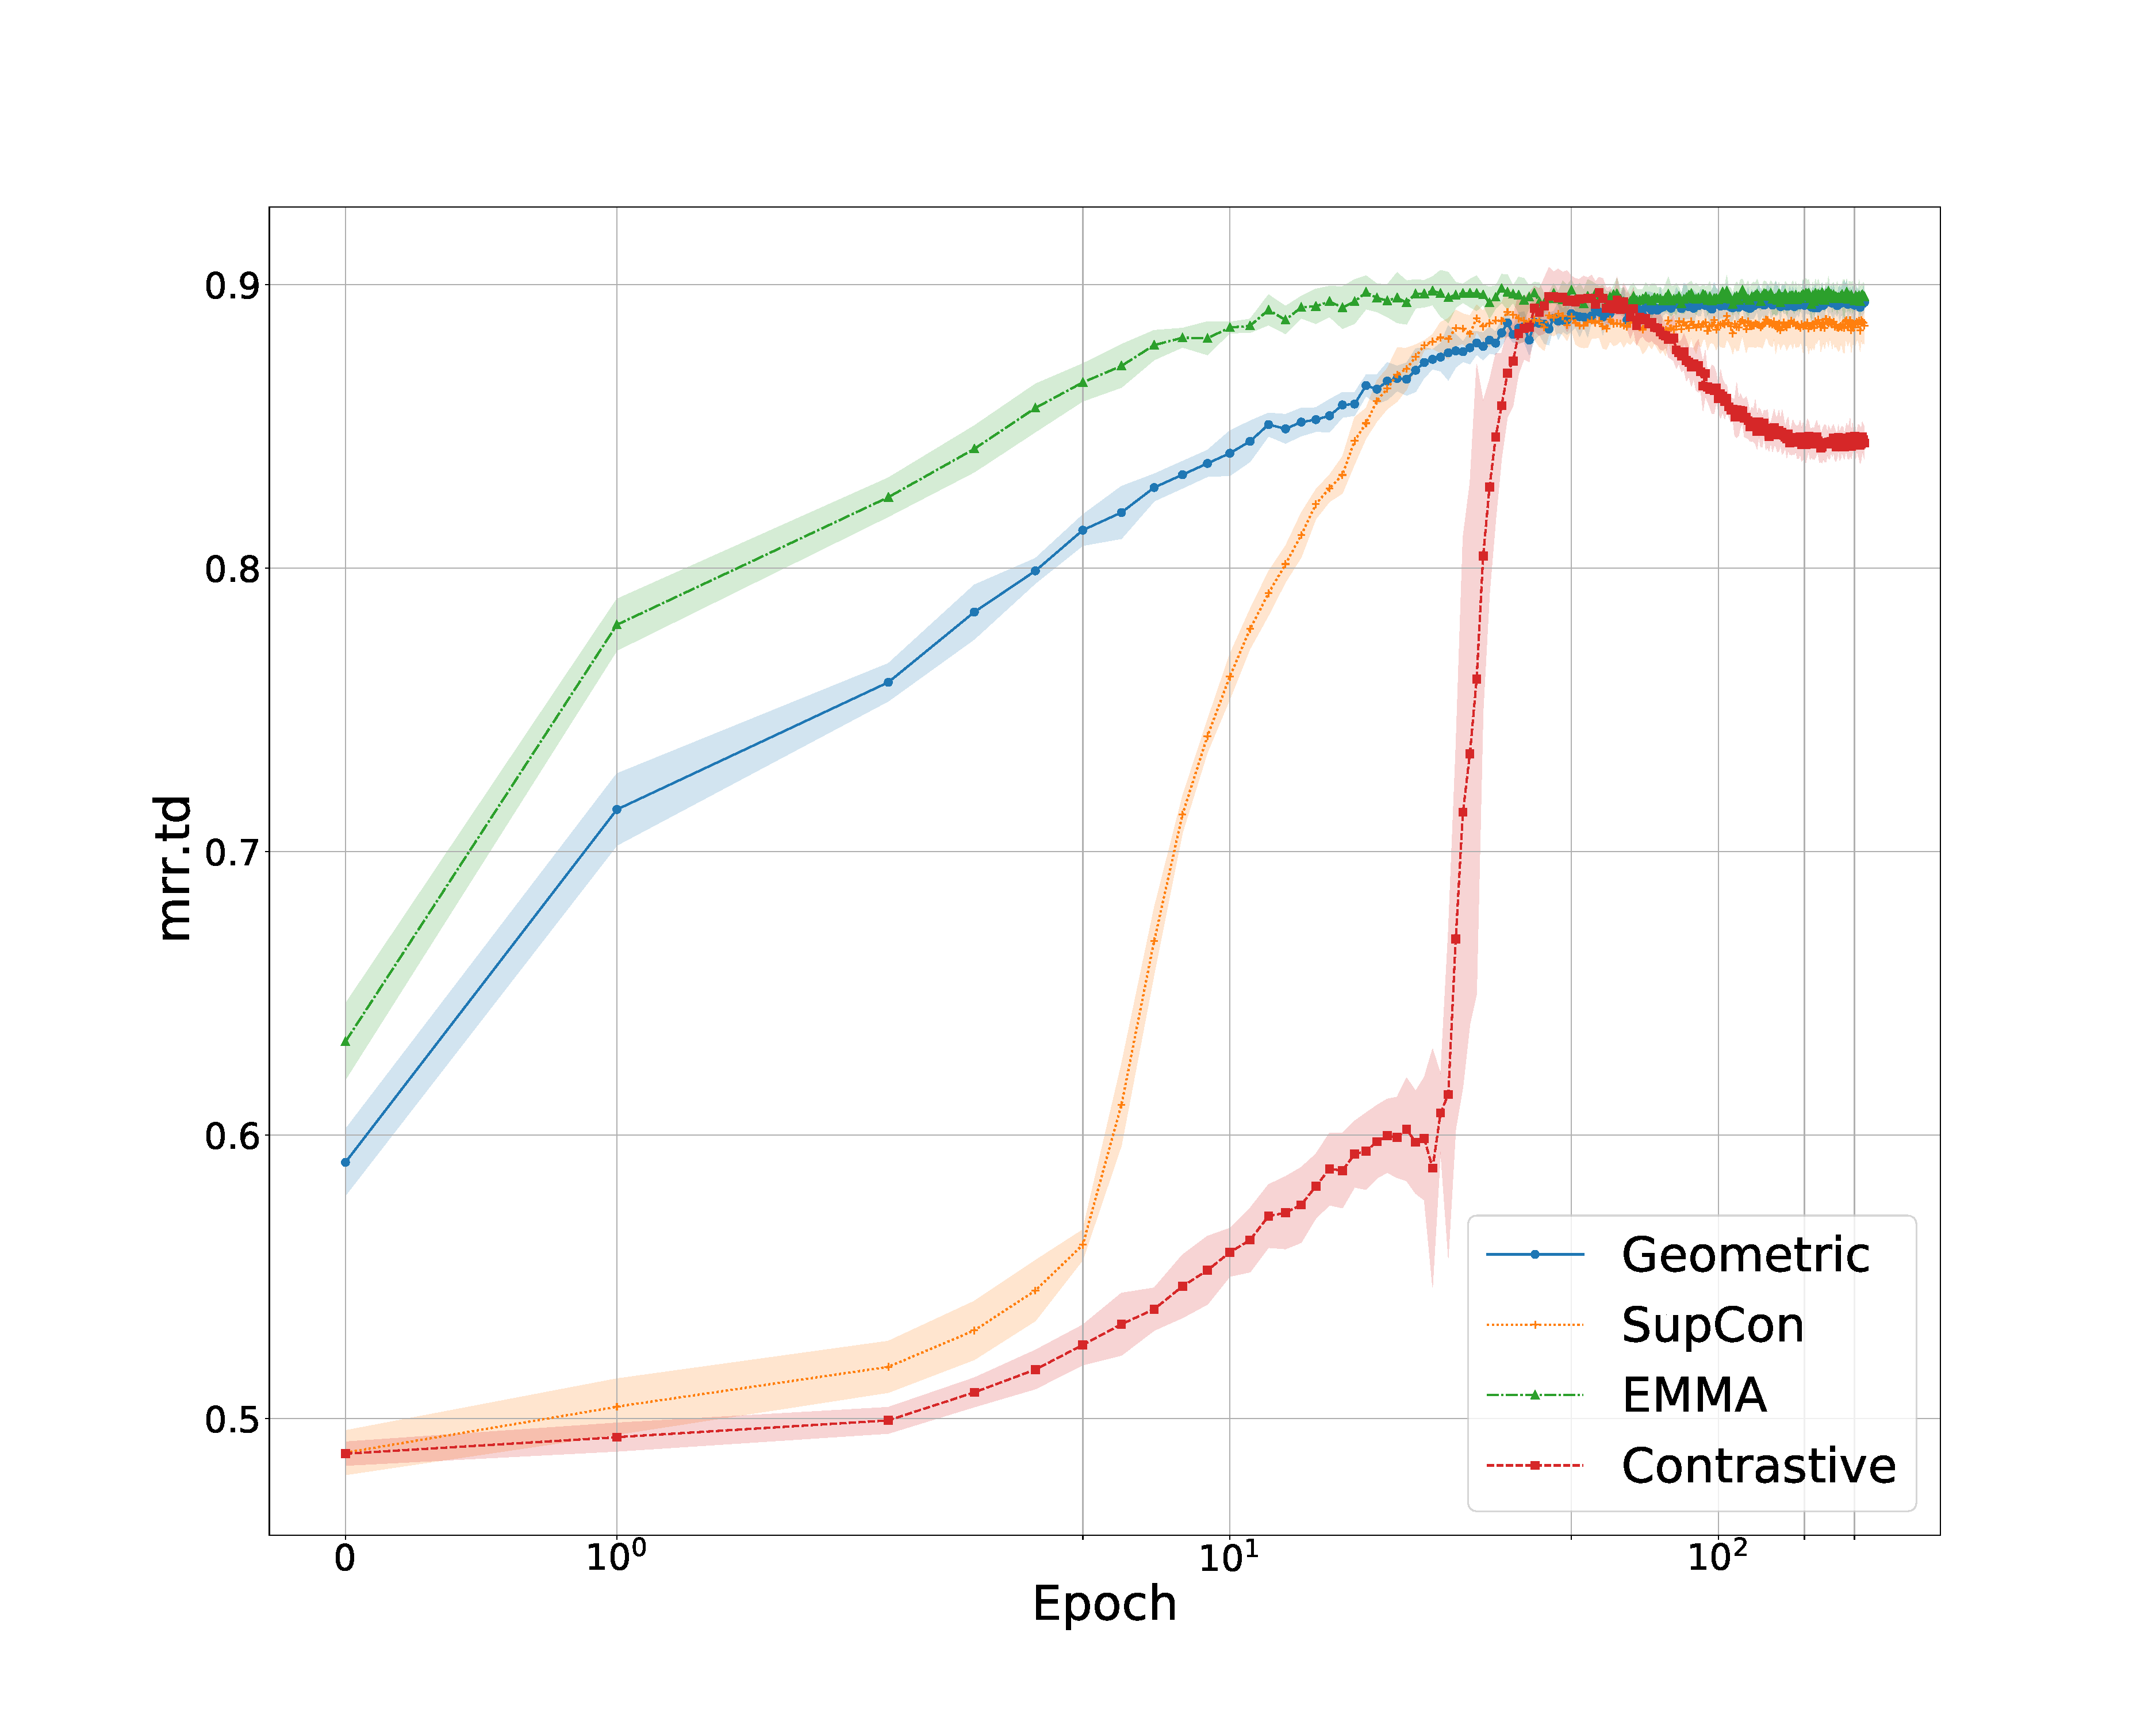
\includegraphics[width=.99\columnwidth]{Figures/average-seeds-epochs-mrr_ld.pdf}
\caption{Mean Reciprocal Rank (MRR) on the held-out test set when speech and RGB modalities are dropped averaged over 5 runs for the downstream task of object retrieval when all objects are unique. Green is \ours{}, orange is \supcon{}, and blue represents our proposed \geom{} loss function. Higher is better.
}
\label{fig:epochs-mrr.ld}
\end{figure}

\begin{figure*}[tbh]
\centering
% 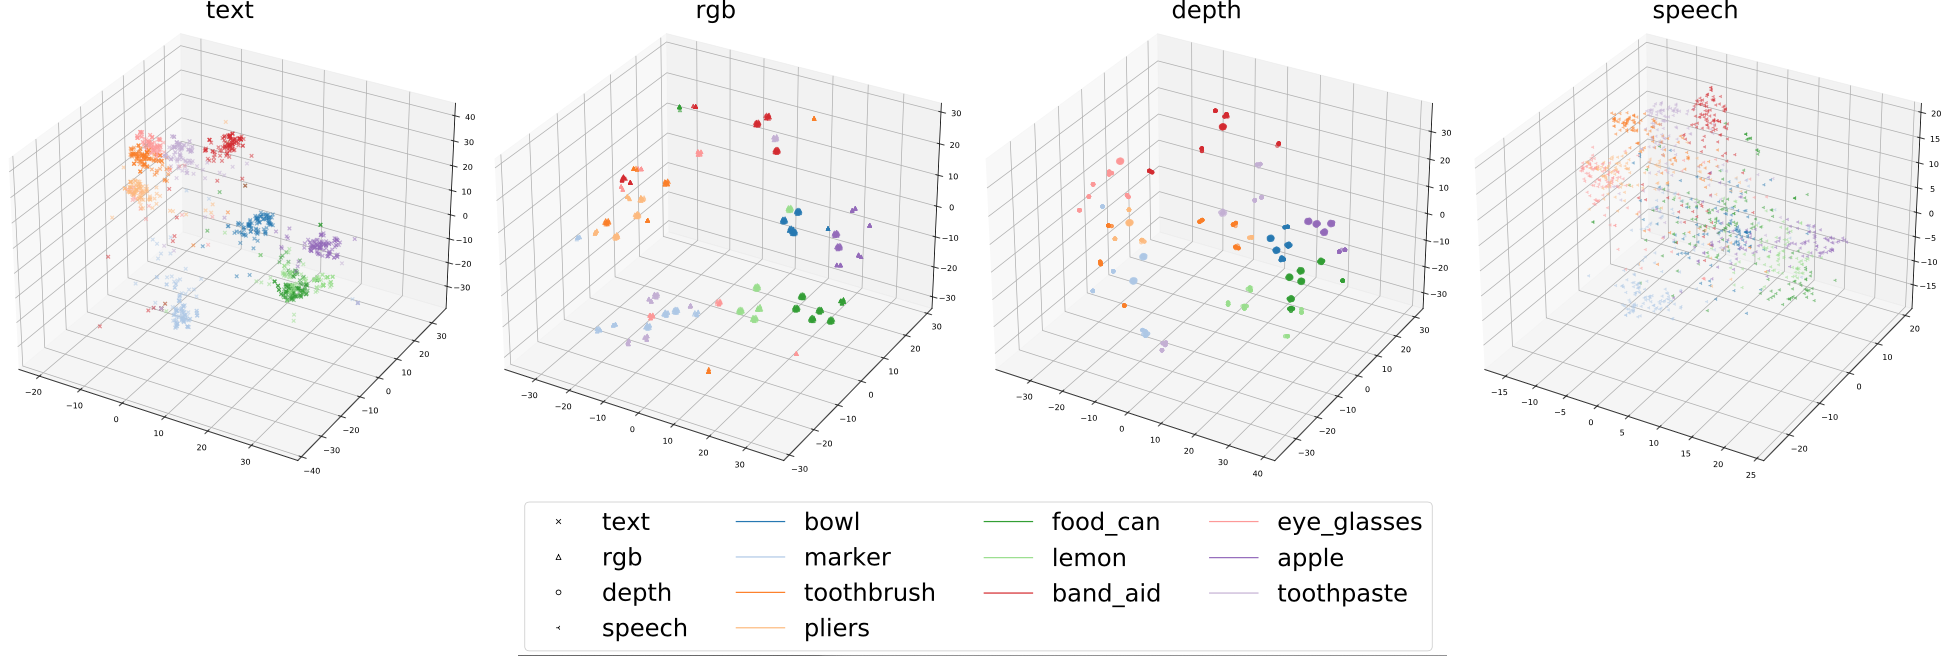
\includegraphics[width=1.99\columnwidth]{Figures/3D-tsne-4M-eMMA-cosine-submodalities-text-anchor-gold-no_neg_sampling-1024-sbs.png}
% 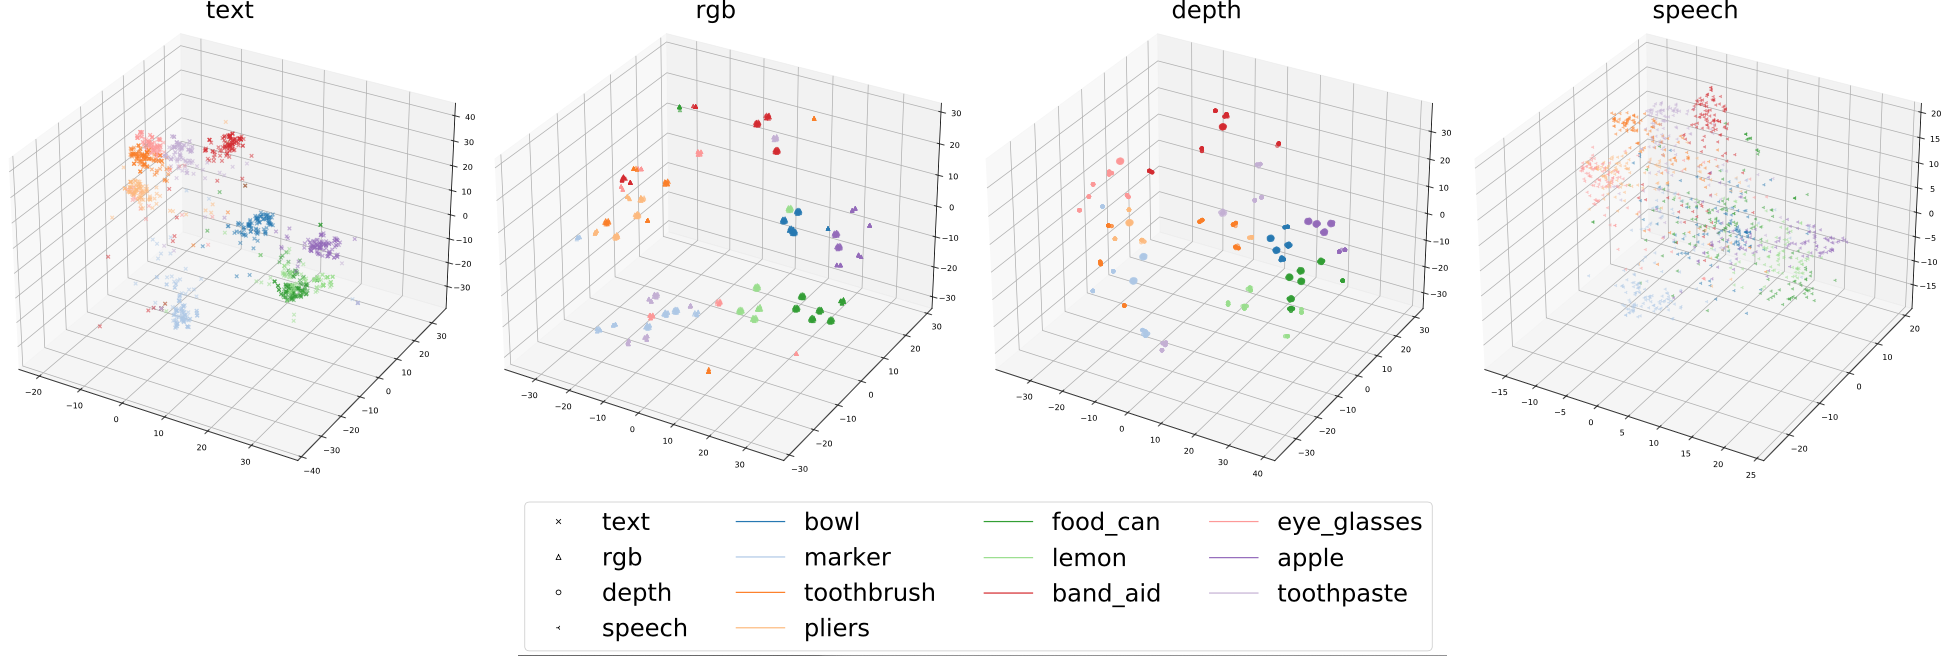
\includegraphics[width=1\columnwidth]{Figures/3D-tsne-4M-eMMA-cosine-submodalities-text-anchor-gold-no_neg_sampling-1024-sbs.png}
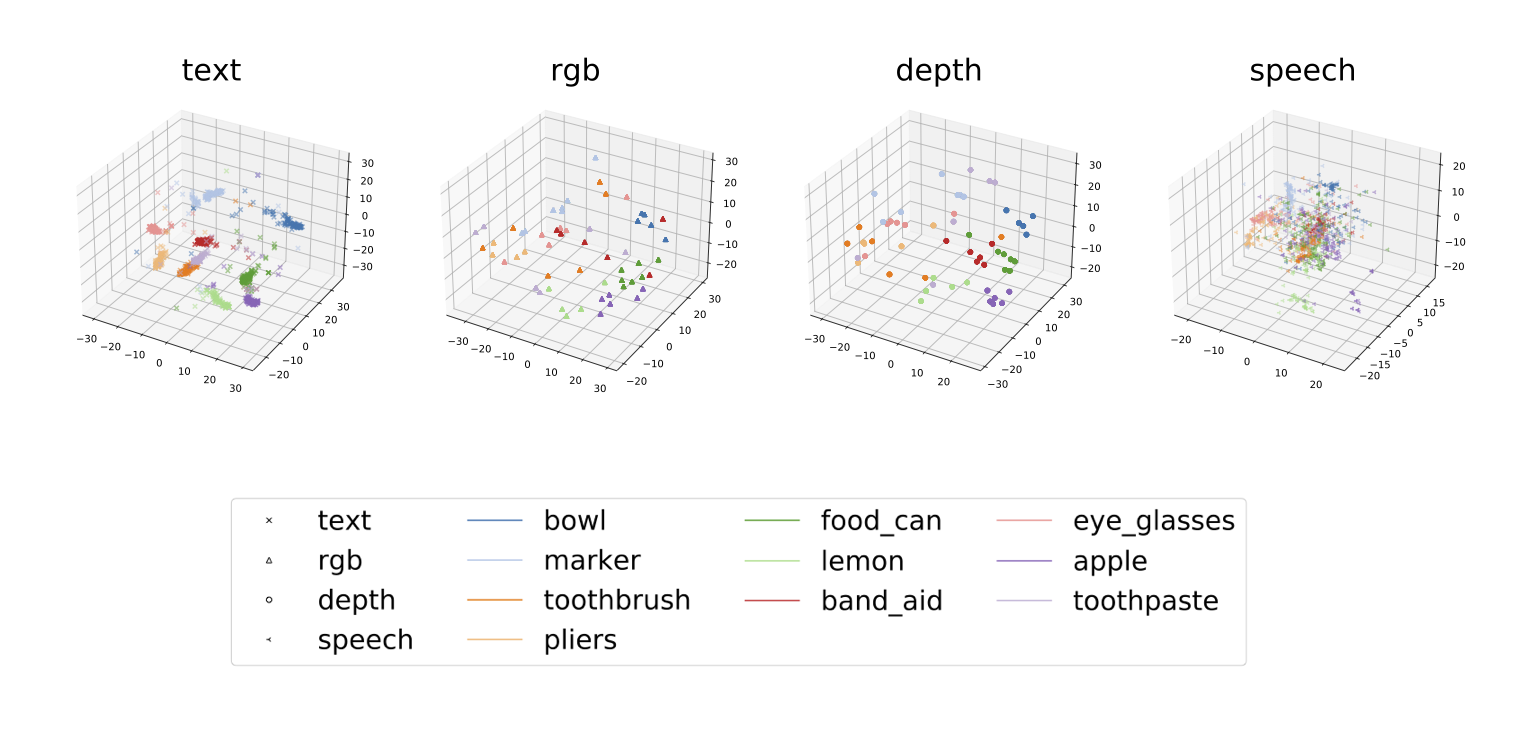
\includegraphics[width=1\columnwidth]{Figures/3D-tsne-exp-supcon-emma-lard-64-relu-SGD-0.001-unique_objects-gold-no_neg_sampling-1024-sbs.png}
\caption{3D T-SNE~\cite{van2008tsne} projection of test embeddings of 10 randomly selected classes of objects using our proposed \ours{}. Each modality is separately projected into a three-dimensional space. In a perfect embedding, all instances of a class would be clustered in identical areas of the embedding space across all modalities. We can see that \ours{} successfully encourages all four modalities to live in a common manifold, allowing accurate retrieval even when modalities are missing. 
}
\label{fig:3d-tsne}
\end{figure*}

% \subsection{Qualitative Results}
% \label{sec:Qualitative}
We look into the projection of the high-dimensional learned embeddings into a 
%2-dimensional and 
3-dimensional space using t-SNE~\cite{van2008tsne}, which is a dimensionality reduction technique to visualize high-dimensional data. T-SNE creates a probability distribution over pairs of high-dimensional data where similar pairs have a higher probability and dissimilar pairs have a lower probability. A similar probability distribution is also defined over pairs of data in the lower dimension (either 2D or 3D), and T-SNE minimizes the KL divergence between these two probability distributions.
% \textcolor{red}{\dots}\todo{explanation}. 
% \Cref{fig:2d-tsne} shows the projection of all test embeddings from all different modalities in a 2D space. As shown in the graph, instances of the same class but different modality are mapped to almost the same locations and are closer to each other.
\Cref{fig:3d-tsne} shows the projection onto 3D space to give a better view of the location of embeddings. Although these projections are not perfect, combined with the quantitative results, they demonstrate that our model is learning to map instances of the same class closer to each other regardless of their modalities.



% \begin{figure}[tbh]
% \centering
% 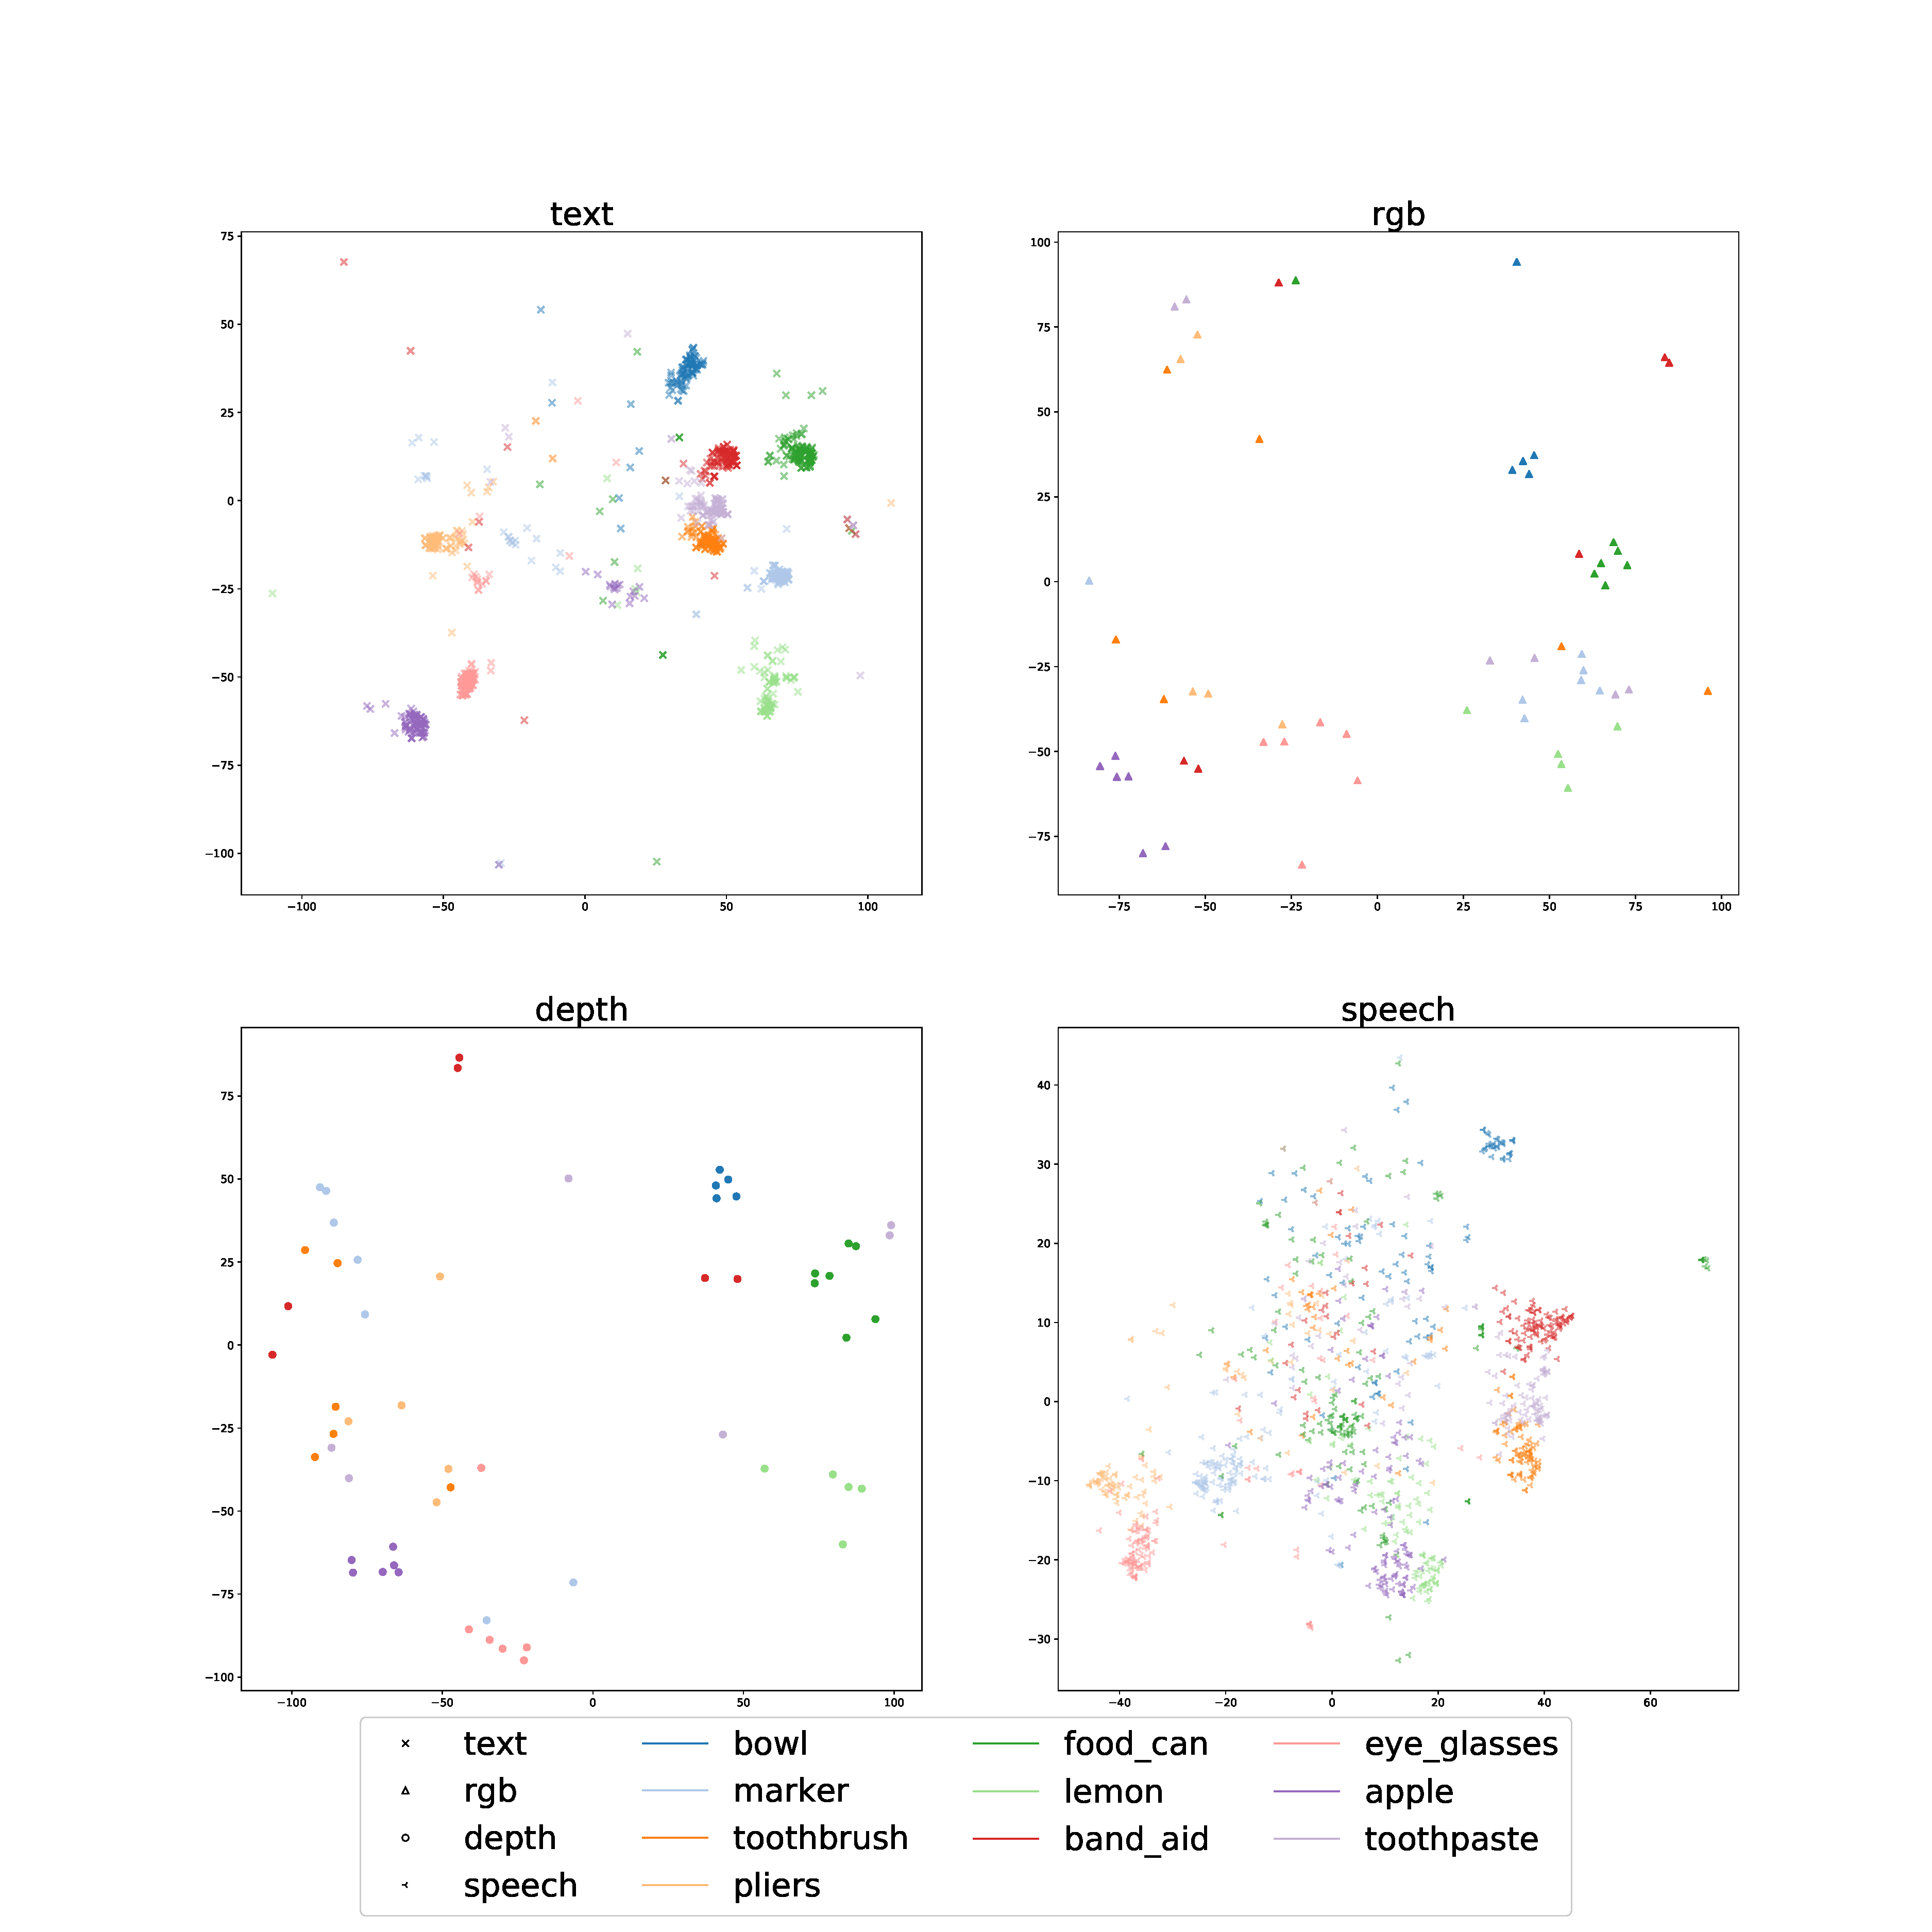
\includegraphics[width=.99\columnwidth]{Figures/2D-tsne-4M-eMMA-cosine-submodalities-text-anchor-gold-no_neg_sampling-1024.pdf}
% \caption{2D T-SNE~\cite{van2008tsne} projection of test embeddings of 10 randomly selected classes of objects using our proposed method. Each modality is separately projected into a two-dimensional space. \Rephrase{} \textcolor{red}{We may only want 3D}
% }
% \label{fig:2d-tsne}
% \end{figure}

% \todokdinline{Add the T-SNE projection for supervised contrastive loss as well.}

% \subsection{Failed Experiments}
% \todokdinline{I suppose I should remove this subsection, right?}
% We tried a lot of different approaches and they did not work better than our model or the baselines, but we list them here to save time for readers who want to try them.

% \subsubsection{Simple MMA}
% Copy text from \ref{sub:simple-mma} if we decide to keep this section.

% \subsubsection{Two Anchors}
% Since speech is similar to text in its usage when it comes to the downstream task of object retrieval (given a single language command, find the correct object among multiple objects), we decided to have text and speech as two anchors instead of having one anchor only. When there is one anchor, the distance between positive pairs text and speech is minimized and the distance between negative pairs are minimized. However, this is not related to the downstream task since we never want to find the correct speech for a given text or vice versa. The second term added to the last function is exactly similar to the loss function when speech is the anchor, and the first term is the same as when language is the anchor. Therefore, the performance is somewhere in the middle of those two approaches but more towards the speech when the metrics are computed based and speech matrices.

% \subsection{Example Prediction}



\subsection{Discussion}
Our proposed model performs well and learns fast, has been demonstrated to handle four modalities of shared information effectively, and is robust to test-time situations where information from one or more modalities is missing. 

However, there is still room for improvement. Specifically, the speech modality is harder to handle. \Cref{fig:3d-tsne} shows that although the relative position of instances are correct in the speech space, the distinction and clustering of different objects are not as good as the other three modalities.

Text seems to be the best clustered modality, and that makes sense because the variation in written text is much smaller than the other three modalities. Variation in speech is higher because of different accents, native language, gender, age, and etc., variation in RGB and depth is higher than text because of lightning conditions, object's texture and shape, the angle of camera, and other factors.

\begin{figure}[h!]
\centering
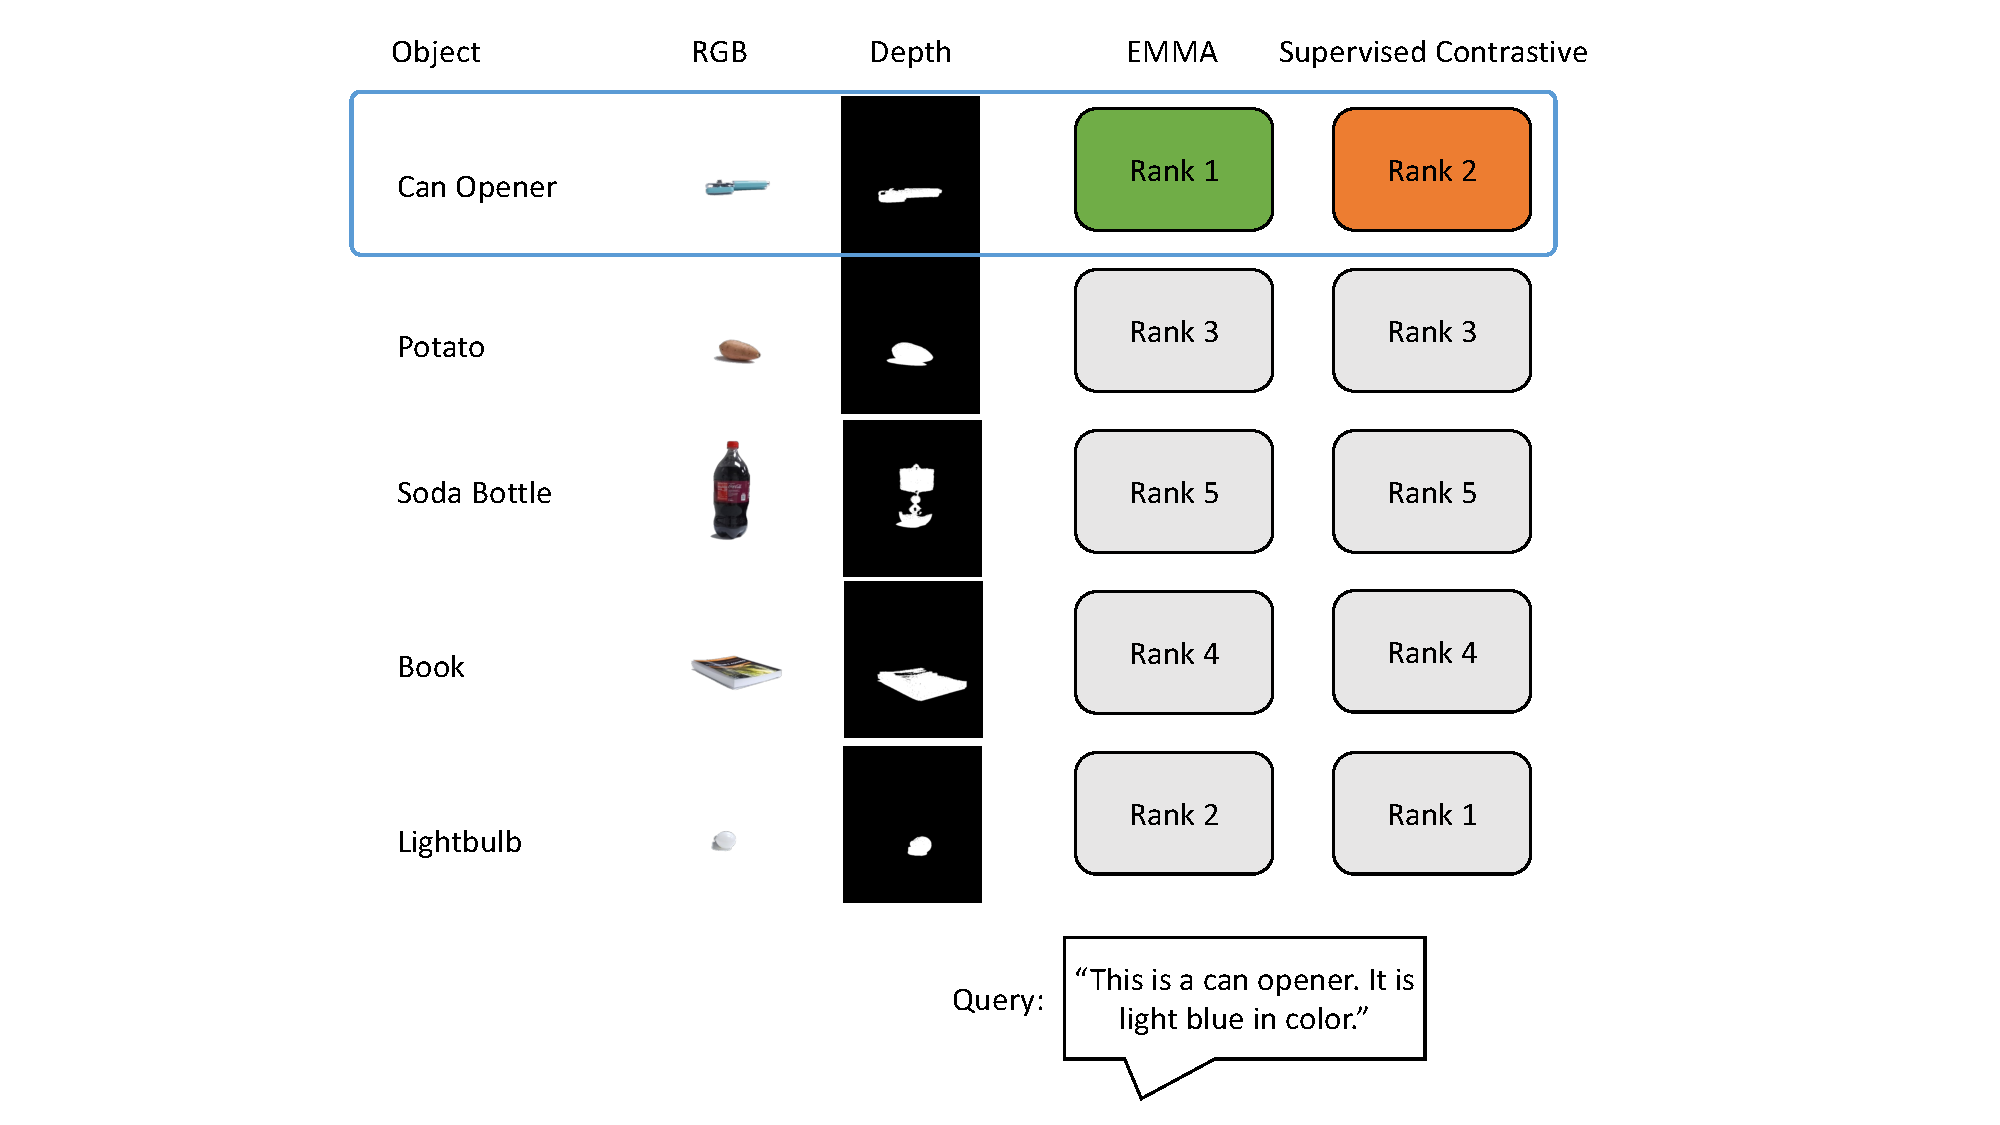
\includegraphics[width=1\columnwidth]{Figures/example-rankings.pdf}
\caption{\ours{} more accurately ranks objects and handles ambiguities with respect to a retrieval query compared to \supcon{}. Note that the phrase ``light blue'' in the query is very similar to ``light bulb'' and while \supcon{} confuses this and predicts light bulb as the correct object, \ours{} correctly identifies can opener as the intended object, and light bulb is ranked as the second object.
}
\label{fig:rankings}
\end{figure}

An example of the need to consider multiple modalities jointly is shown in \cref{fig:rankings}, showing how EMMA is able to correctly select an object instance from several similarly shaped and describable objects. 

%===================================================================

\section{Conclusion}
\label{sec:conclusion}


In this work, we have demonstrated the effectiveness of a novel approach to learning from high-dimensional multimodal information even when one or more modalities is unavailable at test time. Our approach performs well on an object retrieval task from a testbed that contains four separate modalities, consistent with information that might be available to a physical agent, and outperforms state of the art contrastive learning approaches. 
Our proposed method is general enough to be applied to a variety of multimodal retrieval problems, and is not limited to purely language-based image retrieval.
\todokdinline{Don't we need evidence for that?}

In future, this work will be extended to solve less clearly delineated problems; for example, differentiating among members of a class, as well as across classes. However, this work represents a significant step towards handling such retrieval problems, while not arbitrarily limiting the number of sensor and other modalities that can be incorporated. 

% Another future work is to improve the speech modality so it can contribute more to the training. Right now when text modality is dropped, the performance decreases by about 0.12. Ideally a better model should have the same performance in case of dropout when it is trained using all modalities.

%===================================================================


% ***************** The END of the paper *****************



\bibliography{tmlr}
\bibliographystyle{tmlr}

\appendix
\section{Appendix}
\label{sec:appendix}

\end{document}
